%%% Hlavní soubor. Zde se definují základní parametry a odkazuje se na ostatní části. %%%

%% Verze pro jednostranný tisk:
% Okraje: levý 40mm, pravý 25mm, horní a dolní 25mm
% (ale pozor, LaTeX si sám přidává 1in)
\documentclass[12pt,a4paper]{report}
\setlength\textwidth{145mm}
\setlength\textheight{247mm}
\setlength\oddsidemargin{15mm}
\setlength\evensidemargin{15mm}
\setlength\topmargin{0mm}
\setlength\headsep{0mm}
\setlength\headheight{0mm}
% \openright zařídí, aby následující text začínal na pravé straně knihy
\let\openright=\clearpage

%% Pokud tiskneme oboustranně:
% \documentclass[12pt,a4paper,twoside,openright]{report}
% \setlength\textwidth{145mm}
% \setlength\textheight{247mm}
% \setlength\oddsidemargin{14.2mm}
% \setlength\evensidemargin{0mm}
% \setlength\topmargin{0mm}
% \setlength\headsep{0mm}
% \setlength\headheight{0mm}
% \let\openright=\cleardoublepage

%% Vytváříme PDF/A-2u
\usepackage[a-2u]{pdfx}

%% Přepneme na českou sazbu a fonty Latin Modern
\usepackage[czech]{babel}
\usepackage{lmodern}
\usepackage[T1]{fontenc}
\usepackage{textcomp}

%% Použité kódování znaků: obvykle latin2, cp1250 nebo utf8:
\usepackage[utf8]{inputenc}

%%% Další užitečné balíčky (jsou součástí běžných distribucí LaTeXu)
\usepackage{amsmath}        % rozšíření pro sazbu matematiky
\usepackage{amsfonts}       % matematické fonty
\usepackage{amsthm}         % sazba vět, definic apod.
\usepackage{bbding}         % balíček s nejrůznějšími symboly
			    % (čtverečky, hvězdičky, tužtičky, nůžtičky, ...)
\usepackage{bm}             % tučné symboly (příkaz \bm)
\usepackage{graphicx}       % vkládání obrázků
\usepackage{rotating}
\usepackage[export]{adjustbox} % rámeček
\usepackage{fancyvrb}       % vylepšené prostředí pro strojové písmo
\usepackage{minted}         % balíček pro code highlight
\usepackage{indentfirst}    % zavede odsazení 1. odstavce kapitoly
\usepackage{natbib}         % zajištuje možnost odkazovat na literaturu
			    % stylem AUTOR (ROK), resp. AUTOR [ČÍSLO]
\usepackage[nottoc]{tocbibind} % zajistí přidání seznamu literatury,
                            % obrázků a tabulek do obsahu
\usepackage{icomma}         % inteligetní čárka v matematickém módu
\usepackage{dcolumn}        % lepší zarovnání sloupců v tabulkách
\usepackage{booktabs}       % lepší vodorovné linky v tabulkách
\usepackage{paralist}       % lepší enumerate a itemize
\usepackage{xcolor}         % barevná sazba

\usepackage{todonotes}

%%% Údaje o práci

% Název práce v jazyce práce (přesně podle zadání)
\def\NazevPrace{Vizualizace otevřených dat zveřejněných podle OFN pro úřední desky}

% Název práce v angličtině
\def\NazevPraceEN{Visualization of open data published according to the Formal Open Standard for public administration bulletin boards}

% Jméno autora
\def\AutorPrace{Evgenia Golubeva}

% Rok odevzdání
\def\RokOdevzdani{2022}

% Název katedry nebo ústavu, kde byla práce oficiálně zadána
% (dle Organizační struktury MFF UK, případně plný název pracoviště mimo MFF)
\def\Katedra{Katedra softwarového inženýrství}
\def\KatedraEN{Department of Software Engineering}

% Jedná se o katedru (department) nebo o ústav (institute)?
\def\TypPracoviste{Katedra}
\def\TypPracovisteEN{Department}

% Vedoucí práce: Jméno a příjmení s~tituly
\def\Vedouci{RNDr. Jakub Klímek, Ph.D.}

% Pracoviště vedoucího (opět dle Organizační struktury MFF)
\def\KatedraVedouciho{Katedra softwarového inženýrství}
\def\KatedraVedoucihoEN{Department of Software Engineering}

% Studijní program a obor
\def\StudijniProgram{Informatika}
\def\StudijniObor{Programování a vývoj software}

% Nepovinné poděkování (vedoucímu práce, konzultantovi, tomu, kdo
% zapůjčil software, literaturu apod.)
\def\Podekovani{%
\paragraph{Poděkování}

Chtěla bych poděkovat svému vedoucímu RNDr. Jakubovi Klímkovi, Ph.D. za pravidelné konzultace k práci a velmi přínosnou zpětnou vazbu při vývoji aplikace.
}

% Abstrakt (doporučený rozsah cca 80-200 slov; nejedná se o zadání práce)
\def\Abstrakt{
V rámci bakalářské práce byla navržena a vyvinuta aplikace, která vizualizuje informace z úředních desek, zveřejněné jako otevřená data podle nového jednotného a strojově čitelného formátu definovaného jako OFN (otevřená formální norma).
Aplikace je určena zájemcům ze široké veřejnosti, kterým umožňuje informace prohlížet a filtrovat, ale také poskytovatelům dat. Aplikace provádí validaci zveřejněných dat a přehledně zobrazuje případné nedostatky v datech.
K získávání dat využívá aplikace SPARQL endpointů Národního katalogu otevřených dat a Registru práv a povinností. Je navržena jako single-page application implementovaná v TypeScriptu s použitím frameworku React.
}

\def\AbstraktEN{%
The Bachelor thesis is about the design and implementation of a web application which visualizes data from public administration bulletin boards. It uses open data published according to a new machine-readable format specified as a Formal Open Standard.
The application is intended not only for users from the general public who can use it to search and filter information from bulletin boards but also for data publishers. The application performs validation of published data and clearly displays any deficiencies.
To retrieve data the application uses the SPARQL endpoint of the National Data Catalog. It is implemented as a single-page application in TypeScript using React framework.

}

% 3 až 5 klíčových slov (doporučeno), každé uzavřeno ve složených závorkách
\def\KlicovaSlova{%
{otevřená data} {otevřená formální norma} {úřední desky} {webová aplikace} {vizualizace}
}
\def\KlicovaSlovaEN{%
{open data} {bulletin boards} {web aplication} {visualization} 
}

%% Balíček hyperref, kterým jdou vyrábět klikací odkazy v PDF,
%% ale hlavně ho používáme k uložení metadat do PDF (včetně obsahu).
%% Většinu nastavítek přednastaví balíček pdfx.
\hypersetup{unicode}
\hypersetup{breaklinks=true}

%% Definice různých užitečných maker (viz popis uvnitř souboru)
%%% Tento soubor obsahuje definice různých užitečných maker a prostředí %%%
%%% Další makra připisujte sem, ať nepřekáží v ostatních souborech.     %%%

%%% Drobné úpravy stylu

% Tato makra přesvědčují mírně ošklivým trikem LaTeX, aby hlavičky kapitol
% sázel příčetněji a nevynechával nad nimi spoustu místa. Směle ignorujte.
\makeatletter
\def\@makechapterhead#1{
  {\parindent \z@ \raggedright \normalfont
   \Huge\bfseries \thechapter. #1
   \par\nobreak
   \vskip 20\p@
}}
\def\@makeschapterhead#1{
  {\parindent \z@ \raggedright \normalfont
   \Huge\bfseries #1
   \par\nobreak
   \vskip 20\p@
}}
\makeatother

% Toto makro definuje kapitolu, která není očíslovaná, ale je uvedena v obsahu.
\def\chapwithtoc#1{
\chapter*{#1}
\addcontentsline{toc}{chapter}{#1}
}

% Trochu volnější nastavení dělení slov, než je default.
\lefthyphenmin=2
\righthyphenmin=2

% Zapne černé "slimáky" na koncích řádků, které přetekly, abychom si
% jich lépe všimli.
% \overfullrule=1mm

%%% Makra pro definice, věty, tvrzení, příklady, ... (vyžaduje baliček amsthm)

\theoremstyle{plain}
\newtheorem{veta}{Věta}
\newtheorem{lemma}[veta]{Lemma}
\newtheorem{tvrz}[veta]{Tvrzení}

\theoremstyle{plain}
\newtheorem{definice}{Definice}

\theoremstyle{remark}
\newtheorem*{dusl}{Důsledek}
\newtheorem*{pozn}{Poznámka}
\newtheorem*{prikl}{Příklad}

%%% Prostředí pro důkazy

\newenvironment{dukaz}{
  \par\medskip\noindent
  \textit{Důkaz}.
}{
\newline
\rightline{$\qedsymbol$}
}

%%% Prostředí pro sazbu kódu, případně vstupu/výstupu počítačových
%%% programů. (Vyžaduje balíček fancyvrb -- fancy verbatim.)

\DefineVerbatimEnvironment{code}{Verbatim}{fontsize=\small, frame=single}

%%% Prostor reálných, resp. přirozených čísel
\newcommand{\R}{\mathbb{R}}
\newcommand{\N}{\mathbb{N}}

%%% Užitečné operátory pro statistiku a pravděpodobnost
\DeclareMathOperator{\pr}{\textsf{P}}
\DeclareMathOperator{\E}{\textsf{E}\,}
\DeclareMathOperator{\var}{\textrm{var}}
\DeclareMathOperator{\sd}{\textrm{sd}}

%%% Příkaz pro transpozici vektoru/matice
\newcommand{\T}[1]{#1^\top}

%%% Vychytávky pro matematiku
\newcommand{\goto}{\rightarrow}
\newcommand{\gotop}{\stackrel{P}{\longrightarrow}}
\newcommand{\maon}[1]{o(n^{#1})}
\newcommand{\abs}[1]{\left|{#1}\right|}
\newcommand{\dint}{\int_0^\tau\!\!\int_0^\tau}
\newcommand{\isqr}[1]{\frac{1}{\sqrt{#1}}}

%%% Vychytávky pro tabulky
\newcommand{\pulrad}[1]{\raisebox{1.5ex}[0pt]{#1}}
\newcommand{\mc}[1]{\multicolumn{1}{c}{#1}}

%%% popisek u příkazu autoref
\def\chapterautorefname{kapitola}
\def\sectionautorefname{sekce}
\def\subsectionautorefname{část}
\def\figureautorefname{obrázek}


%% Titulní strana a různé povinné informační strany
\begin{document}
%%% Titulní strana práce a další povinné informační strany

%%% Titulní strana práce

\pagestyle{empty}
\hypersetup{pageanchor=false}

\begin{center}

\centerline{\mbox{
\includegraphics[width=166mm]{../img/logo-cs.pdf}}}

\vspace{-8mm}
\vfill

{\bf\Large BAKALÁŘSKÁ PRÁCE}

\vfill

{\LARGE\AutorPrace}

\vspace{15mm}

{\LARGE\bfseries\NazevPrace}

\vfill

\Katedra

\vfill

{
\centerline{\vbox{\halign{\hbox to 0.45\hsize{\hfil #}&\hskip 0.5em\parbox[t]{0.45\hsize}{\raggedright #}\cr
Vedoucí bakalářské práce:&\Vedouci \cr
\noalign{\vspace{2mm}}
Studijní program:&\StudijniProgram \cr
\noalign{\vspace{2mm}}
Studijní obor:&\StudijniObor \cr
}}}}

\vfill

% Zde doplňte rok
Praha \RokOdevzdani

\end{center}

\newpage

%%% Následuje vevázaný list -- kopie podepsaného "Zadání bakalářské práce".
%%% Toto zadání NENÍ součástí elektronické verze práce, nescanovat.

%%% Strana s čestným prohlášením k bakalářské práci

\openright
\hypersetup{pageanchor=true}
\pagestyle{plain}
\pagenumbering{roman}
\vglue 0pt plus 1fill

\noindent
Prohlašuji, že jsem tuto bakalářskou práci vypracoval(a) samostatně a výhradně
s~použitím citovaných pramenů, literatury a dalších odborných zdrojů.
Tato práce nebyla využita k získání jiného nebo stejného titulu.

\medskip\noindent
Beru na~vědomí, že se na moji práci vztahují práva a povinnosti vyplývající
ze zákona č. 121/2000 Sb., autorského zákona v~platném znění, zejména skutečnost,
že Univerzita Karlova má právo na~uzavření licenční smlouvy o~užití této
práce jako školního díla podle §60 odst. 1 autorského zákona.

\vspace{10mm}

\hbox{\hbox to 0.5\hsize{%
V \hbox to 6em{\dotfill} dne \hbox to 6em{\dotfill}
\hss}\hbox to 0.5\hsize{\dotfill\quad}}
\smallskip
\hbox{\hbox to 0.5\hsize{}\hbox to 0.5\hsize{\hfil Podpis autora\hfil}}

\vspace{20mm}
\newpage

%%% Poděkování

\openright

\noindent
\Podekovani

\newpage

%%% Povinná informační strana bakalářské práce

\openright

\vbox to 0.5\vsize{
\setlength\parindent{0mm}
\setlength\parskip{5mm}

Název práce:
\NazevPrace

Autor:
\AutorPrace

\TypPracoviste:
\Katedra

Vedoucí bakalářské práce:
\Vedouci, \KatedraVedouciho

Abstrakt:
\Abstrakt

Klíčová slova:
\KlicovaSlova


\vss}\nobreak\vbox to 0.49\vsize{
\setlength\parindent{0mm}
\setlength\parskip{5mm}

Title:
\NazevPraceEN

Author:
\AutorPrace

\TypPracovisteEN:
\KatedraEN

Supervisor:
\Vedouci, \KatedraVedoucihoEN

Abstract:
\AbstraktEN

Keywords:
\KlicovaSlovaEN

\vss}

\newpage

\openright
\pagestyle{plain}
\pagenumbering{arabic}
\setcounter{page}{1}


%%% Strana s automaticky generovaným obsahem bakalářské práce

\tableofcontents

%%% Jednotlivé kapitoly práce jsou pro přehlednost uloženy v samostatných souborech
\chapter*{Úvod}
\addcontentsline{toc}{chapter}{Úvod}

Každý správní úřad zřizuje úřední desku, kde má povinnost zveřejňovat určité informace. Jedná se o vyhlášky, informace o veřejných zakázkách, stavebních řízeních a dražbách apod. Informace jsou zveřejňované dvojím způsobem - fyzicky na veřejně přístupném místě a elektronicky. Do nedávné doby nebyl zákonem daný formát elektronické verze úřední desky. Proto se ve většině případů jednalo o seznam dokumentů zveřejněný na stránkách daného úřadu.

Lze předpokládat, že osoby i firmy mají zájem o to, získávat data z úředních desek přehledně na jednom místě. V této práci analyzujeme 2 projekty, které se tuto potřebu pokoušely naplnit. 

Prvním takovým projektem jsou eDesky, které shromažďují elektronické \\ úřední desky, umožňují prohlížet informace na nich zveřejněné a vyhledávat v nich. Tyto úkoly jsou poměrně složité, neboť je nutné každou desku do aplikace zaregistrovat - v době vzniku aplikace eDesky neexistoval žádný seznam všech úředních desek ani žádné společné API pro přístup k nim. Také nebyl určený formát zveřejňování, ke každé úřední desce se tedy muselo přistupovat individuálně.

Druhým projektem byla Mapa samosprávy. Jednalo se o aplikaci, která propojovala informace z úředních desek s místem, kterého se týkají. Po vybrání lokality na mapě aplikace zobrazila data a vyhlášky o lokalitě. Projekt pro získávání dat využíval API, které poskytuje aplikace eDesky. V dnešní době web aplikace není funkční. Autor aplikace L. Svoboda zmiňuje jako jeden z problémů, který snižuje přesnost vyhledávání v datech, to, že úřady neposkytují data ve vhodném formátu.\cite{Aktualne}

Detailní srovnání výše zmíněných projektů provedeme v části \autoref{sec:analyza}.

Popsané problémy se pokouší řešit změna v zákoně o svobodném přístupu k informacím, která některým orgánům (jedná se o státní orgány, krajské úřady a obecní úřady obcí s rozšířenou působností) ukládá povinnost zveřejňovat metadata z úředních desek jako otevřená data. 

Otevřená data jsou \uv{informace zveřejňované způsobem umožňujícím dálkový přístup v otevřeném a strojově čitelném formátu, jejichž způsob ani účel následného využití není omezen} \cite{ZakonSvobodny3-11} . Pro úřední desky byl určen jednotný formát, dle kterého musí být data strukturována, a také způsob, kterým je možné se dostat ke všem takto zveřejněným deskám.

Jednotný formát je popsaný jako Otevřená formální norma (OFN). Jedná se o technická doporučení, která mají zajistit, aby data publikovaná různými entitami byla interoperabilní. Tedy aby bylo možné data využívat nezávisle na poskytovateli, od kterého pocházejí \cite{OFN}. 

Otevřená data jsou zveřejňována v Národním katalogu otevřených dat (NKOD) (podrobněji \autoref{sec:nkod}). NKOD si ukládá informace o zveřejněných datech jako např. téma a zaměření dat a informace o jejich poskytovateli. Dále obsahuje odkazy na distribuce dat v různých formátech. Katalog také nabízí veřejné API, které umožňuje v datech vyhledávat. 

\section*{Motivace a cíle práce}

Data publikovaná podle nových doporučení popsaných výše umožňují vytvoření aplikace, která se bude funkcionalitami podobat aplikaci eDesky, ale data z úředních desek bude získávat automaticky z NKOD. Tedy při zveřejnění nové úřední desky poskytovatelem ve správném formátu se deska automaticky objeví v aplikaci bez potřeby konfigurace.

Cílem této práce je vytvořit takovou aplikaci. Práce prozkoumá možnosti vizualizace otevřených dat z úředních desek a navrhne způsoby jak data vizualizovat na základě požadavků předpokládaných uživatelů. 

Tři hlavní způsoby vizualizace, kterými se práce bude zabývat jsou následující:
\begin{itemize}
    \item Zobrazení úřední desky v podobě digitální desky, na které je možné vyhledávat mezi vyvěšenými informacemi.
    \item Zobrazení úředních desek na mapě podle polohy poskytovatele.
    \item Statistické shrnutí kvality dat.
\end{itemize}

Aplikace bude nabízet možnost prohlížet úřední desky a informace na nich, filtrovat desky do kategorií a vyhledávat v nich. Práce by měla podpořit zveřejňování dat v novém formátu praktickou ukázkou jejich využití. Díky standardizovanému formátu poskytovateli stačí data správně zveřejnit, aplikace pak bude umět tato data získat a přehledně vizualizovat jako elektronickou úřední desku.

Dalším cílem je zlepšit kvalitu dat a umožnit lepší porozumění jednotlivým položkám a aspektům nového datového formátu. Tohoto bude dosaženo ve validační části aplikace, kde se bude kontrolovat, že deska odpovídá formátu podle specifikace OFN pro úřední desky. Bude také vysvětleno, jaký je význam jednotlivých položek v datech, což by mělo motivovat poskytovatele dat k zlepšování jejich kvality.


\section*{Struktura práce}

V následujících kapitolách je nejprve popsán stav otevřených dat v ČR (\autoref{kap:opendata}), konkrétně co označujeme za otevřená data, jak se data zveřejňují a shromažďují. Jsou zde popsány 3 české registry otevřených dat, které aplikace využívá --- Národní katalog otevřených dat (\autoref{sec:nkod}), Registr práv a povinností (\autoref{subsec:rpp}) a Registr územní identifikace, adres a nemovitostí (\autoref{subsec:ruian}) --- a jejich technické aspekty. Dále přiblížíme Otevřené formální normy (OFN) a to, jak se používají pro specifikaci formátu pro zveřejňování dat (\autoref{sec:ofn}). Kapitola se také podrobněji věnuje OFN pro úřední desky (\autoref{subsec:ofn-uredni}). Poté jsou analyzovány existující aplikace pro vizualizaci úředních desek (\autoref{sec:analyza}).

Další kapitola se týká analýzy požadavků na vyvíjenou aplikaci (\autoref{kap:pozadavky}), které jsou poté sepsané do případů užití aplikace (\autoref{sec:use-cases}).

Třetí kapitola je věnovaná návrhu. Na základě požadavků je proveden návrh aplikace, kde se zabýváme uživatelským rozhraním (\autoref{sec:moduly}), architekturou aplikace (\autoref{sec:architektura}) a tím, jakým způsobem aplikace získává data, se kterými pracuje, a její závislosti na externích systémech (\autoref{sec:ziskavani-dat}).

Čtvrtá kapitola se zabývá konkrétními implementačními rozhodnutími a jejich zdůvodněním (\autoref{kap:implementace}).

V kapitole \ref{kap:dokumentace} najdeme uživatelskou, vývojářskou a administrátorskou dokumentaci aplikace.

Následuje evaluační část práce, kde jsou zhodnoceny přínosy a nedostatky aplikace na základě podnětů získaných z uživatelského testování aplikace (\autoref{kap:evaluace}).



\chapter{Otevřená data v ČR}\label{kap:opendata}

V této kapitole bude popsán stav otevřených dat v ČR. Jak a kde se data zveřejňují a jak je možné popsat formát zveřejňovaných dat.

Zákon o svobodném přístupu k informacím ve výkladu základních pojmů \cite{ZakonSvobodny3} definuje otevřená data jako \uv{informace zveřejňované způsobem umožňujícím dálkový přístup v otevřeném a strojově čitelném formátu, jejichž způsob ani účel následného využití není omezen}. Jedná se tedy o volně přístupná data, která je možné pomocí programového vybavení nalézt, rozpoznat jejich strukturu a získat z nich konkrétní informace. 

Zákon dále ukládá, že otevřená data musí být zveřejněna v Národním katalogu otevřených dat.

\section{Národní katalog otevřených dat}\label{sec:nkod}

Národní katalog otevřených dat (NKOD) \cite{NKOD} je informační systém spravovaný Ministerstvem vnitra, který slouží k evidenci zveřejněných otevřených dat a umožňuje přístup k těmto datům. 

Poskytovatelé zveřejňující otevřená data se v katalogu registrují a vedou evidenci svých dat. NKOD vytváří jednotné rozhraní, které umožňuje strukturovaně procházet a vyhledávat ve všech otevřených datech zveřejněných v ČR.

Soubor dat od jednoho poskytovatele, týkajících se společného tématu, představuje v NKOD datovou sadu. Katalog si k datové sadě ukládá metadata, která popisují kontext datové sady a její vnitřní strukturu. Mezi metadata patří informace o poskytovateli dat, název a téma datové sady, a také specifikace datového formátu a jeho dokumentace. Záznam v NKOD dále obsahuje seznam distribucí datové sady. 

Distribuce jsou samotná data zveřejněná poskytovatelem v konkrétním datovém formátu. Katalog si eviduje pouze metadata a způsob, jak je možné data z datové sady získat, data samotná jsou zveřejněná pouze na straně poskytovatele. Záznam v NKOD obsahuje odkaz na distribuci, schéma datového formátu a podmínky užití dat. Jedna datová sada může obsahovat více distribucí v různých datových formátech.

Přístup k datům v NKOD umožňuje webová aplikace \footnote{\url{https://data.gov.cz/datové-sady}}, a také 3 API pro strojový přístup --- SPARQL \cite{SPARQL} endpoint, Linked Data Fragments \cite{LinkedData} endpoint a GraphQL \cite{Graphql} endpoint. 

V rámci práce je využit SPARQL endpoint \url{https://data.gov.cz/sparql}, pro získání metadat o zveřejněných úředních deskách. Konkrétně se provádí SPARQL dotaz na všechny datové sady v katalogu, které obsahují distribuci odpovídající schématu OFN pro úřední desky. Z NKOD získá metadata k datové sadě --- IRI datové sady, její název a popis, informace o poskytovateli dat, který datovou sadu zveřejnil v NKOD a odkaz na distribuci ve formátu JSON-LD \cite{JSON-LD}. Technické detaily jsou popsané v rámci implementace aplikace v sekci \ref{sec:ziskavani-dat}


\section{Otevřené formální normy}\label{sec:ofn}

Otevřené formální normy definuje zákon o svobodném přístupu k informacím \cite{ZakonSvobodny3}. Jedná se o písemně vydanou specifikaci, která obsahuje technická doporučení pro poskytovatele otevřených dat, která mají zajistit co největší interoperabilitu dat \cite{OFN}.

Otevřená formální norma se vždy týká konkrétního tématu, jako jsou například informace o \href{https://ofn.gov.cz/sportoviště/2020-07-01/}{sportovištích}, \href{https://ofn.gov.cz/turistické-cíle/2020-07-01/}{turistických cílech}, nabídce \href{https://ofn.gov.cz/pracovní-místa/2021-09-23/}{pracovních míst} nebo informace zveřejněné na \href{https://ofn.gov.cz/úřední-desky/2021-07-20/}{úředních deskách}. Pokud se poskytovatelé zveřejňující datovou sadu, která se týká věci, popsané otevřenou formální normou, drží normy a použijí formát, definovaný normou, je pak možné shromažďovat data na stejné téma od různých poskytovatelů a strojově je zpracovávat. Tím je dosaženo interoperability.

Otevřená formální norma obsahuje specifikaci datové sady, kde jsou popsané položky, které datová sada může obsahovat. Konkrétně název položky, její datový typ a popisek, který vysvětluje význam položky v datové sadě. Všechny datové položky jsou nepovinné, normu je tedy možné přizpůsobit konkrétním datům, které poskytovatel dat má. 

V normě nalezneme příklady toho, jak mohou zveřejněná data vypadat. Příklady mají různý rozsah. Norma vždy definuje minimální sadu doporučených položek, bez kterých publikace dat ztrácí smysl, protože data nebude možné rozumně použít. Mezi příklady jsou dále i rozsáhlejší data, která využívají více datových položek. Norma také obsahuje JSON schéma formátu, které je možné přiložit k datové sadě při zveřejnění v NKOD.

Pro poskytovatele, kteří jsou povinnými subjekty podle § 4b odst. 1 zákona č. 106/1999 Sb. o svobodném přístupu k informacím\cite{ZakonSvobodny4b} jsou otevřené formální normy závazné. V případě informací z úředních desek mají (podle § 5a odst. 3 zákona č. 106/1999 Sb. o svobodném přístupu k informacím\cite{ZakonSvobodny5a}) státní orgány, krajské úřady a obecní úřady obcí s rozšířenou působností povinnost zveřejňovat metadata z úředních desek jako otevřená data podle otevřené formální normy pro úřední desky.

\subsection{Otevřená formální norma pro úřední desky}\label{subsec:ofn-uredni}

Otevřená formální norma pro úřední desky \cite{OFN-UD} specifikuje metadata k úředním deskám, která se mají zveřejňovat. 

První část datových položek definovaných v normě jsou metadata, která se týkají celé úřední desky. Jedná se o:
\begin{itemize}
    \item URL webové stránky, kde je deska zveřejněná
    \item provozovatel desky, což může být právnická osoba nebo orgán veřejné moci
    \item umístění fyzické úřední desky
\end{itemize}

Druhou část tvoří metadata jednotlivých informací zveřejněných na úřední desce. Do doporučených datových položek k informaci na desce patří:
\begin{itemize}
    \item IRI, což je jednoznačný a univerzální identifikátor informace
    \item URL, na kterém je informace zveřejněná
    \item název informace
    \item datum vyvěšení
    \item datum, do kterého je informace relevantní (datum relevance)
\end{itemize}
K informaci můžou být poskytnuta rozšiřující metadata, např. datum schválení, spisová značka, přílohy a další.

Aplikace, která je předmětem práce, využívá dat z úředních desek zveřejněných podle otevřené formální normy pro úřední desky. Tato data získává z NKOD a vizualizuje je. Dále provádí validaci dat podle schématu z otevřené formální normy, přičemž se řídí seznamem doporučených položek.

V rámci dat, se kterými aplikace pracuje je potřeba rozlišovat mezi poskytovatelem dat, který publikuje data v NKOD a provozovatelem úřední desky. První zmíněný je uveden jako poskytovatel v metadatech datové sady v NKOD, druhý je vyznačený jako poskytovatel uvnitř distribuce. Tento rozdíl je způsobený tím, že konkrétní úřad, který spravuje úřední desku může zveřejňování dat delegovat například na svoji zaštiťující organizaci, tak jako v případě Českého úřadu zeměměřičského a katastrálního, který publikuje data z úředních desek krajských katastrálních úřadů. 

\subsection{Registr práv a povinností}\label{subsec:rpp}

Registr práv a povinností (RPP) je jedním ze základních registrů státní správy, který eviduje údaje o orgánech veřejné moci (OVM), jejich agendách, právech a povinnostech \cite{RPP-about}.

Způsob publikace informací v registru práv a povinností jako otevřených dat je definovaný pomocí otevřených formálních norem \cite{OFN-RPP}. Speciálně OFN pro RPP - orgány veřejné moci \cite{OFN-RPP-OVM} definuje, které informace popisující OVM se zveřejňují. Patří sem identifikátor OVM a IČO, osoba v čele OVM, právní forma OVM a další informace jako adresa sídla a datové schránky.

Data z RPP jsou zveřejněná ve formátu RDF a je možné k nim přistupovat pomocí SPARQL endpointu \url{https://rpp-opendata.egon.gov.cz/odrpp/sparql}.

Aplikace z endpointu RPP dostává informace o právní formě orgánů veřejné moci, které jsou poskytovateli dat z úředních desek. Mezi poskytovateli úředních desek nejčastější nalezneme právní formy obce, kraje, městské části a městské obvody a organizační složky státu. Aplikace umožňuje filtrovat úřední desky do kategorií podle právní formy poskytovatele.

Aplikace dále využívá RPP k získání adresy sídla OVM. Adresu využívá k vizualizaci úředních desek na mapě ČR. OFN pro úřední desky sice obsahuje položku umístění úřední desky, která by mohla být použita ke stejnému účelu. Nicméně, po prozkoumání existujících dat z úředních desek, dojdeme k závěru, že většina poskytovatelů položku umístění nevyplňuje, proto není možné ji v aplikaci použít k vizualizaci na mapě. Použití adresy sídla poskytovatele je nepřesné, protože se nemusí jednat o fyzické umístění desky.

V RPP je adresa sídla orgánu uvedena jako adresní místo odkazující do Registru územní identifikace, adres a nemovitostí.

\subsection{Registr územní identifikace, adres a nemovitostí}\label{subsec:ruian}

Registr územní identifikace, adres a nemovitostí (RÚIAN) \cite{RUIAN} je registr státní správy, který obsahuje informace o adresách a územních prvcích. Záznam adresního místa v RÚIAN obsahuje lidsky čitelnou adresu a souřadnice adresního bodu, které je možné využít pro vizualizaci v mapě.

Přestože jsou adresní místa jednoznačně identifikována pomocí IRI, RÚIAN v současné době nenabízí žádný oficiální endpoint pro strojový přístup k datům ve formátu RDF. V aplikaci je proto využit experimentální SPARQL endpoint \url{https://linked.cuzk.cz.opendata.cz/sparql} provozovaný na MFF UK.




\section{Analýza existujících řešení}\label{sec:analyza}

V této části analyzujeme existující řešení pro prohlížení informací zveřejněných na úředních deskách. Po provedení průzkumu existujících řešení byly objeveny 2 aplikace pro prohlížení úředních desek, z nichž pouze jedna je momentálně v provozu.

\subsection{Mapa samosprávy}

Prvním řešením je webová aplikace Mapa samosprávy. Tato aplikace v současné době není v provozu, o její podobě proto můžeme usuzovat pouze z popisu aplikace v článku na serveru \url{Aktuálně.cz}\cite{Aktualne}. Aplikace propojovala informace zveřejněné na elektronických úředních deskách s polohou místa, kterého se informace týká. V aplikaci bylo možné vybrat místo na interaktivní mapě pro které se zobrazily informace o něm.

Autor aplikace L. Svoboda v uvedeném článku zmiňuje jako jeden z problémů, který snižuje přesnost vyhledávání v datech, to, že úřady neposkytují data z úředních desek ve vhodném formátu. 

Toto řešení není pro nás příliš relevantní, protože nelze zjistit jeho přesné funkcionality. Nebudeme ho proto uvažovat v porovnání existujících řešení a navrhovaného řešení.

\subsection{eDesky}

Druhým existujícím řešením, které je v současné době funkční jsou eDesky\footnote{\url{https://edesky.cz}}. Jedná se o webovou aplikaci, která nabízí uživatelské rozhraní pro prohlížení úředních desek a vyhledávání informací podle klíčových slov.

Při analýze aplikace jsme identifikovali tyto hlavní funkcionality. Popis jednotlivých funkcionalit je odvozen z informací na webu aplikace a představou o předpokládané implementaci aplikace. 

\begin{enumerate}
    \item \textbf{Manuální přidávání desek} Fungování aplikace je založené na manuálním přidávání jednotlivých úředních desek, které se provádí na základě žádosti uživatelů. Aby bylo možné úřední desku zobrazit je nejprve potřeba připojit rozhraní, kde je zveřejněná do systému eDesek, aby mohla aplikace získávat data. Zažádat o přidání desky je možné vyplněním formuláře v aplikaci. 
    
    \item \textbf{Přehled všech úředních desek} Aplikace v části ``Seznam úředních desek'' zobrazuje přehled všech úředních desek, která má aplikace nahrané.
    
    \item  \textbf{Rozdělení desek do kategorií podle poskytovatele} Úřední desky jsou v přehledu rozděleny do kategorií podle typu poskytovatele. Jsou to kraje, okresní města, městské části, městysi nebo obce a státní instituce.
    
    \item  \textbf{Vyhledání desky podle názvu poskytovatele} Aplikace obsahuje část ``Hledání'', ve které je možné vyhledat úřední desku podle názvu poskytovatele. Hledání je také možné zúžit vybráním regionu.
    
    \item \textbf{Vyhledávání informací} Aplikace v části ``Hledání'' umožňuje vyhledávání v informacích z úředních desek na základě klíčových slov.
    
    \item \textbf{Načítání dokumentů} Aplikace umí načítat dokumenty, které jsou přílohou informací a umožňuje je vyhledat a zobrazit.
    
    \item \textbf{API pro získání dat} Aplikace nabízí svoje API pro získání dat, se kterými pracuje. API je zdokumentované v Apiary\footnote{\url{https://edeskyv1.docs.apiary.io/\#reference}}
    
    \item \textbf{Notifikace uživatele při aktualizaci desky} V aplikaci je možné si nastavit zasílání nových informací z nějaké úřední desky na email.
\end{enumerate}

Tato práce si klade za cíl hlavně změnit způsob, jakým aplikace získává data. Díky jednotnému formátu pro zveřejňování dat z úředních desek, který je daný specifikací OFN pro úřední desky, a tomu, že jsou záznamy o zveřejněných deskách shromážděné v NKOD je možné data získat automatizovaně, požadavkem na endpoint NKOD. 

Navrhovaná aplikace zároveň nebude nabízet vlastní endpoint pro přístup k datům, protože získává data z již existujícího otevřeného endpointu.

Dále chceme zachovat základní funkcionality, jako je prohlížení a filtrování úředních desek a přidat validaci dat, kterou také umožňuje jednotný formát zveřejňování. Aplikace, která je cílem práce, se dále inspiruje popisem aplikace Mapa samosprávy a bude nabízet i zobrazení úředních desek na mapě.

Navrhovaná aplikace bude pracovat pouze s daty, která jsou zveřejněná podle OFN, což jsou pouze metadata informací z úředních desek (viz \autoref{subsec:ofn-uredni}). Nebude tedy pracovat přímo s obsahem informací, protože není popsaný společným formátem. Toto částečně omezuje možnosti aplikace.

Následuje srovnání funkcionalit aplikace eDesky a navrhovaného řešení.

\begin{table}[]
\begin{tabular}{|l|l|l|}
\hline
\textbf{funkcionalita}                                                                        & \textbf{eDesky}                                                                             & \textbf{tato práce}                                                 \\ \hline
nalezení úřední desky                                                                         & manuální                                                                                    & automatizované                                                      \\ \hline
přehled všech úředních desek                                                                  & ano                                                                                         & ano                                                                 \\ \hline
\begin{tabular}[c]{@{}l@{}}rozdělení desek do kategorií \\ podle poskytovatele\end{tabular}   & \begin{tabular}[c]{@{}l@{}}ano (kategorie města, \\ kraje, státní instituce..)\end{tabular} & \begin{tabular}[c]{@{}l@{}}ano \\ (podle právní formy)\end{tabular} \\ \hline
\begin{tabular}[c]{@{}l@{}}vyhledání desky \\ podle názvu poskytovatele\end{tabular}          & ano                                                                                         & ano                                                                 \\ \hline
vyhledávání informací                                                                         & ano                                                                                         & ano                                                                 \\ \hline
načítání dokumentů                                                                            & ano                                                                                         & ne                                                                  \\ \hline
\begin{tabular}[c]{@{}l@{}}notifikace uživatele emailem\\  při aktualizaci desky\end{tabular} & ano                                                                                         & ne                                                                  \\ \hline
API pro získání dat                                                                           & ano                                                                                         & ne                                                                  \\ \hline
zobrazení desek na mapě                                                                       & ne                                                                                          & ano                                                                 \\ \hline
validace dat                                                                                  & ne                                                                                          & ano                                                                 \\ \hline
\end{tabular}
\caption{Srovnání funkcionalit aplikace eDesky a navrhovaného řešení}
\end{table}


\chapter{Analýza požadavků}\label{kap:pozadavky}

V této kapitole budou popsány požadavky na aplikaci, ke kterým jsme dospěli na základě diskuze s vedoucím a analýzy existujících řešení. Požadavky jsou poté sdruženy do případů užití, podle kterých je později, v kapitole \ref{kap:navrh} proveden návrh aplikace.  

\section{Uživatelské role}\label{sec:role}

V této sekci popíšeme role, které mají předpokládaní uživatelé aplikace. Od těchto rolí následně odvodíme jejích požadavky. Uživatelské role a požadavky jsou formulovány na základě představy o zástupcích těchto rolí a jejich potřebách.

Uživatele aplikace můžeme rozdělit do 3 hlavních skupin --- zájemci ze široké veřejnosti, poskytovatelé dat a novináři.

\subsection{Role: veřejnost}

První skupinou uživatelů aplikace jsou zájemci ze široké veřejnosti. Tato skupina má zájem prohlížet zveřejněné úřední desky a informace na nich. Je pro ně důležitý obsah informací a jejich aktuálnost. 

Může se jednat například o obyvatele obce, který si chce prohlédnout úřední desku svojí obce a zjistit aktuální informace, které jsou na ní vyvěšené (např. uzavření komunikace nebo odstávka elektřiny). Pro takového uživatele je důležité mít možnost rychle vyhledat konkrétní desku a najít mezi informacemi na ní ty aktuální.

Dalším požadavkem z této skupiny uživatelů je vyhledat informace, týkající se podobné tématiky (např. vyhledat pozemky k dražbě). Pro splnění tohoto požadavku je nutné vyhledávání v informacích pomocí klíčových slov.

Uživatel může také potřebovat filtrovat úřední desky podle typu poskytovatele (např. zjistit, které krajské úřady zveřejňují své úřední desky). K rozdělení poskytovatelů do kategorií je možné použít právní formu poskytovatele.

Výše zmíněné příklady uživatelů můžeme označit za IT laiky. Z toho vyplývá, že mají tito uživatelé potřebu, aby byla aplikace vizuálně přehledná a uživatelské rozhraní jednoduché a intuitivní.

\subsection{Role: poskytovatel dat}

Druhou skupinu tvoří uživatelé, kteří jsou napojeni na poskytovatele dat z úředních desek. Tato role rozšiřuje roli veřejnost. Obsahuje tedy všechny požadavky na prohlížení úředních desek a navíc některé speciální požadavky.

Poskytovatelé dat mají zájem o validaci zveřejněných dat, aby si mohli potvrdit, že jsou data v souladu se specifikací OFN a je možné jimi zveřejněná data používat. Poskytovatele zajímají konkrétní technické detaily, které se týkají distribuce jejich úřední desky a její validace.

Tito uživatelé mohou se chtít opakovaně vracet na stránky s vizualizací svojí úřední desky a s výsledky validace. Pro tyto účely je nutné, aby byla možnost se v aplikaci odkázat na detail konkrétní desky pomocí URL.

\subsection{Role: novinář}

Poslední skupinu uživatelů tvoří osoby, které mají zájem zjistit kvalitu zveřejněných dat a statistiky které se dat týkají. Tato skupina nepotřebuje znát konkrétní detaily, ale celkový přehled validace dat a statistiku poskytovatelů dat.

\section{Požadavky}

V této části představíme uživatelské požadavky na aplikaci, rozdělené do skupin na základě uživatelských rolí.

\subsection{Požadavky: veřejnost}

Následují požadavky uživatelů s rolí veřejnost.

   \textbf{V01} Aplikace umí zobrazit přehled všech úředních desek, které jsou zveřejněné v NKOD jako otevřená data podle OFN pro úřední desky.
   
    \textbf{V02} V aplikaci je možné vyhledat konkrétní úřední desku podle názvu poskytovatele nebo názvu desky.
    
    \textbf{V03} Úřední desky je možné filtrovat do kategorií na základě právní formy poskytovatele.
    
    \textbf{V04} V aplikaci je možné zobrazit metadata informací, které jsou zveřejněné na konkrétní úřední desce. Aplikace zobrazuje pro každou informaci název, datum vyvěšení, datum relevance, URL stránky, kde je informace zveřejněná a odkazy na přílohy, pokud je informace má.
    
    \textbf{V05} Informace z jedné úřední desky se zobrazují chronologicky od aktuálních ke starším.
    
    \textbf{V06} Mezi informacemi na úřední desce je možné vyhledávat pomocí klíčových slov obsažených v názvu informace.
    
    \textbf{V07} Aplikace umí zobrazit úřední desky na mapě. Uživatel může vyhledat konkrétní úřední desku v mapě ze znalosti lokace poskytovatele desky.

\subsection{Požadavky: poskytovatel dat}

Následují požadavky uživatelů s rolí poskytovatel dat.

    \textbf{P01} V aplikaci je možné přistoupit k vizualizaci konkrétní úřední desky zveřejněné v NKOD podle OFN pro úřední desky na základě IRI distribuce. 

    \textbf{P02} V aplikaci je možné zobrazit validaci dat z úřední desky podle schématu OFN pro úřední desky.

    \textbf{P03} Validace kontroluje, že distribuce úřední desky obsahuje všechny doporučené atributy podle minimalistického příkladu dat v OFN pro úřední desky. Aplikace zobrazí uživateli chybějící doporučené atributy.
    
    \textbf{P04} Výsledek validace úřední desky (validní / nevalidní) je zobrazen takovým způsobem, aby byl uživateli zřejmý.
    
    \textbf{P05} Aplikace upozorní uživatele, pokud distribuci desky není možné stáhnout a nabídne možná řešení.
    
    \textbf{P06} Aplikace umožní vyhledat výsledky validace konkrétní úřední desky podle názvu poskytovatele.
    
    \textbf{P07} Výsledky validace úředních desek je možné filtrovat do kategorií na základě právní formy poskytovatele.
    
\subsection{Požadavky: novinář}

Následují požadavky uživatelů s rolí novinář.

    \textbf{N01} Aplikace umí zobrazit statistiku poskytovatelů dat podle právní formy, tedy jaká část z existujících orgánů dané právní formy poskytuje svoji úřední desku jako otevřená data.
    
    \textbf{N02} Aplikace umí zobrazit shrnutí výsledků validace všech úředních desek. Patří sem podíl distribucí desek, které není možné stáhnout, a podíl desek, kterým chybí některé doporučené parametry, ze všech desek.

\subsection{Technické požadavky}\label{sub:tech-poz}

Po konzultaci s vedoucím vznikly další technické požadavky na implementaci a nasazení aplikace.

    \textbf{T01} Aplikace je nasazená pomocí služby GitHub Pages \footnote{\url{https://docs.github.com/en/pages/getting-started-with-github-pages}}.
    
Pro aplikaci jsme chtěli najít řešení pro nasazení a hosting, u kterého by nebylo potřeba udržovat server s veřejnou IP adresou. Jako takové řešení jsme vybrali službu GitHub Pages.

\section{Případy užití} \label{sec:use-cases}

Tato část je věnovaná případům užití aplikace. Při analýze požadavků jsme identifikovali následující případy užití:
\begin{enumerate}
    \item \textbf{UC1} Přehled poskytování dat právními formami. \autoref{use-case:who}
    \item \textbf{UC2} Zobrazení aktuálních informací určité tématiky z konkrétní úřední desky. \autoref{use-case:info}
    \item \textbf{UC3} Vyhledání úřední desky ze znalosti geografické polohy poskytovatele. \autoref{use-case:mapa}
    \item \textbf{UC4} Ověření korektního poskytování dat. \autoref{use-case:validace}
    \item \textbf{UC5} Zjištění stavu poskytovaných dat v rámci právní formy. \autoref{use-case:statAVal}
    \item \textbf{UC6} Zjištění celkové kvality poskytovaných dat. \autoref{use-case:celaVal}
\end{enumerate}

\begin{figure} 
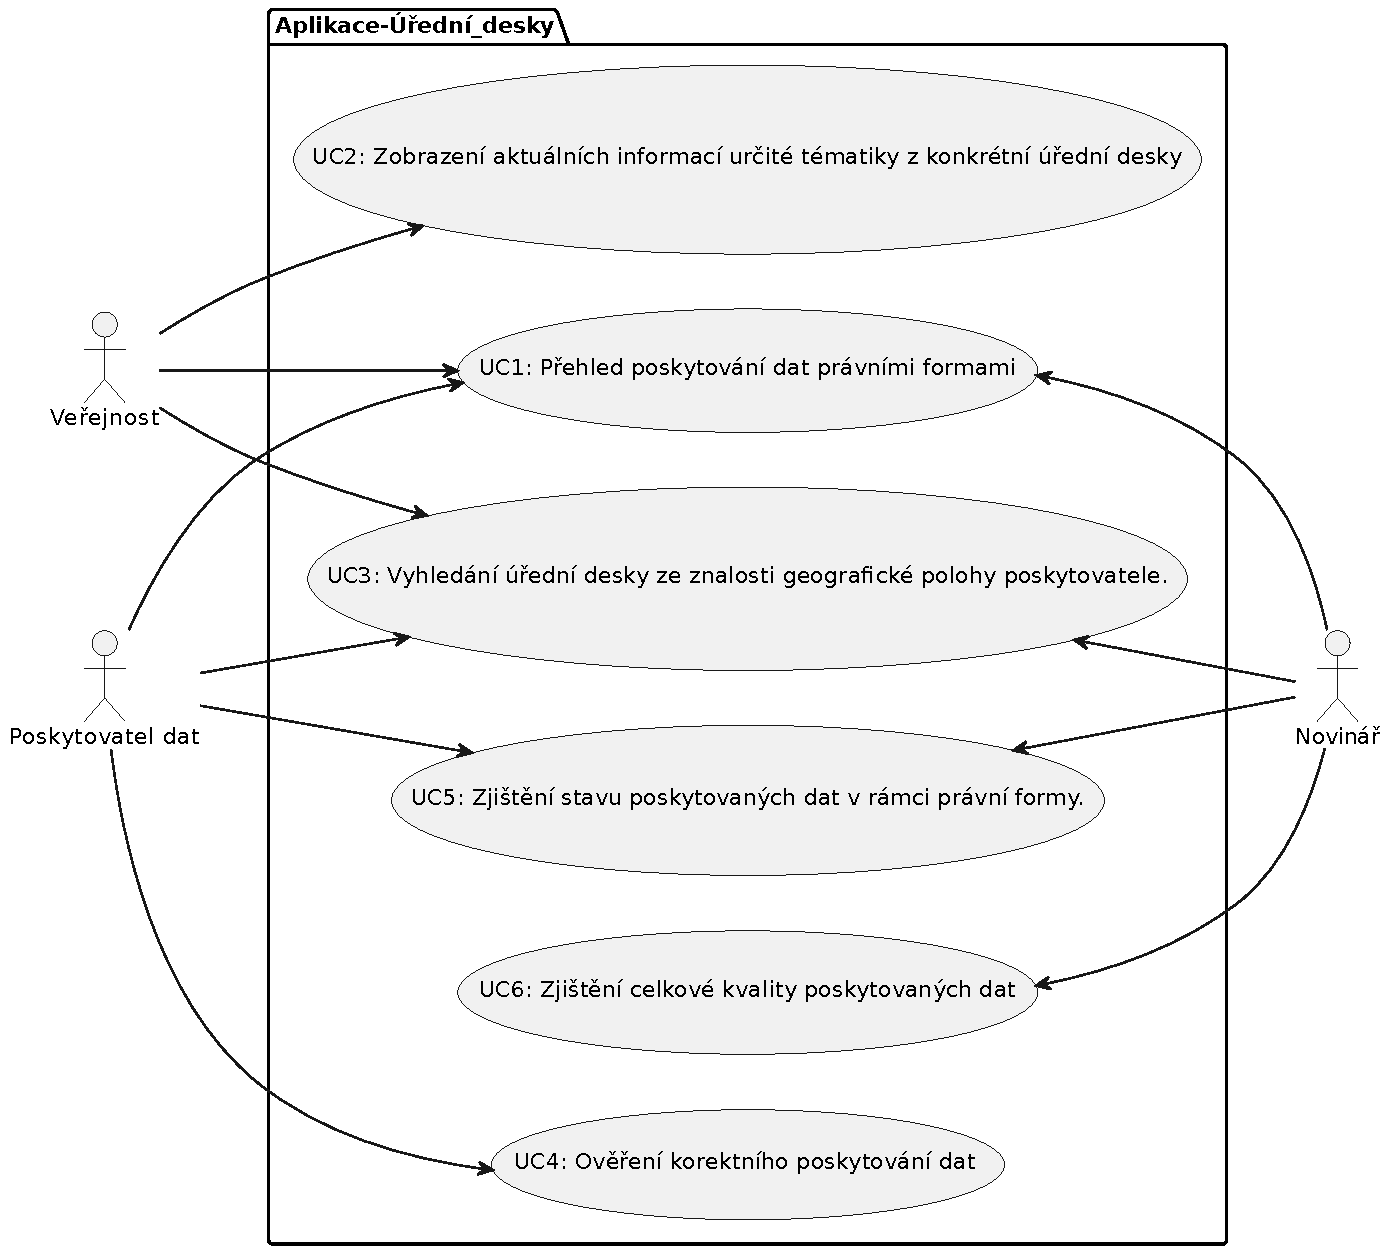
\includegraphics[width=\textwidth]{cs/obrazky/use-case-diagram.pdf}
\caption{Diagram případů užití}
\label{fig:use-case}
\end{figure}

Na obrázku \ref{fig:use-case} můžeme vidět diagram případů užití. Dále podrobně popíšeme jednotlivé případy užití.

%%%%%%%%%%%%%%%%%%%%%%%%%%%%%%%%%%%%%%%%%%%%%%%%%%%%%%%%%%%%%%

\subsection{Přehled poskytování dat právními formami}
\label{use-case:who}

Uživatel potřebuje zjistit, které orgány určité právní formy poskytují svoji úřední desku jako otevřená data. Například, které krajské úřady poskytují svoji desku.

Pokrývá požadavky: \textbf{V01}, \textbf{V03}

Role: veřejnost, poskytovatel dat, novinář

\paragraph{Počáteční stav} 
Uživatel má v aplikaci otevřený seznam úředních desek. Jsou zobrazené všechny úřední desky, které má aplikace k dispozici.

\paragraph{Normální průběh}
\begin{enumerate}
    \item Uživatel v části s filtrováním podle právních forem nechá vybranou pouze tu právní formu, která ho zajímá.
    \item Aplikace vyfiltruje pouze desky, jejichž poskytovatel má vybranou právní formu.
    \item Uživatel si prohlédne vyfiltrované úřední desky a zjistí, kteří poskytovatelé tam jsou.
\end{enumerate}

\paragraph{Odklonění od normálního průběhu}
\begin{itemize}
    \item Žádný z poskytovatelů úředních desek nemá vybranou právní formu. Aplikace zobrazí po filtrování prázdný seznam.
\end{itemize}

\paragraph{Stav po dokončení}
Uživatel zjistil, které orgány určité právní formy poskytují svoji úřední desku jako otevřená data.

%%%%%%%%%%%%%%%%%%%%%%%%%%%%%%%%%%%%%%%%%%%%%%%%%%%%%%%%%%%%%%

\subsection{Zobrazení aktuálních informací určité tématiky z konkrétní úřední desky}
\label{use-case:info}

Uživatel má zájem prohlédnout si aktuální informace, které se týkají nějakého tématu, z určité úřední desky. Může se například jednat o dražby pozemků v nějaké obci.

Pokrývá požadavky: \textbf{V02}, \textbf{V04}, \textbf{V05}, \textbf{V06}

Role: veřejnost

\paragraph{Počáteční stav} 
Uživatel má v aplikaci otevřený seznam úředních desek. Jsou zobrazené všechny úřední desky, které má aplikace k dispozici.

\paragraph{Normální průběh}
\begin{enumerate}
    \item Uživatel zadá do vyhledávání název poskytovatele úřední desky, kterou chce zobrazit. A stiskne tlačítko \texttt{Najít}.
    \item Aplikace ze všech desek vybere pouze ty, které mají hledaného poskytovatele a zobrazí je.
    \item Uživatel si vybere úřední desku, o kterou má zájem, a stiskne tlačítko \texttt{Zobrazit informace}.
    \item Aplikace získá IRI datové sady vybrané úřední desky a požadavkem do NKOD zjistí URL distribuce datové sady.
    \item Aplikace stáhne distribuci a na základě ní vizualizuje detail desky, přičemž seřadí informace od aktuálních ke starším.
    \item Uživatel zadá klíčové slovo z tématiky informace, kterou chce vyhledat (např. dražba), do vyhledávače a stiskne tlačítko \texttt{Najít}.
    \item Aplikace vyfiltruje pouze ty informace, jejichž název obsahuje dané klíčové slovo.
\end{enumerate}

\paragraph{Odklonění od normálního průběhu}
\begin{itemize}
    \item Daný poskytovatel neposkytuje svoji úřední desku jako otevřená data. Des\-ka se tedy nezobrazí při vyhledávání.
    \item Distribuci desky nelze stáhnout. Aplikace upozorní uživatele, nabídne možnost validovat desku.
    \item Úřední deska neobsahuje informace s danou tématikou. Aplikace po filtrování nezobrazí žádné informace.
\end{itemize}

\paragraph{Stav po dokončení}
Aplikace zobrazuje informace s danou tématikou z určité úřední desky.

%%%%%%%%%%%%%%%%%%%%%%%%%%%%%%%%%%%%%%%%%%%%%%%%%%%%%%%%%%%%%%

\subsection{Vyhledání úřední desky ze znalosti geografické polohy poskytovatele}
\label{use-case:mapa}

Uživatel zná geografickou polohu nějakého poskytovatele a chce najít jeho úřední desku z mapy.

Pokrývá požadavky: \textbf{V01}, \textbf{V07}

Role: veřejnost, poskytovatel dat, novinář

\paragraph{Počáteční stav} 
Uživatel má v aplikaci otevřenou mapu úředních desek. Jsou zobrazené všechny úřední desky, které má aplikace k dispozici.

\paragraph{Normální průběh}
\begin{enumerate}
    \item Uživatel na mapě vyhledá polohu poskytovatele.
    \item Uživatel vybere bod na mapě znázorňující poskytovatele, který ho zajímá a klikne na něj.
    \item Aplikace zobrazí úřední desky vybraného poskytovatele.
    \item Uživatel najde mezi zobrazenými úředními deskami tu, která ho zajímá.
\end{enumerate}

\paragraph{Odklonění od normálního průběhu}
\begin{itemize}
    \item Daný poskytovatel neposkytuje svoji úřední desku jako otevřená data. V mapě se nezobrazí bod s poskytovatelem.
\end{itemize}

\paragraph{Stav po dokončení}
Uživatel našel úřední desku v mapě podle polohy poskytovatele.

\subsection{Ověření korektního poskytování dat} \label{use-case:validace}

Uživatel v roli poskytovatele dat chce ověřit, že data z jeho úřední desky jsou zveřejněná, je možné s nimi pracovat a odpovídají specifikaci OFN pro úřední desky.

Pokrývá požadavky: \textbf{P01}, \textbf{P02}, \textbf{P03}, \textbf{P04}, \textbf{P05}, \textbf{P06}

Role: poskytovatel dat

\paragraph{Počáteční stav} 
Uživatel má v NKOD zveřejněná data z úřední desky jako otevřená data a chce provést aktualizaci datové sady. Uživatel už s aplikací pracoval a má k dispozici URL detailu svojí úřední desky, které je vytvořené z IRI datové sady v NKOD. Uživatel aktualizuje data.

\paragraph{Normální průběh}
\begin{enumerate}
    \item Uživatel otevře URL vizualizace detailu svojí úřední desky.
    \item Aplikace zobrazí vizualizaci desky.
    \item Uživatel ověří, že deska obsahuje aktualizované informace.
    \item Uživatel přejde na validační detail desky. Buď využije tlačítka \texttt{Validovat desku} ve vizualizaci, nebo přejde do sekce Validace, vyhledá desku v seznamu výsledků validace a přejde do detailu.
    \item Aplikace provede validaci a zobrazí výsledky. 
    \item Aplikace barevně zvýrazní výsledek --- zelená: validace je v pořádku, žlutá: chybí doporučené atributy, červená: nelze stáhnout distribuci.
    \item Aplikace zobrazí detaily validace --- případné chybějící atributy, nebo chybovou hlášku získanou při stahování distribuce a možné příčiny chyby.
    \item Uživatel zjistí výsledek validace svých dat.
\end{enumerate}

\paragraph{Odklonění od normálního průběhu}
\begin{itemize}
    \item Aktualizace dat změnila datovou sadu tak, že ji není možné aplikací vyhledat v NKOD (případně URL uživatele je poškozené). Aplikace zobrazí chybovou hlášku.
\end{itemize}

\paragraph{Stav po dokončení}
Uživatel ověřil, že jsou aktualizovaná data validně zveřejněná.

\subsection{Zjištění stavu poskytovaných dat v rámci právní formy} \label{use-case:statAVal}

Uživatel chce zjistit, kolik organizací nějaké právní formy poskytuje svoji úřední desku jako otevřená data a jaká je kvalita těchto dat.

Pokrývá požadavky: \textbf{P02}, \textbf{P03}, \textbf{P04}, \textbf{P07}, \textbf{N01}  

Role: poskytovatel dat, novinář

\paragraph{Počáteční stav} 
Uživatel má v aplikaci otevřenou sekci se statistikou poskytovatelů.

\paragraph{Normální průběh}
\begin{enumerate}
    \item Aplikace zobrazí pro vybrané právní formy (obsahující největší skupiny poskytovatelů) na základě dat z RPP kolik je v dané právní formě celkem organizací a kolik z nich poskytují svoji úřední desku jako otevřená data.
    \item Uživatel najde mezi právními formami tu, která ho zajímá a zjistí, jaká část organizací poskytuje svoji úřední desku.
    \item Uživatel přejde do části validace dat.
    \item Aplikace zobrazí seznam stručných výsledků validace pro všechny úřední desky.
    \item Uživatel v části s filtrováním podle právních forem nechá vybranou pouze tu právní formu, která ho zajímá.
    \item Aplikace vyfiltruje pouze výsledky validace desek, jejichž poskytovatel má vybranou právní formu.
    \item Uživatel si prohlédne výsledky validace pro vybranou kategorii.
\end{enumerate}

\paragraph{Odklonění od normálního průběhu}
\begin{itemize}
    \item V uživatelem vybrané právní formě nejsou žádní poskytovatelé dat z úředních desek. Uživatel zjistí pouze celkový počet organizací této právní formy.
\end{itemize}

\paragraph{Stav po dokončení}
Uživatel zjistil stav poskytovaných dat v rámci vybrané právní formy.

\subsection{Zjištění celkové kvality poskytovaných dat} \label{use-case:celaVal}

Uživatel chce zjistit souhrnnou kvalitu otevřených dat z úředních desek.

Pokrývá požadavky: \textbf{P02}, \textbf{P03}, \textbf{N02}  

Role: novinář

\paragraph{Počáteční stav} 
Uživatel má v aplikaci otevřenou sekci se statistikou validace.

\paragraph{Normální průběh}
\begin{enumerate}
    \item Aplikace zobrazí provede validaci všech distribucí úředních desek.
    \item Aplikace zobrazí uživateli následující údaje: kolik distribucí se podařilo (nepodařilo) stáhnout, kolika distribucím chybí některé doporučené atributy. Výsledky zobrazí v textové podobě a procentuálně na koláčovém grafu.
    \item Uživatel si prohlédne souhrnné výsledky validace.
\end{enumerate}

\paragraph{Stav po dokončení}
Uživatel zjistil souhrnnou kvalitu otevřených dat z úředních desek.



\chapter{Návrh aplikace}\label{kap:navrh}

V této kapitole se zabýváme návrhem aplikace. Popíšeme moduly, ze kterých se aplikace skládá a jejich uživatelská rozhraní. Dále popíšeme architekturu aplikace, její vnitřní strukturu a to, jak je napojená na externí systémy a jak získává data.

\section{Moduly}\label{sec:moduly}

Na základě požadavků popsaných v kapitole \ref{kap:pozadavky} můžeme funkcionality aplikace rozdělit do tří hlavních modulů: Vizualizace, Validace a Statistika.

\subsection{Vizualizace}

Modul Vizualizace bude odpovídat za zobrazování úředních desek a informací na nich. 

\subsubsection{Seznam úředních desek}

\begin{figure} 
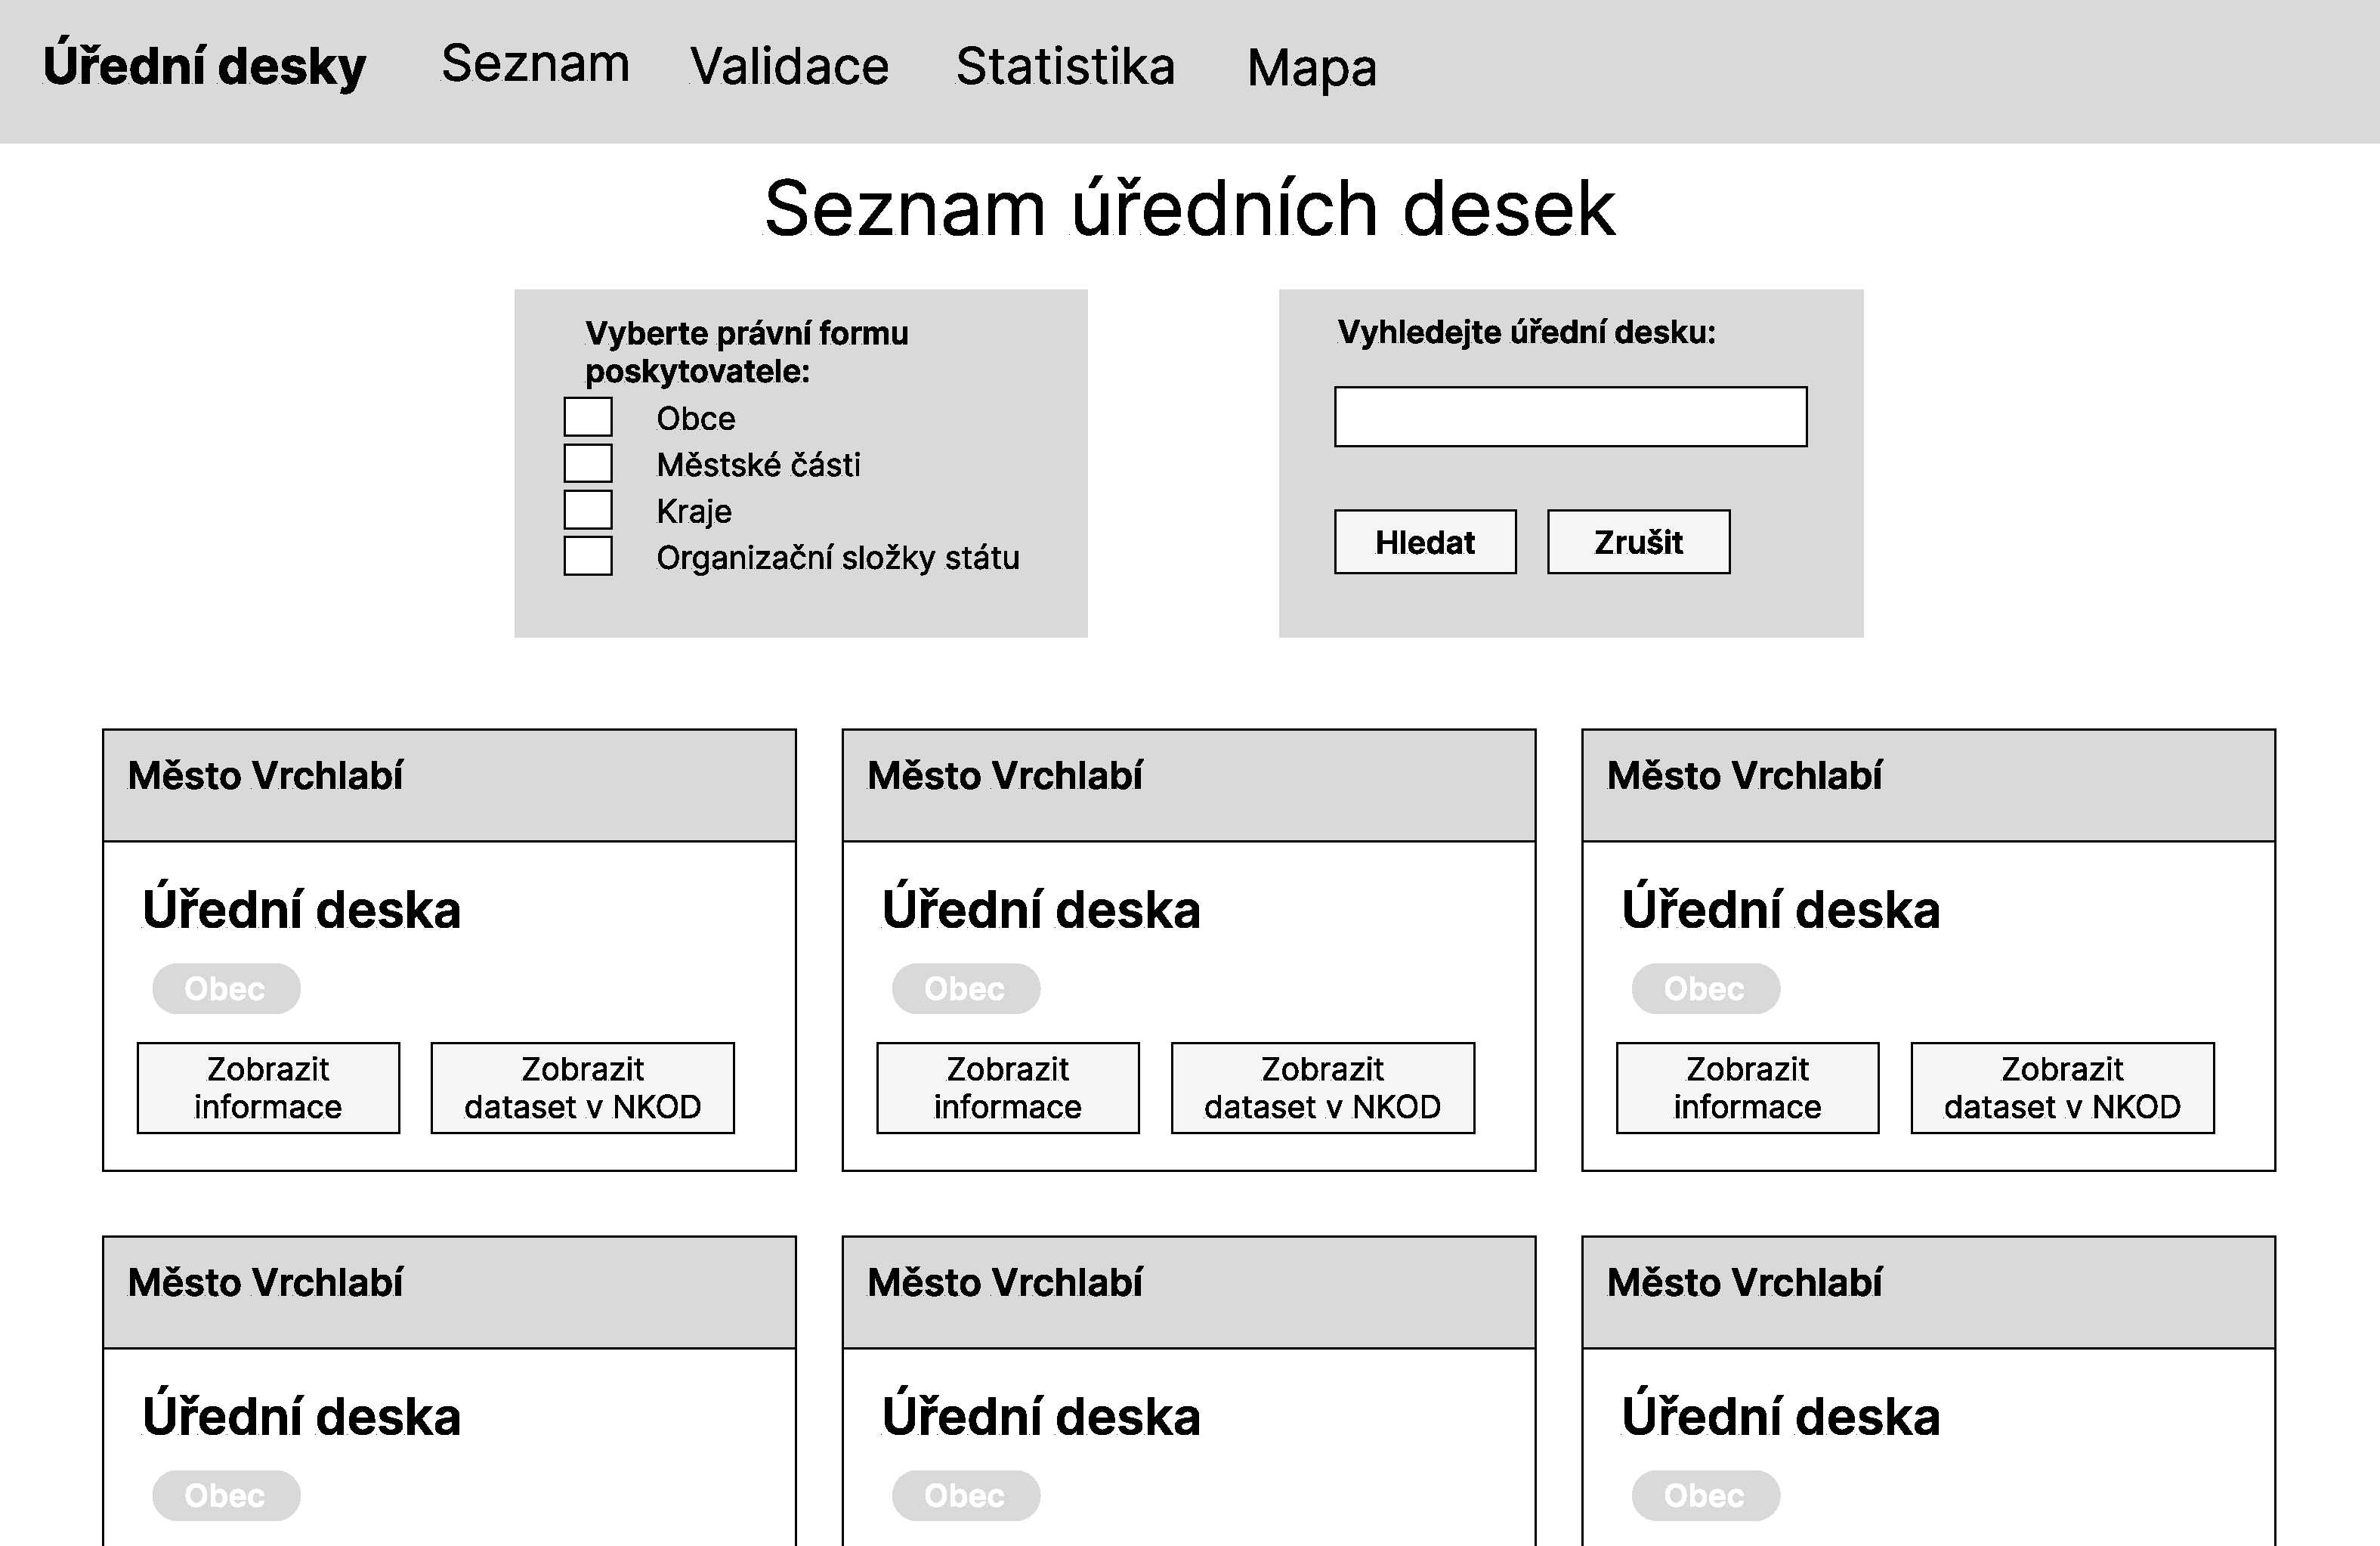
\includegraphics[width=1\textwidth, frame]{cs/obrazky/wireframes/wireframe_seznam.pdf}
\caption{Návrh uživatelského rozhraní - Seznam úředních desek}
\label{fig:seznam}
\end{figure}

Podle požadavku \textbf{V01} aplikace bude zobrazovat seznam všech úředních desek zveřejněných v NKOD podle OFN pro úřední desky. Pro reprezentaci úřední desky v seznamu je možné použít metadata, která získáme z NKOD při získání datové sady úřední desky, tedy název desky a název poskytovatele. Používáme pouze tato data, abychom mohli zobrazit seznam úředních desek bez nutnosti stahovat distribuce všech desek.

V seznamu bude možné vyhledat úřední desku podle názvu poskytovatele nebo názvu desky (požadavek \textbf{V02}). Bude k tomu sloužit formulář pro hledání. 

Modul dále umožní filtrování úředních desek podle právní formy poskytovatele (požadavek \textbf{V03}). Při analýze dat jsme objevili 4 hlavní právní formy poskytovatelů dat:
\begin{itemize}
    \item obce
    \item městské části a městské obvody
    \item kraje
    \item organizační složky státu
\end{itemize}
Pro tyto kategorie bude aplikace podporovat filtrování desek. Organizace jiných právních forem buď svoje úřední desky neposkytují, nebo se jedná o nižší jednotky desek, proto jsme pro ně vytvořili souhrnnou kategorii ostatní. Do této kategorie spadá i několik úředních desek poskytovatelů, kteří v RPP nemají uvedenou svoji právní formu, aplikace ji tedy nemůže zjistit.

Úřední desky v seznamu budou pro odlišení toho, do které spadají kategorie, obsahovat označení právní formy poskytovatele. Dále budou obsahovat odkaz na datovou sadu dané úřední desky v NKOD, jako možnost prohlédnout si syrová data z úřední desky, a také odkaz na vizualizaci informací na dané úřední desce (požadavek \textbf{V04}).

Na obrázku \ref{fig:seznam} najdeme návrh uživatelského rozhraní pro seznam úředních desek. V horní části obrazovky je umístěný navigační panel, pomocí kterého je možné přepínat mezi jednotlivými částmi aplikace. Dále na stránce najdeme dva formuláře, levý slouží pro filtrování a pravý pro vyhledávání úředních desek. Pod formuláři následuje seznam úředních desek, kde každá deska je reprezentovaná jednou kartičkou.



Seznam úředních desek je stránkovaný. Při načtení se zobrazí pouze prvních 20 desek. Ostatní desky je možné zobrazit zmáčknutím tlačítka \textit{Zobrazit další}, což přidá dalších 20 desek, nebo je možné načíst všechny desky zmáčknutím tlačítka \textit{Zobrazit vše}. Tato tlačítka jsou umístěná ve spodní části stránky, jejich návrh můžeme vidět na obrázku \ref{fig:paging}.

\begin{figure} 
\begin{center}
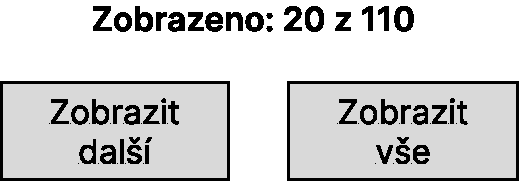
\includegraphics[width=0.3\textwidth]{cs/obrazky/wireframes/wireframe_paging.pdf} 
\end{center}
\caption{Návrh uživatelského rozhraní - Stránkování}
\label{fig:paging}
\end{figure}

\subsubsection{Detail úřední desky}

V detailu úřední desky bude možné si prohlédnout informace zveřejněné na této úřední desce (požadavek \textbf{V04}). Pro detail úřední desky použijeme data z distribuce datové sady, tedy metadata desky a informací, která odpovídají OFN pro úřední desky. Detail úřední desky bude obsahovat:
\begin{itemize}
    \item název desky
    \item název poskytovatele dat v NKOD
    \item název provozovatele desky, který je uveden v distribuci
    \item seznam všech informací na úřední desce setříděný podle data vyvěšení (požadavek \textbf{V05})
\end{itemize}

Každá informace v detailu desky bude mít následující položky (pokud jsou tyto položky přítomné v distribuci desky): 
\begin{itemize}
    \item název informace
    \item datum vyvěšení
    \item datum, do kterého je informace relevantní
    \item odkaz na obsah informace na elektronické stránce dané úřední desky
    \item přílohy (pokud má)
\end{itemize}

V informacích bude možné vyhledávat pomocí formuláře obdobného jako při vyhledávání úředních desek v seznamu. Hledání budeme provádět na základě názvu informace (požadavek \textbf{P06})

Podle požadavku \textbf{P01} bude možné k detailu konkrétní desky přistoupit pomocí IRI datové sady, umístěním IRI do query parametru \uv{iri} v URL aplikace.

\begin{figure} 
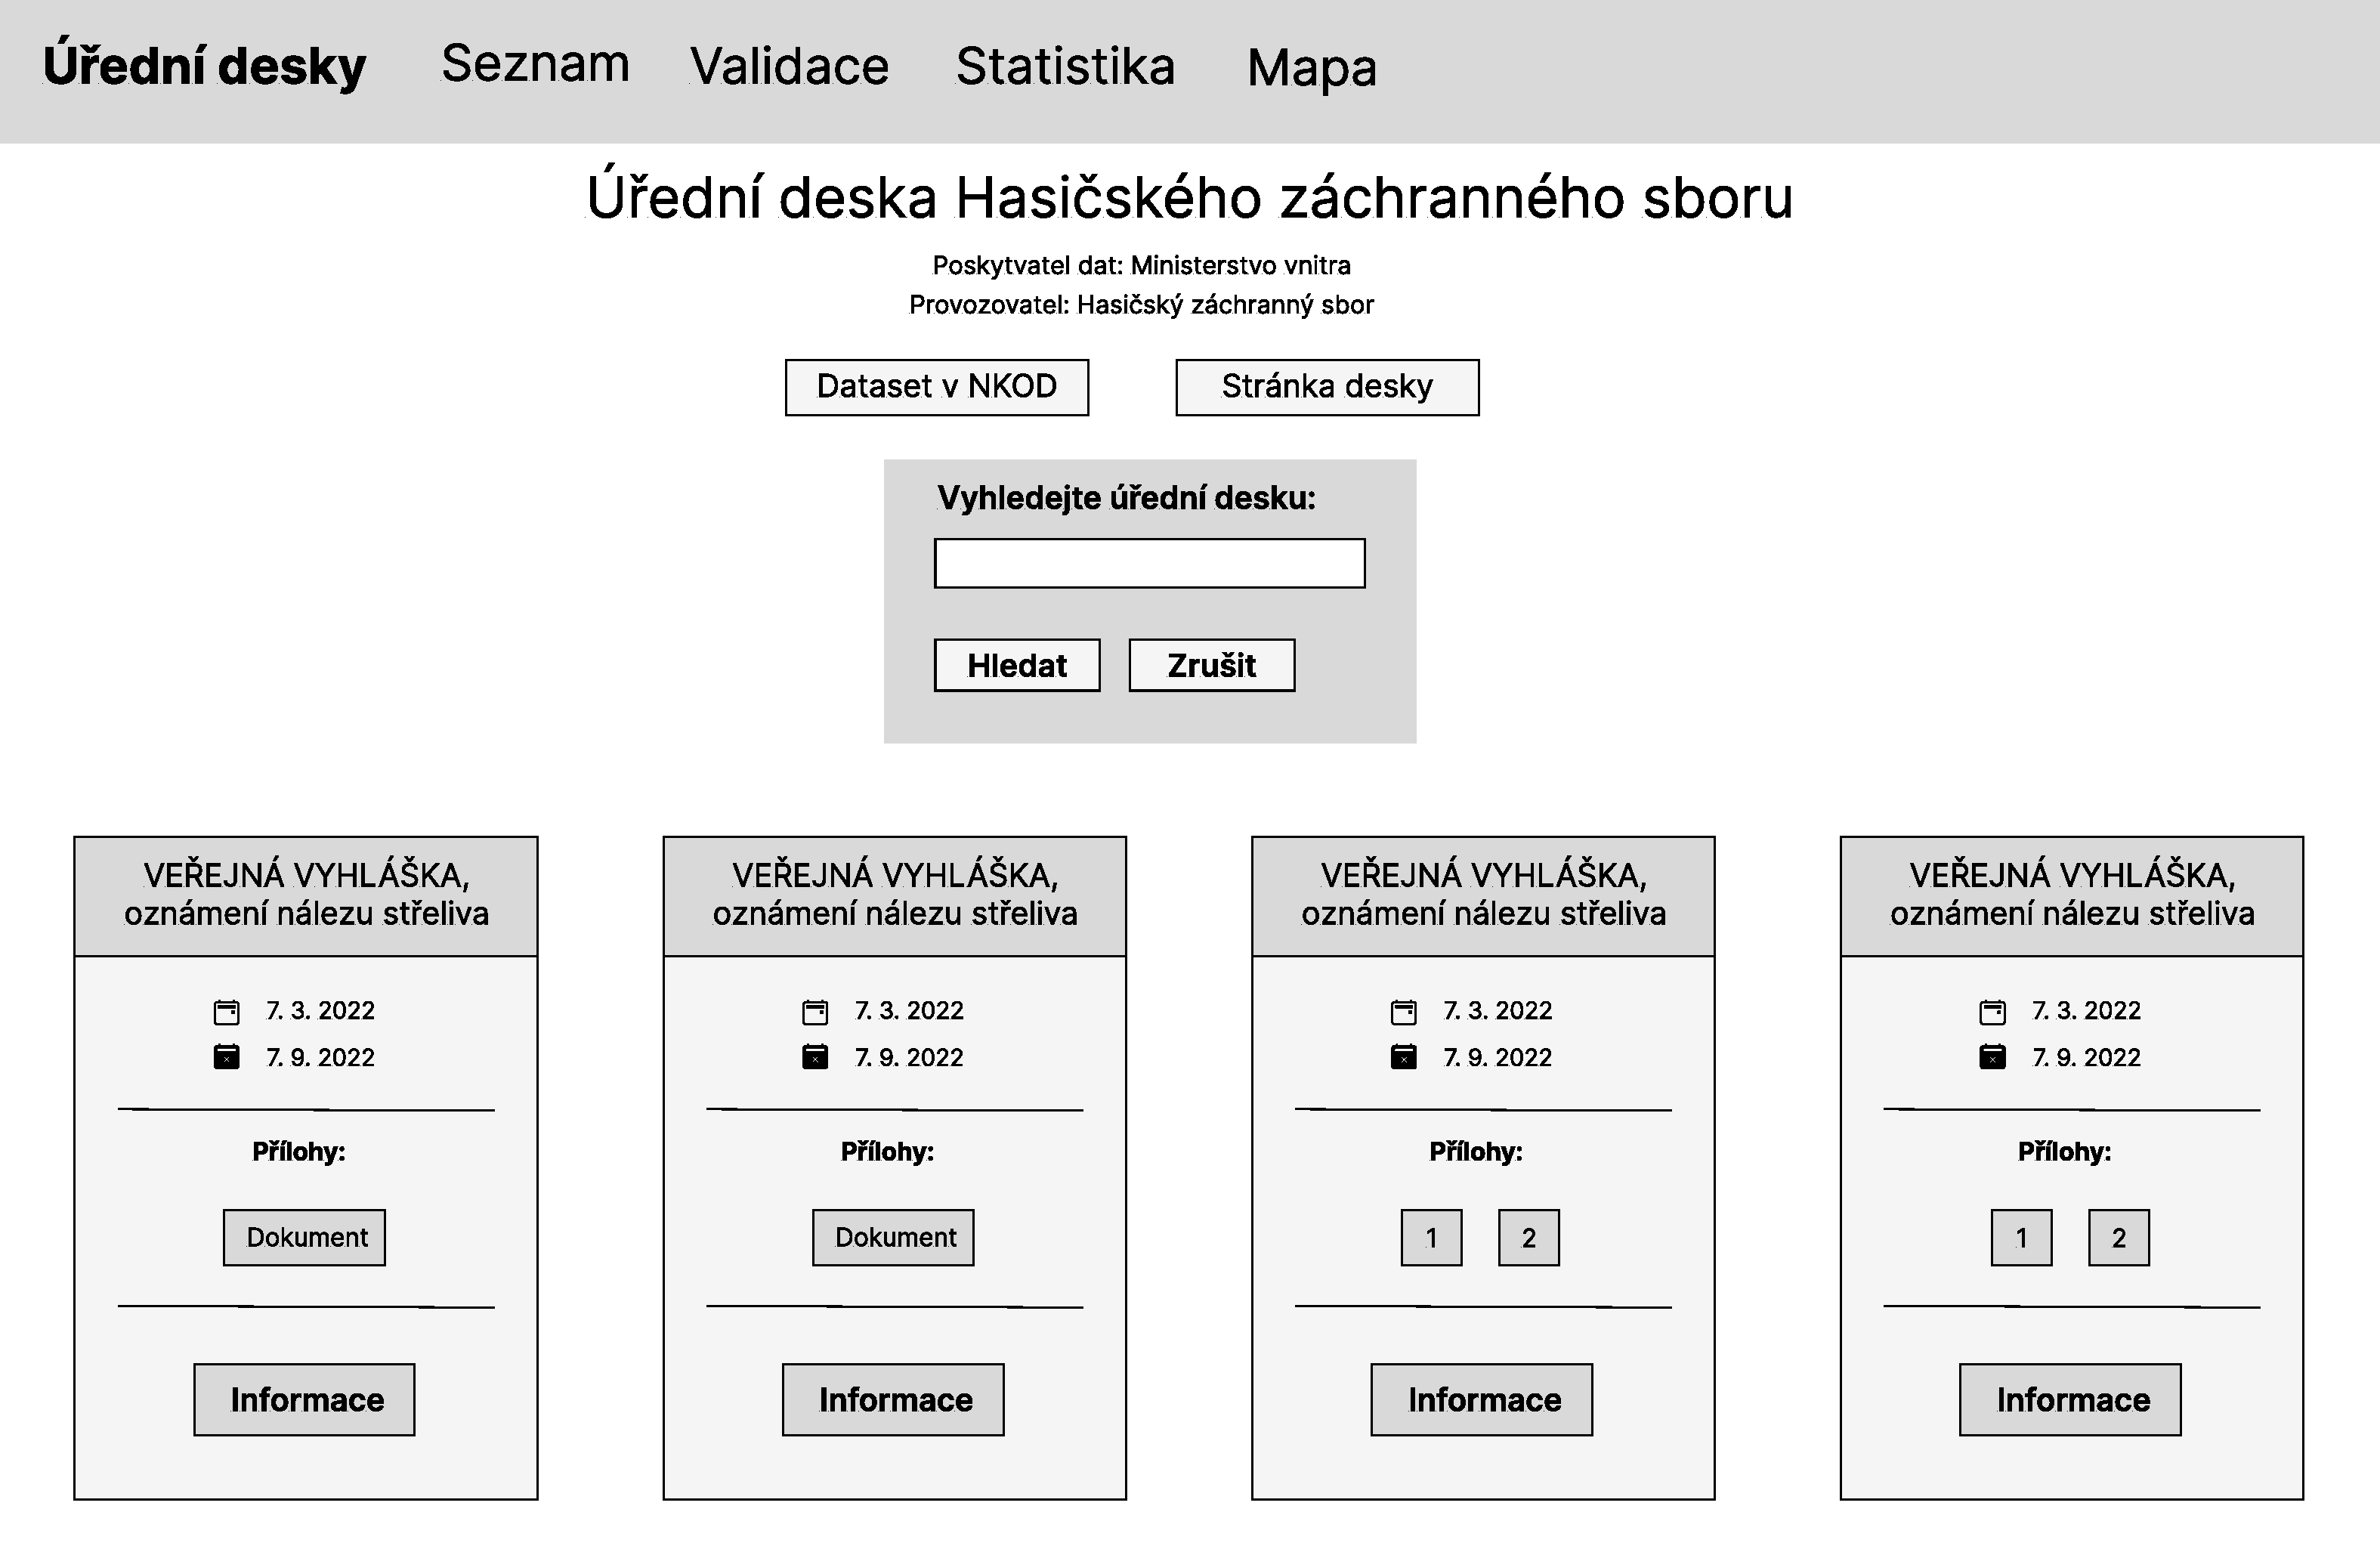
\includegraphics[width=\textwidth, frame]{cs/obrazky/wireframes/wireframe_detail.pdf}
\caption{Návrh uživatelského rozhraní - Detail úřední desky}
\label{fig:detail}
\end{figure}

\begin{figure} 
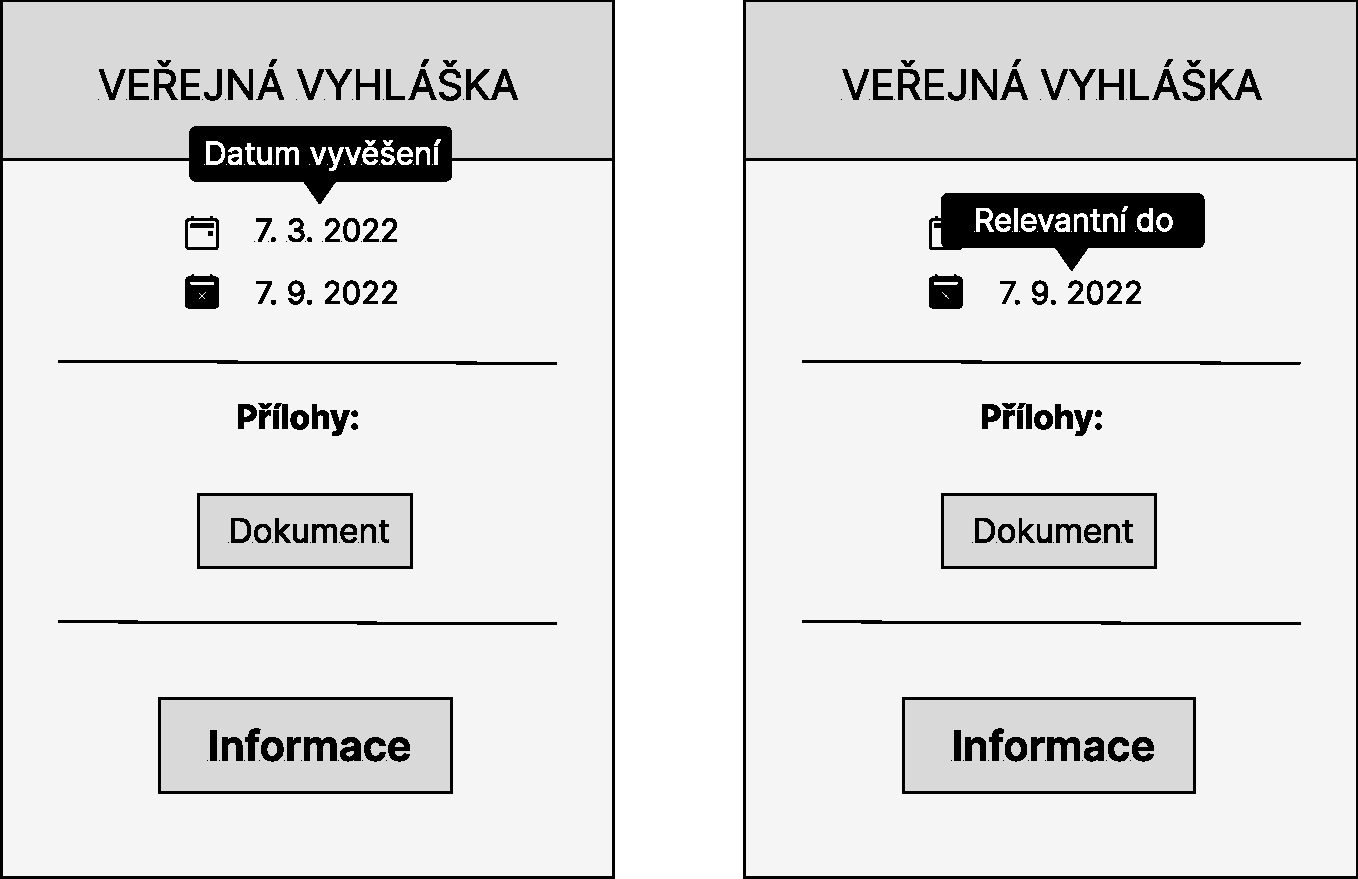
\includegraphics[width=1\textwidth]{cs/obrazky/wireframes/wireframe_detail_datum.pdf}
\caption{Návrh uživatelského rozhraní - Data platnosti informace - popisky}
\label{fig:detail-datum}
\end{figure}

Na obrázku \ref{fig:detail} vidíme návrh uživatelského rozhraní pro detail úřední desky. Na obrázku najdeme formulář pro vyhledání úřední desky a kartičky, které představují jednotlivé informace. Na kartičkách si všimneme dvou způsobů, kterými jsou zobrazeny přílohy informace. Pokud má informace pouze jednu přílohu, zobrazíme ji jako tlačítko s nápisem \textit{Dokument} (první dvě informace), pokud má příloh více, zobrazíme je jako očíslovaná tlačítka (druhé dvě informace). Tlačítko \textit{Informace} vede na URL, na kterém je informace zveřejněná.

V horní části kartičky s informací jsou dvě data --- datum vyvěšení a datum skončení relevance. Pro jejich znázornění jsme zvolili ikony, aby se textové popisky dat na kartičkách příliš neopakovaly. Pro větší přehlednost se při najetí myší na datum zobrazí jeho popisek, jak je vidět na obrázku \ref{fig:detail-datum}



Informace v detailu desky jsou stránkované stejným způsobem, jako kartičky s deskami v seznamu úředních desek.

\subsubsection{Mapa úředních desek}

\begin{figure} 
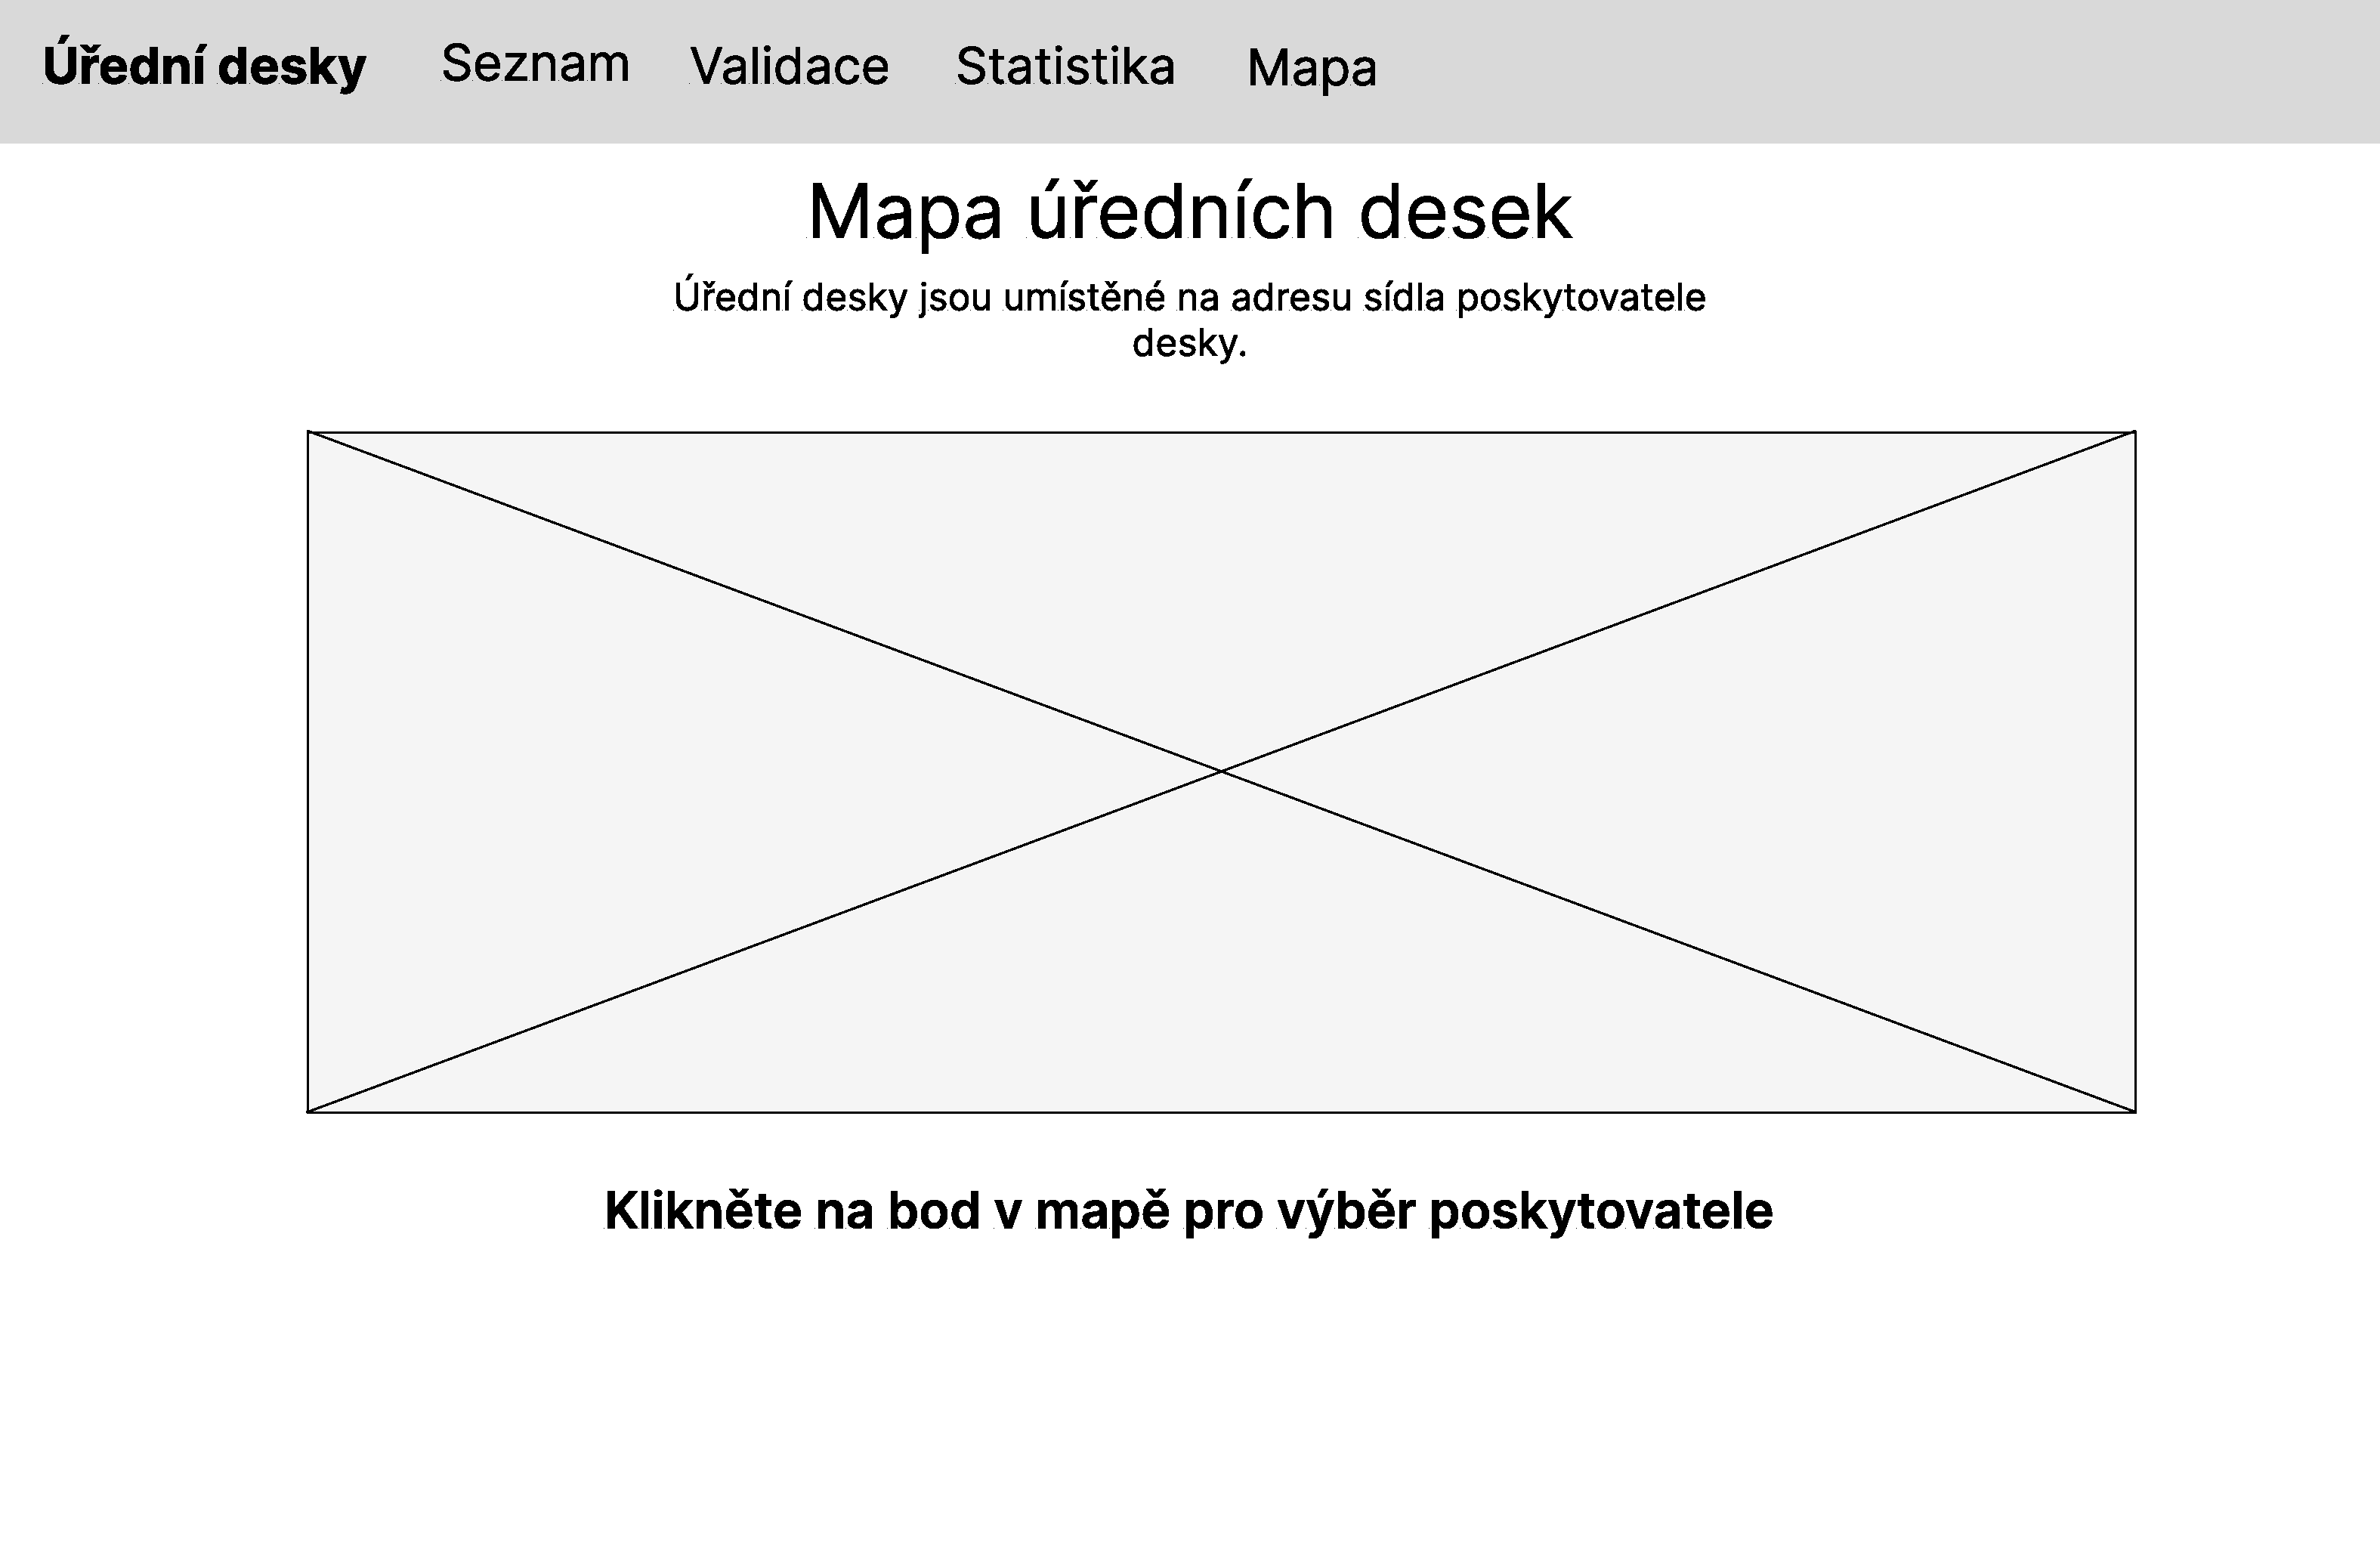
\includegraphics[width=\textwidth, frame]{cs/obrazky/wireframes/wireframe_mapa.pdf}
\caption{Návrh uživatelského rozhraní - Mapa úředních desek}
\label{fig:mapa}
\end{figure}

Kromě vizualizace úředních desek v podobě seznamu bude modul také nabízet vizualizaci na mapě (požadavek \textbf{V07}). Mapa bude po načtení přiblížená tak, aby ukazovala mapu ČR. Na mapě budou zobrazené body, reprezentující poskytovatele úředních desek. Body budou umístěné na souřadnice adresy sídla poskytovatele získané z RPP. Při kliknutí na bod v mapě se zobrazí všechny úřední desky, které daný poskytovatel zveřejňuje. Body budou barevně odlišené podle právní formy poskytovatele.

Na obrázku \ref{fig:mapa} vidíme návrh uživatelského rozhraní mapy úředních desek.


\subsection{Validace}

Modul Validace obsahuje všechny funkcionality, které se týkají validace dat z úředních desek. Cílem validace je ověřit, že distribuce dané úřední desky obsahuje všechny doporučené atributy podle specifikace OFN (požadavky \textbf{P02} a \textbf{P03}). V případě, že distribuci úřední desky nelze stáhnout, aplikace na to uživatele upozorní a nabídne možná řešení.

Nabízená řešení vychází z analýzy příčin způsobujících chyby při stahování. Objevili jsme následující příčiny (příčiny jsou seřazené od nejčastějších):
\begin{enumerate}
    \item Špatné nastavení hlavičky \uv{Access-Control-Allow-Origin}, kdy je distribuce desky správně zveřejněná, ale není možné ji stáhnout strojově požadavkem z kódu.
    \item URL distribuce uvedené v NKOD je neplatné, nebo nevede na soubor s distribucí.
    \item Neplatný SSL certifikát stránky.
\end{enumerate}
Aplikace tedy uživatele upozorní na uvedené 3 příčiny a nabídne odkazy na další informace.

Strukturou je modul Validace podobný modulu Vizualizace. Obsahuje seznam stručných výsledků validací úředních desek a detail validace pro každou desku. Seznam je možné filtrovat podle typu poskytovatele a vyhledávat v něm (požadavky \textbf{P06} a \textbf{P07}).  V seznamu je pro každou desku zobrazeno stručné shrnutí validace:
\begin{itemize}
    \item je možné stáhnout distribuci (ano/ne)
    \item metadata celé desky obsahují všechny doporučené atributy (ano/ne)
    \item metadata všech informací na desce obsahují všechny doporučené atributy (ano/ne)
    \item celkový počet informací na desce
\end{itemize}
Ze shrnutí je možné otevřít detail validace desky.

Rozhodli jsme se, že seznam výsledků validace budeme zobrazovat v tabulce. Výsledky validace mají charakter tabulkových dat, kdy jsou pro každou úřední desku zobrazeny hodnoty v několika kategoriích, proto je zobrazení tabulkou pro tato data přirozenou a přehlednou volbou. 

Nevýhodou tabulky je její špatná přizpůsobivost užším obrazovkám, jako jsou mobilní zařízení. Nicméně jsme usoudili, že uživatel s rolí poskytovatel dat, bude nejspíše aplikaci používat v rámci pracovní doby na počítači, tedy je zde tabulka vhodná. Při otevření aplikace na úzkém displeji zobrazíme uživateli upozornění, že je lepší tento modul aplikace prohlížet na širším displeji.

Na obrázku \ref{fig:validace} vidíme návrh uživatelského rozhraní pro tabulku s přehledem validace. Řádky tabulky jsou barevně zvýrazněné podle výsledku validace dané úřední desky --- červeně, pokud nelze stáhnout distribuci a žlutě, pokud chybí některé doporučené atributy.

\begin{figure} 
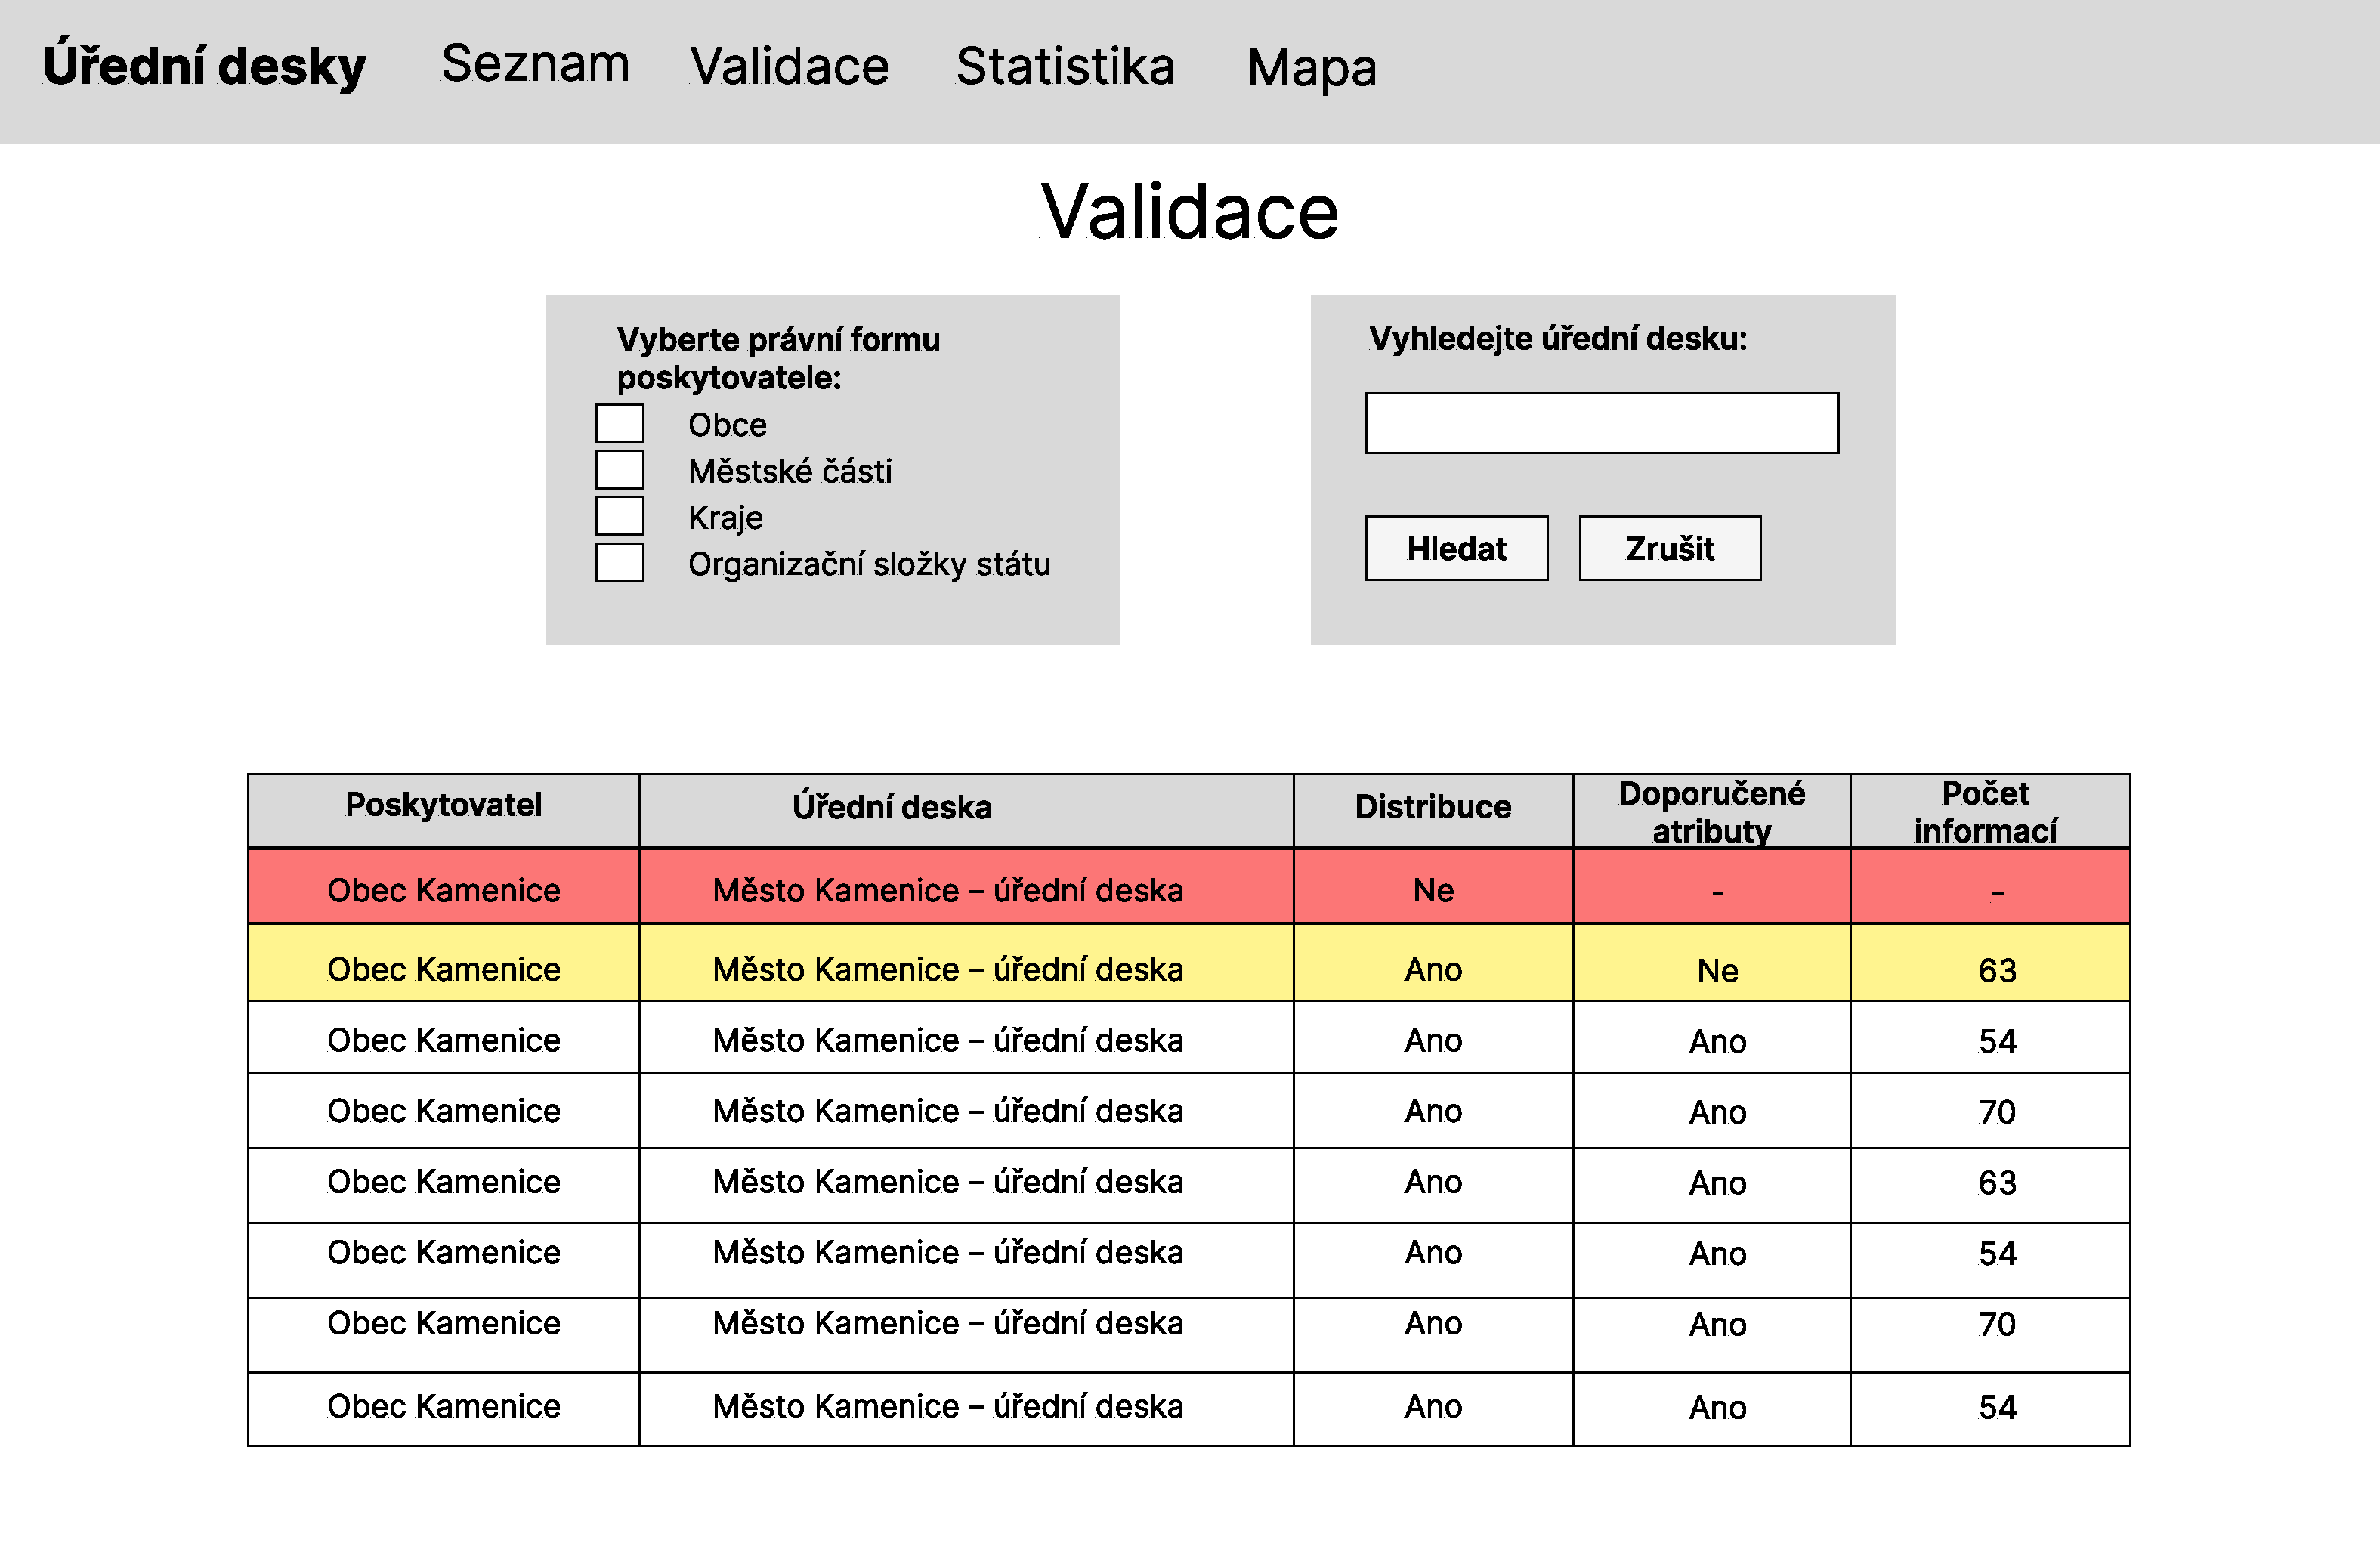
\includegraphics[width=\textwidth, frame]{cs/obrazky/wireframes/wireframe_validace.pdf}
\caption{Návrh uživatelského rozhraní - Přehled validace}
\label{fig:validace}
\end{figure}

Řádky tabulky s výsledky validace jsou stránkované stejným způsobem jako úřední desky v seznamu úředních desek.

\subsubsection{Detail validace úřední desky}

Na obrázku \ref{fig:validace-detail} je návrh uživatelského rozhraní pro detail validace úřední desky.

\begin{figure} 
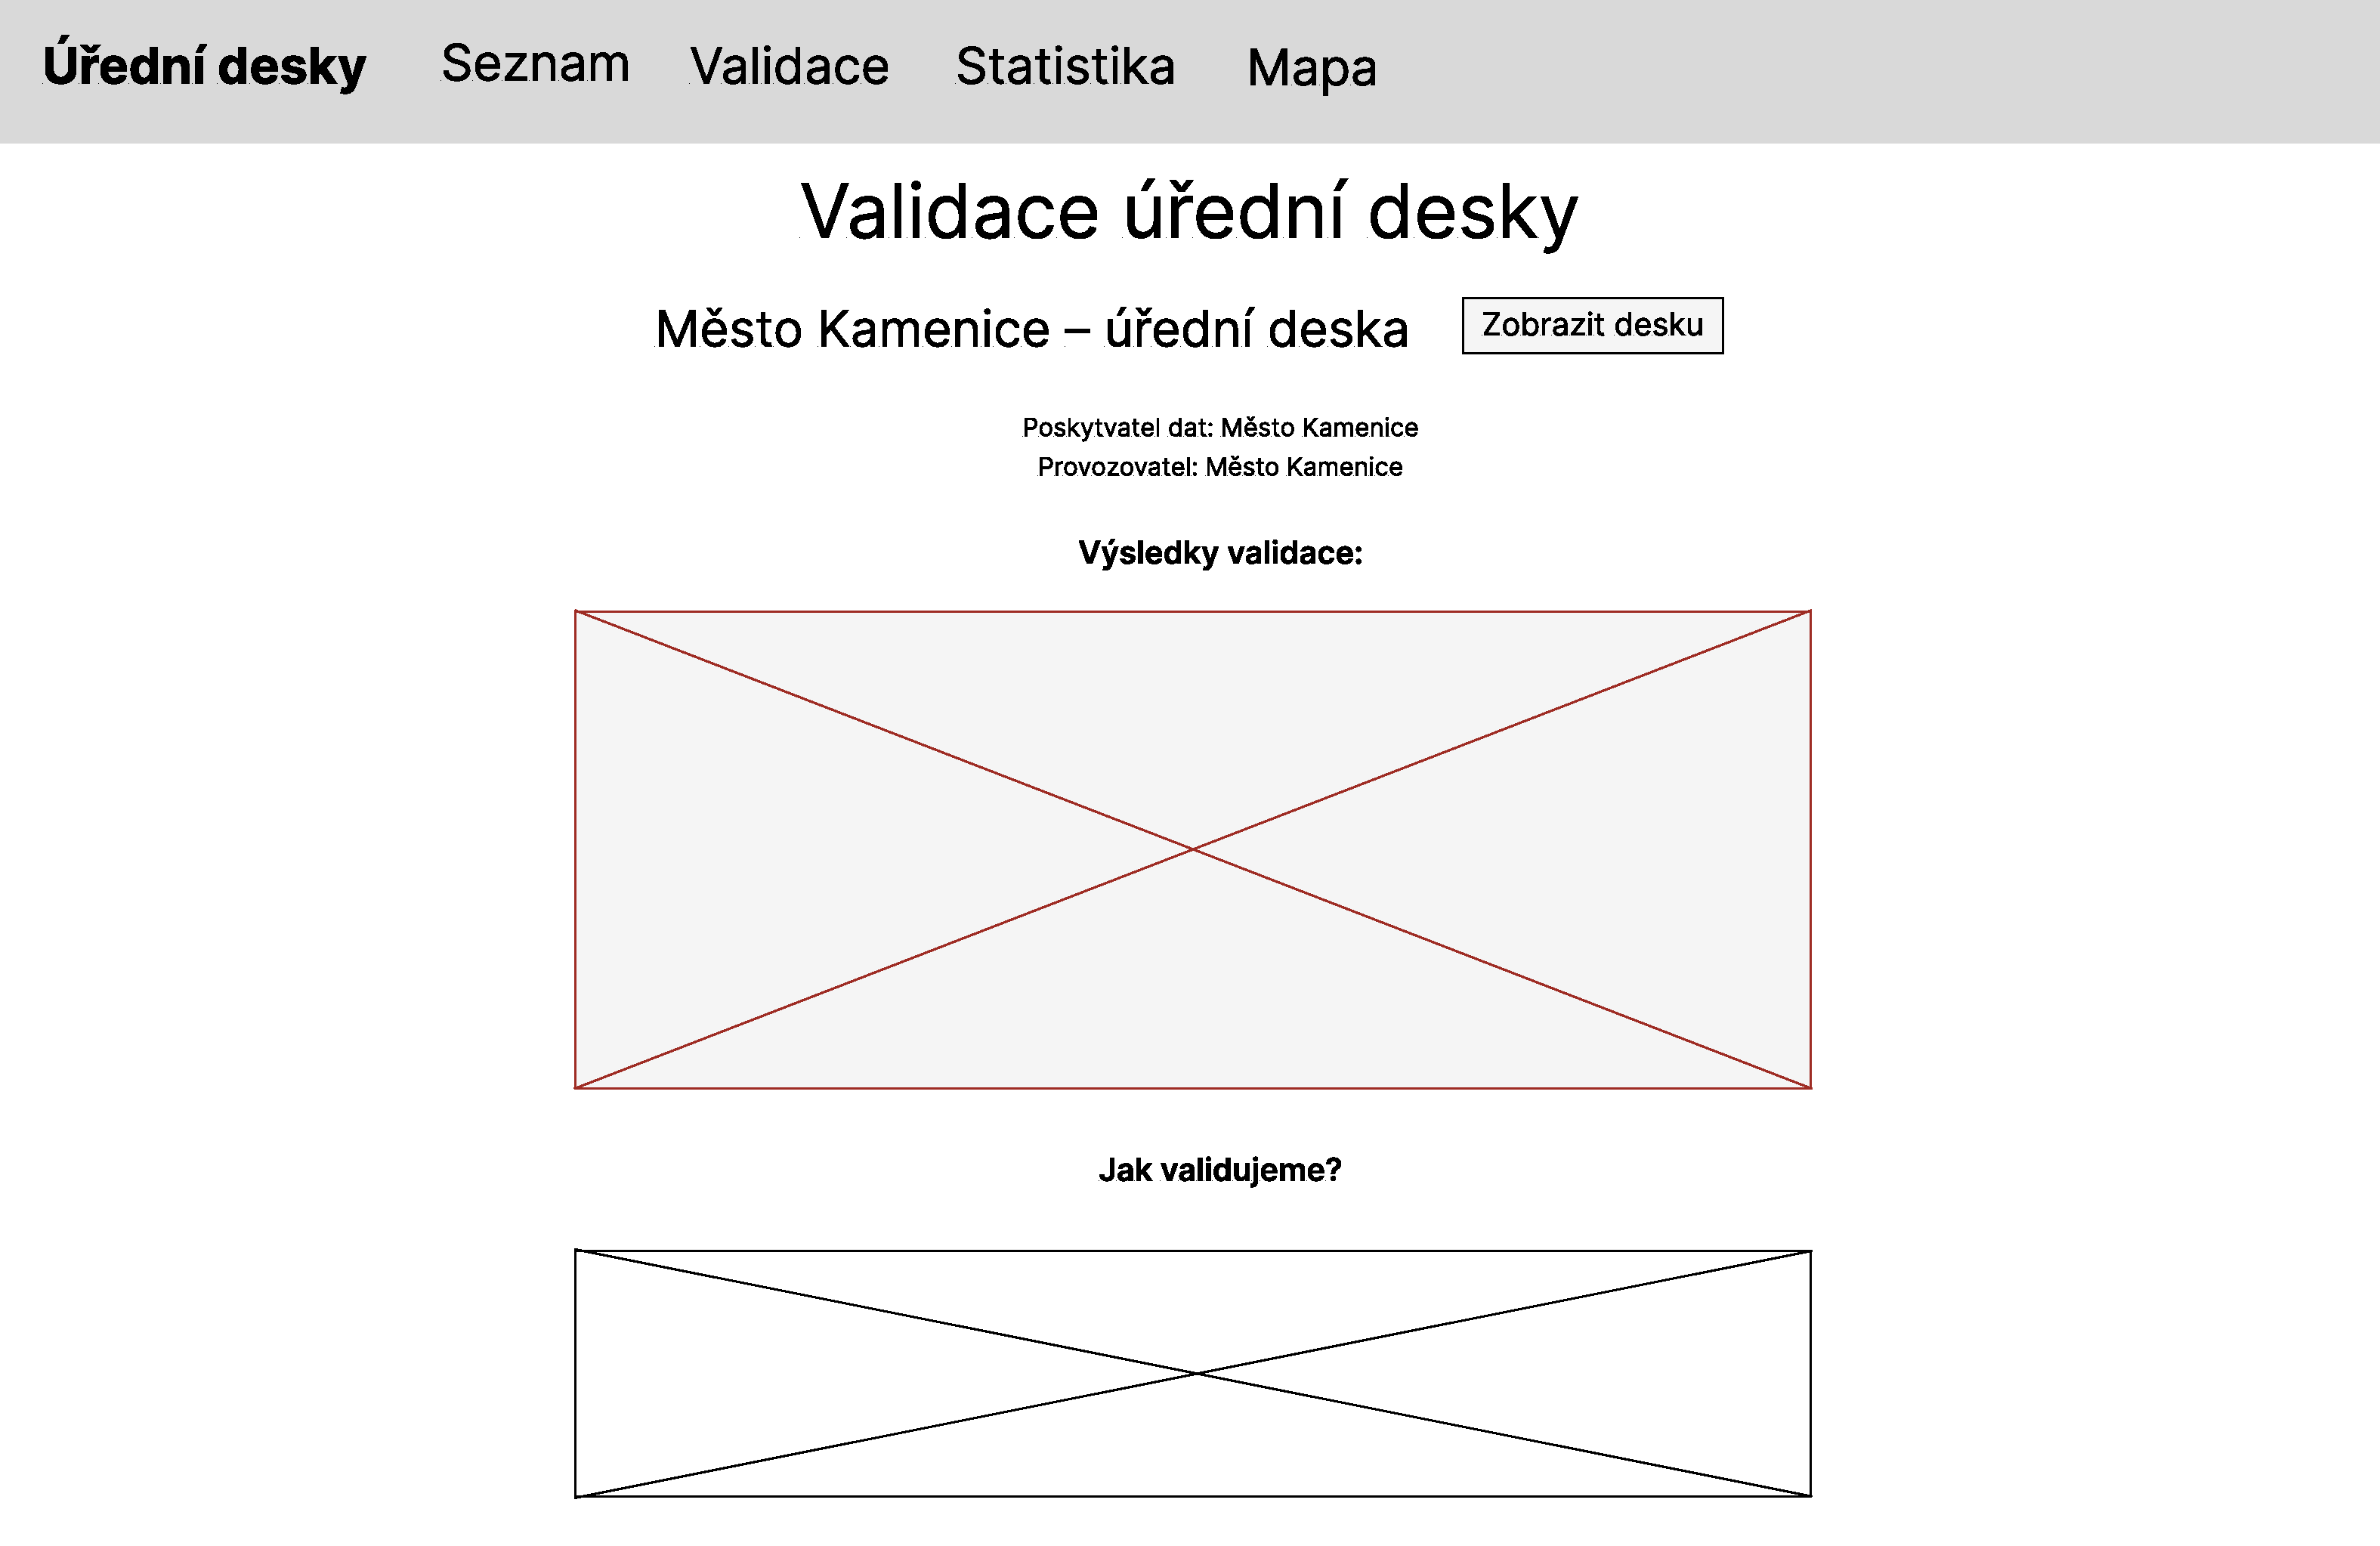
\includegraphics[width=\textwidth, frame]{cs/obrazky/wireframes/wireframe_validace_detail.pdf}
\caption{Návrh uživatelského rozhraní - Detail validace}
\label{fig:validace-detail}
\end{figure}

V horní části najdeme název úřední desky a odkaz na vizualizaci desky, a také informace o poskytovateli a provozovateli desky. Dále je na stránce umístěn rámeček s výsledkem validace, který je barevně označený podle výsledku.

Pro úřední desku, jejíž distribuci nelze stáhnout se v rámečku zobrazí upozornění, které obsahuje URL distribuce, chybová hláška získaná z nepovedeného dotazu na stažení distribuce a možná řešení problému popsaná výše. Rámeček má červenou barvu.

Pro úřední desku, kde chybí některé doporučené atributy, je rámeček žlutý. Je v něm vypsáno, které atributy chybí. V případě, že chybí doporučené atributy v metadatech informace, jsou zobrazeny všechny informace, kde chybí atributy a u každé informace je uvedeno, o které atributy se jedná. 

Pokud distribuce úřední desky nemá nedostatky, obsahuje rámeček jenom krátkou informaci o úspěšné validaci a je zelený.

Na obrázku \ref{fig:validace-detail} je ukázaný případ, kdy distribuci desky není možné stáhnout.

V každém případě detail validace kromě výsledku validace nabízí i vysvětlení, jak se validuje, kde jsou popsané jednotlivé doporučené atributy a jejich význam v datech. Toto vysvětlení je v návrhu na obrázku  \ref{fig:validace-detail} umístěné místo rámečku pod nadpisem \textit{Jak validujeme?}.


\subsection{Statistika}

Modul Statistika se věnuje zobrazení statistik z validace dat a statistik poskytovatelů podle požadavků \textbf{N01} a \textbf{N02}. 

\subsubsection{Statistika validace}

Část, která se týká validace dat, bude obsahovat souhrnný stav validace v textovém popisu a na koláčovém grafu. Statistika bude složená z následujících údajů:
\begin{itemize}
    \item Celkový počet úředních desek zveřejněných jako otevřená data.
    \item Počet distribucí desek, které nebylo možné stáhnout.
    \item Počty desek, které neobsahují všechny doporučené atributy, rozdělené podle toho, kterým chybí atributy celé desky a atributy jednotlivých informací.
    \item Celkový počet desek s nedostatky (nestažitelná distribuce, chybějící atributy).
\end{itemize}

Tato část bude také obsahovat seznam všech desek s nedostatky. Pro každou desku v seznamu bude možné otevřít detail její validace v modulu Validace.

Na obrázku \ref{fig:stat-validace} je zobrazen návrh uživatelského rozhraní pro statistiku validace.

\begin{figure} 
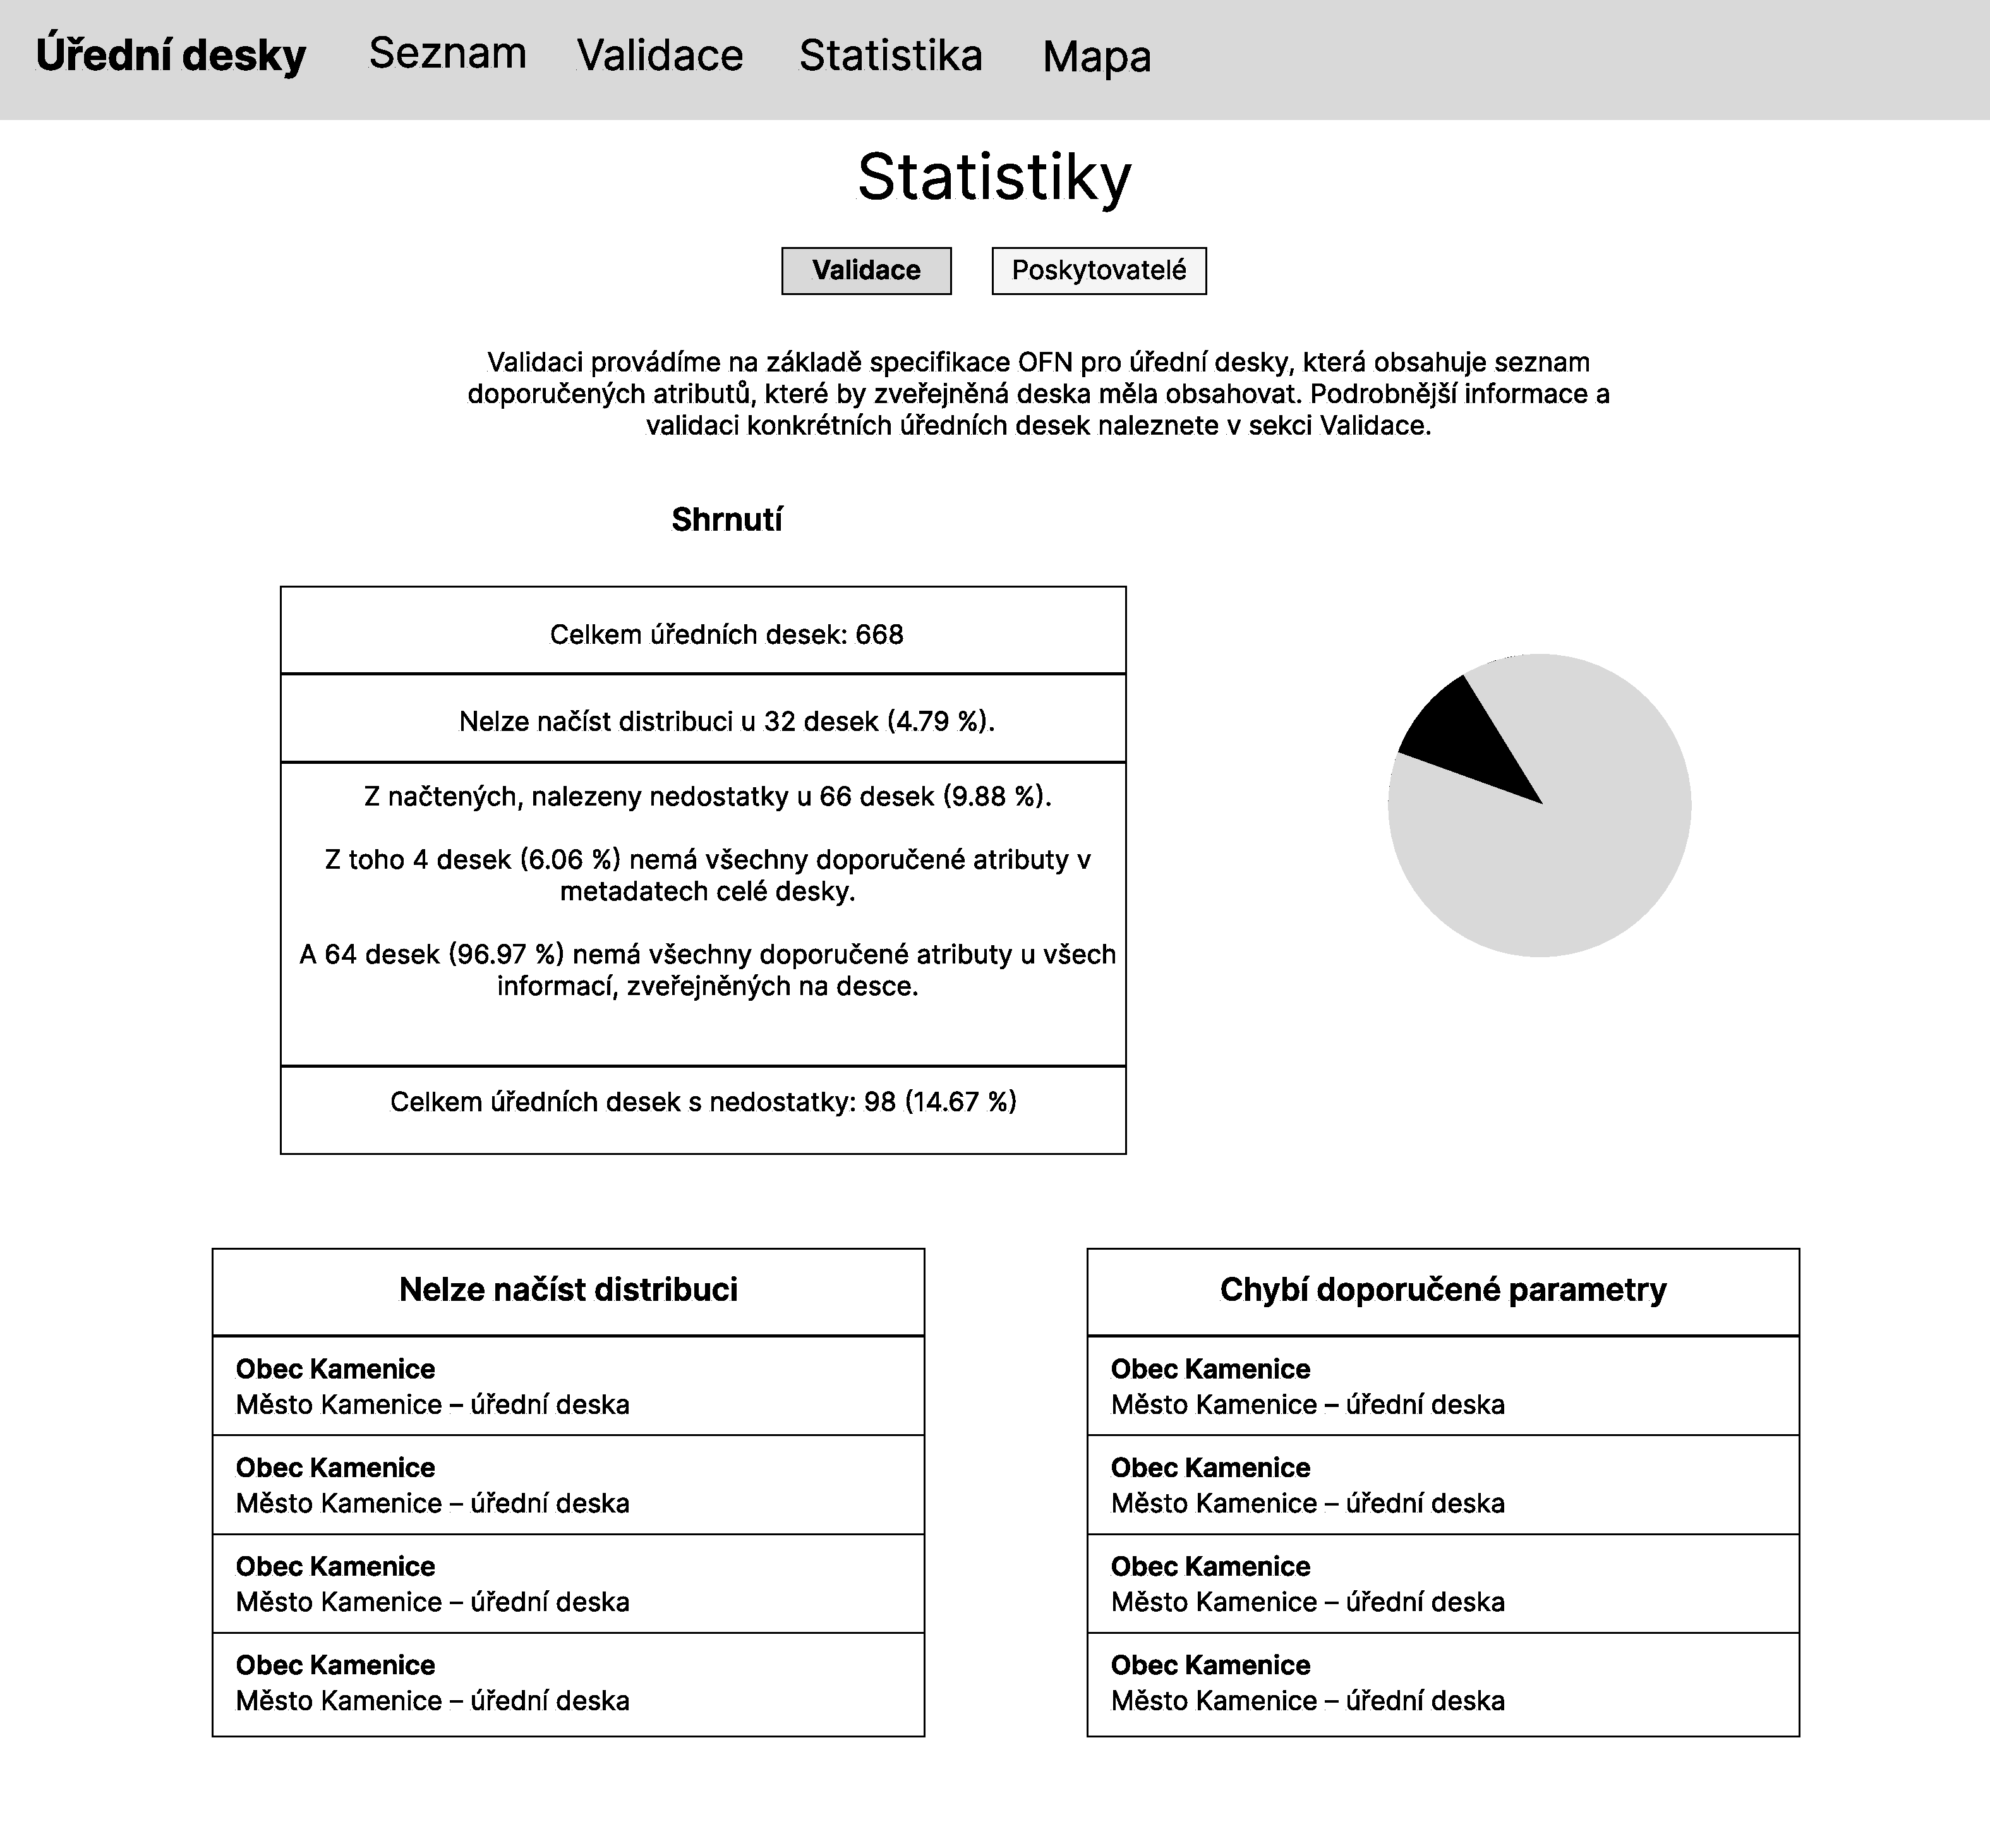
\includegraphics[width=\textwidth, frame]{cs/obrazky/wireframes/wireframe_statistika_validace.pdf}
\caption{Návrh uživatelského rozhraní - Statistika validace}
\label{fig:stat-validace}
\end{figure}

\subsubsection{Statistika poskytovatelů}

Druhá část modulu bude statistika poskytovatelů dat z úředních desek. Pro čtyři největší kategorie poskytovatelů --- obce, městské části a městské obvody, kraje a organizační složky státu --- bude na koláčových grafech zobrazeno, kolik ze všech orgánů dané právní formy poskytuje svoji úřední desku jako otevřená data.

Dále bude následovat seznam ostatních právních forem, s počtem existujících orgánů dané právní formy a z nich počet poskytovatelů úředních desek. Návrh uživatelského rozhraní pro tuto část můžeme vidět na obrázku \ref{fig:stat-poskyt}.

\begin{figure} 
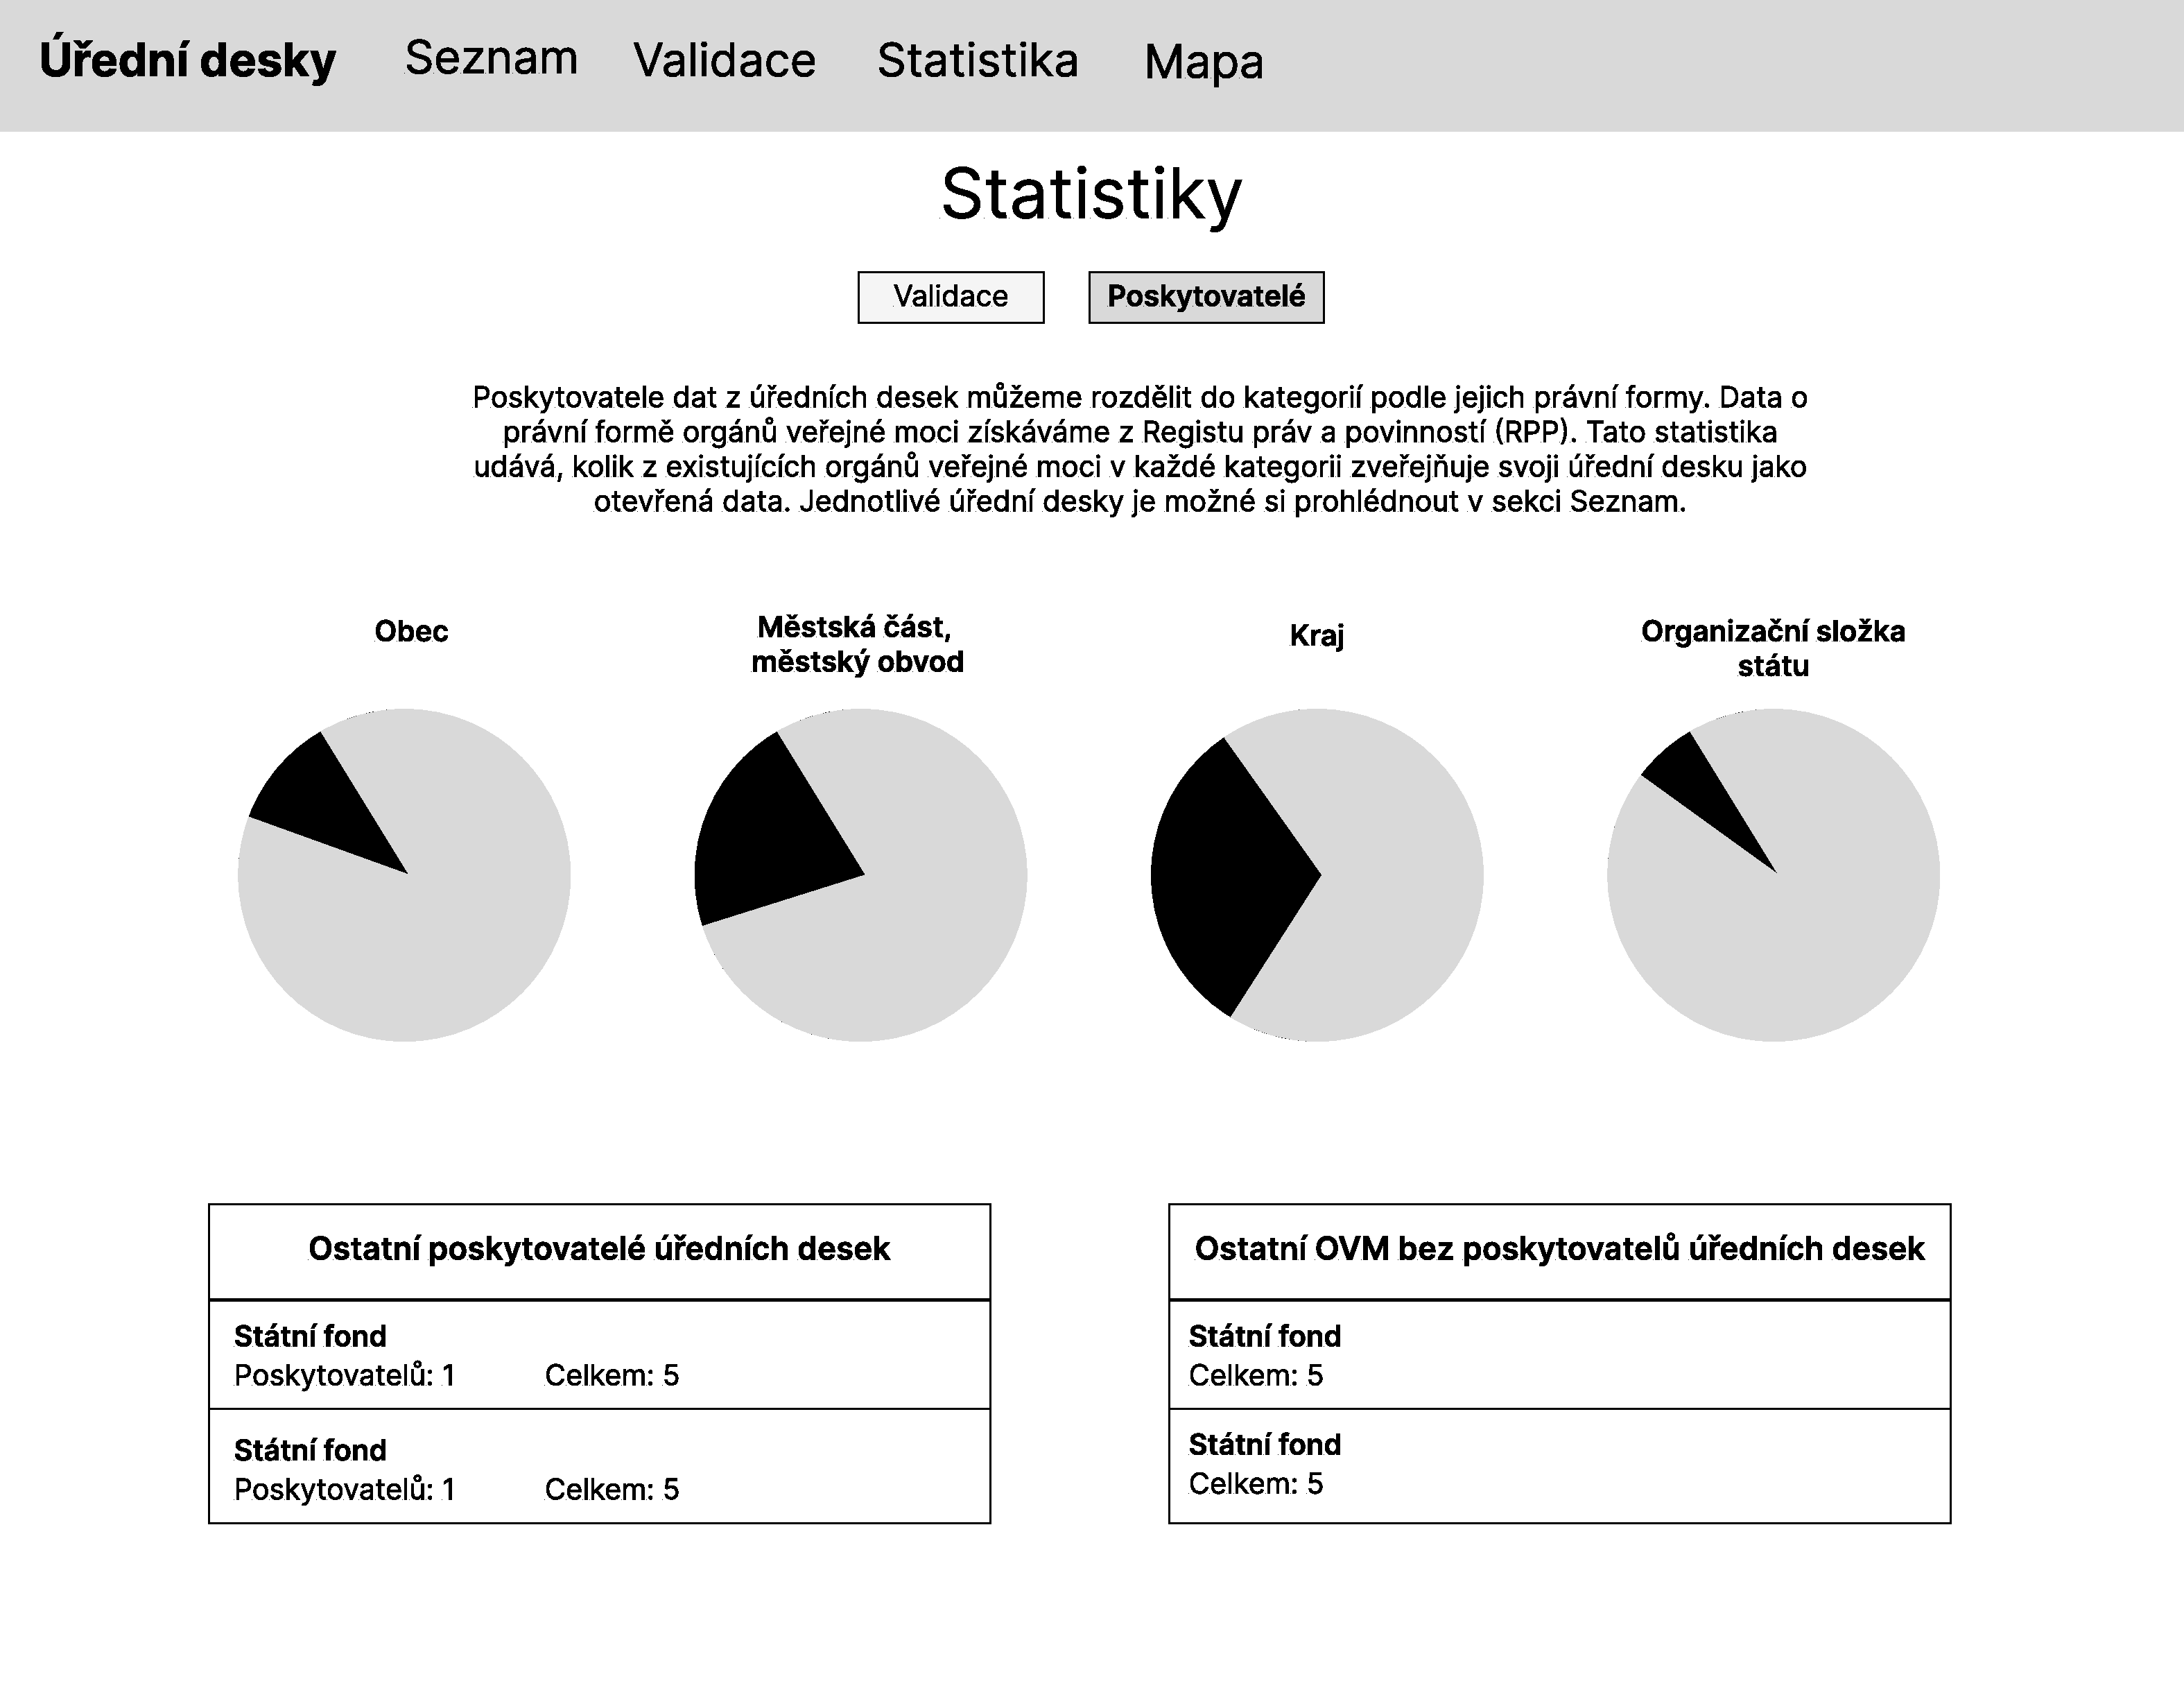
\includegraphics[width=\textwidth, frame]{cs/obrazky/wireframes/wireframe_statistika_poskytovatele.pdf}
\caption{Návrh uživatelského rozhraní - Statistika poskytovatelů}
\label{fig:stat-poskyt}
\end{figure}


\section{Architektura}\label{sec:architektura}

Aplikace je navržená jako \emph{single-page application} implementovaná na straně klienta. To znamená, že aplikace pracuje bez serveru pouze na straně klienta a obsah aplikace je dynamicky renderovaný na základě interakce s uživatelem.

Toto řešení jsme zvolili pro splnění požadavku \textbf{T01} (viz \autoref{sub:tech-poz}), podle kterého by mělo být nasazení aplikace zprostředkováno pomocí služby GitHub Pages \footnote{\url{https://docs.github.com/en/pages/getting-started-with-github-pages}}. Tato služba umožňuje beplatné hostování webových aplikací z repozitáře na GitHub\footnote{\url{https://github.com/}}. V rámci služby je možné hostovat pouze statický obsah, nebo obsah renderovaný na straně klienta.

Detaily sestavení a nasazení aplikace jsou popsané v kapitole Implementace (\autoref{kap:implementace}).


\begin{figure} 
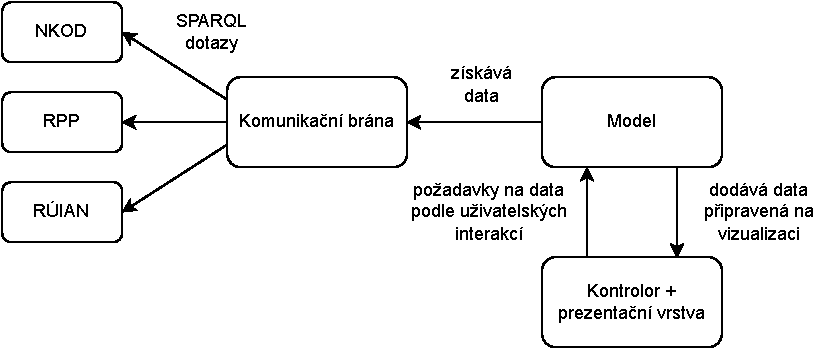
\includegraphics[width=\textwidth]{cs/obrazky/architektura_diagram.pdf}
\caption{Diagram architektury aplikace}
\label{fig:architektura}
\end{figure}

Diagram architektury najdeme na obrázku \ref{fig:architektura}.

Architekturu aplikace můžeme rozdělit na 3 části --- komunikační bránu, model a kontrolor s prezentační vrstvou.

\subsection{Komunikační brána}

První částí je komunikační brána. Tato část se stará o komunikaci s externími službami, jako jsou SPARQL endpointy NKOD, RPP a RÚIAN, a získávání dat, se kterými aplikace pracuje. Komunikační brána posílá dotazy na zmíněné endpointy a nad získanými daty provádí operace, kterými je konvertuje do podoby, ve které data využívá zbývající část aplikace. Fungování komunikační brány je podrobněji popsáno v části \ref{sec:ziskavani-dat}, Získávání dat.

\subsection{Model}

Druhou částí je model, který obsahuje abstrakce nad strukturami popsanými v OFN pro úřední desky. Nejdůležitějšími strukturami, se kterými model pracuje jsou:
\begin{itemize}
    \item struktura odpovídající datasetu v NKOD --- obsahuje název úřední desky, informace o poskytovateli atd.
    \item struktura odpovídající distribuci datasetu --- obsahuje položky podle OFN pro úřední desky
\end{itemize}

Model v sobě drží data, která používá prezentační vrstva aplikace a která nabízí jako následující abstrakce:
\begin{itemize}
    \item úřední deska --- obsahuje metadata podle OFN pro úřední desky a je možné z ní získat seznam informací, které jsou na ní vyvěšené.
    \item informace --- představuje jednu informaci vyvěšenou na úřední desce, obsahuje metadata podle OFN pro úřední desky
    \item dokument --- dokument, který je přílohou informace, obsahuje metadata podle OFN specifikace pro Digitální objekt \cite{OFN-Dig}
\end{itemize}

\subsection{Kontrolor a prezenční vrstva}

Třetí částí je kontrolor a prezenční vrstva. Prezenční vrstva vizualizuje data z modelu a vytváří uživatelské rozhraní. Kontrolor na základě podnětů z uživatelského rozhraní vyvolává změny v modelu, které se pak promítají do změn ve vizualizaci prezenční vrstvy. 

Interakce částí architektury může vypadat následovně. Uživatel v aplikačním rozhraní přejde do jiného modulu aplikace. Kontrolor zaznamená požadavek na nový modul a využije rozhraní modelu k požadavku na data, která se mají zobrazit v daném modulu. Model pošle požadavek na příslušnou část komunikační brány k získání dat. Komunikační brána zformuluje a pošle SPARQL dotaz na příslušný endpoint, data získaná z endpointu naparsuje a zpracuje do podoby, které rozumí model. Pak data předá modelu. Model nad získanými daty postaví abstrakce, které se využívají při vizualizaci. Prezentační vrstva získá data z modelu a vizualizuje.

\section{Získávání dat}\label{sec:ziskavani-dat}

V této sekci bude popsáno, jak aplikace získává data interakcí s externími systémy. Na obrázku \ref{fig:konc-model} můžeme vidět konceptuální model dat, se kterými aplikace pracuje. V modelu jsou barevně vyznačené zdroje, ze kterých data získáváme. V následujícím textu tyto zdroje postupně popíšeme.

\begin{figure} 
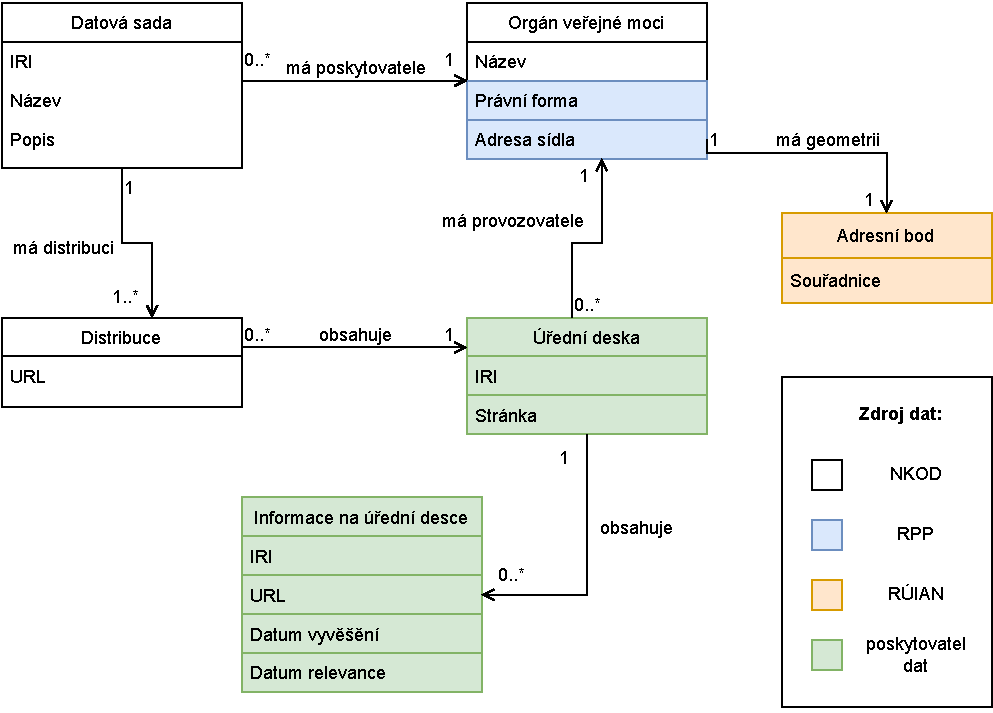
\includegraphics[width=\textwidth]{cs/obrazky/konceptualni_model.pdf}
\caption{Konceptuální model}
\label{fig:konc-model}
\end{figure}

Některé texty v ukázkách dat a některá URL byla pro potřeby práce zkrácena.

\subsection{Datové sady s úředními deskami}

Aplikace používá NKOD k nalezení datových sad s informacemi z úředních desek. Aplikace provádí SPARQL dotazy na endpoint NKOD \footnote{\url{https://data.gov.cz/sparql}}. Následuje příklad SPARQL dotazu (ukázka \ref{code:nkod-dotaz}), který získává z NKOD metadata k datovým sadám s úředními deskami. Dotaz je také možné zobrazit a spustit ve webové aplikaci \href{https://api.triplydb.com/s/aey-LUG7p}{Yasgui}.

%\inputminted{sql}{cs/kod/vsechny_desky.rq}
%\begin{minted}{sql}

\begin{figure}[h]
    \label{code:nkod-dotaz}
    \begin{code}

PREFIX foaf: <http://xmlns.com/foaf/0.1/>
PREFIX dcterms: <http://purl.org/dc/terms/>
PREFIX dcat: <http://www.w3.org/ns/dcat#>
PREFIX l-sgov-sbírka-111-2009-pojem:
<https://slovník.gov.cz/legislativní/sbírka/111/2009/pojem/>

SELECT  ?název ?popis ?poskytovatel ?poskytovatel_iri ?zdroj
WHERE {
    ?s a dcat:Dataset ;
        dcat:distribution ?distribuce ;
        dcterms:conformsTo 
            <https://ofn.gov.cz/úřední-desky/2021-07-20/> ;
        dcterms:title ?název ;
        dcterms:description ?popis;
        dcterms:publisher ?poskytovatel_iri .
    ?distribuce a dcat:Distribution ;
        dcterms:format
            <http://publications.europa.eu/.../file-type/JSON_LD> ;
        dcat:downloadURL ?zdroj .
  FILTER (langMatches(LANG(?název), "cs"))
  FILTER (langMatches(LANG(?popis), "cs"))
  OPTIONAL {
       ?poskytovatel_iri
       l-sgov-sbírka-111-2009-pojem:má-název-orgánu-veřejné-moci
           ?ovm_název_poskytovatele 
  }
  OPTIONAL {
       ?poskytovatel_iri foaf:name ?nkod_název_poskytovatele
  }
  BIND(COALESCE(?ovm_název_poskytovatele, ?nkod_název_poskytovatele)
    AS ?poskytovatel)

}
LIMIT 1
\end{code}
\caption{SPARQL dotaz na NKOD pro získání úředních desek}
\end{figure}

%\end{minted}

Dotaz získá všechny datové sady, které odpovídají specifikaci OFN pro úřední desky \url{https://ofn.gov.cz/úřední-desky/2021-07-20/} pomocí predikátu \\
\texttt{dcterms:conformsTo}. 
V rámci datové sady vybere distribuci ve formátu JSON-LD (predikát \texttt{dcterms:format}) a získá URL distribuce ke stažení (predikát \\ \texttt{dcterms:downloadURL}). 


\begin{figure}[h!]
    \label{code:nkod-res}
\begin{code}
{
  "head": {
    "link": [],
    "vars": [
      "název",
      "popis",
      "poskytovatel",
      "zdroj"
    ]
  },
  "results": {
    "distinct": false,
    "ordered": true,
    "bindings": [
      {
        "název": {
          "type": "literal",
          "xml:lang": "cs",
          "value": "Úřední deska MČ Praha 3"
        },
        "popis": {
          "type": "literal",
          "xml:lang": "cs",
          "value": "Tato datová sada obsahuje data ..."
        },
        "poskytovatel": {
          "type": "literal",
          "xml:lang": "cs",
          "value": "Městská část Praha 3"
        },
        "poskytovatel_iri": {
          "type": "uri",
          "value": 
            "https://rpp-opendata...cz/.../orgán-veřejné-moci/00063517"
        },
        "zdroj": {
          "type": "uri",
          "value": "https://www.praha3.cz/eDeska/opendata"
        }
      }
    ]
  }
}
\end{code}
\caption{Příklad odpovědi z NKOD}
\end{figure}

Z metadat datové sady také získá název (predikát \texttt{dcterms:title}) a popis datové sady (predikát \texttt{dcterms:description}) v českém jazyce a název poskytovatele. U poskytovatele rozlišuje, jestli se jedná o orgán veřejné moci. Pro potřeby práce je výstup omezen 1 výsledek.

Odpověď z NKOD aplikace dostane ve formátu JSON (ukázka \ref{code:nkod-res}). Odpověď obsahuje hlavičku s názvem datový položek, dále následují získaná metadata. Vidíme, že názvy klíčů v ukázce \ref{code:nkod-res} odpovídají názvům proměných ve SPARQL dotazu \ref{code:nkod-dotaz}.

Při zobrazování konkrétní úřední desky, aplikace použije URL distribuce ke stažení dat ze serveru poskytovatele.

IRI datové sady se v aplikaci využívá jako jednoznačný identifikátor úřední desky. Umístěním IRI jako parametru do URL v aplikaci je možné získat odkaz na vizualizaci konkrétní úřední desky. IRI se také používá pro vytvoření odkazu na datovou sadu na webu NKOD.

\subsection{Data z úředních desek}

Samotná data z úředních desek zveřejňuje poskytovatel na adrese, kterou dostaneme jako URL distribuce z dotazu na NKOD popsaného výše. Data pak získáme HTTP požadavkem na dané URL. Data z úředních desek jsou zveřejňovaná ve formátu JSON-LD \cite{JSON-LD} a odpovídají specifikaci OFN pro úřední desky \cite{OFN-UD}.

\begin{figure}[h]
    \label{code:rpp-dotaz}
\begin{code}
PREFIX a-sgov-104-pojem: <https://slovník.gov.cz/agendový/104/pojem/>
PREFIX l-sgov-sbírka-111-2009-pojem:
<https://slovník.gov.cz/legislativní/sbírka/111/2009/pojem/>
PREFIX skos: <http://www.w3.org/2004/02/skos/core#>

SELECT DISTINCT 
    ?nazev ?ico ?cisloPravniFormy ?nazevPravniFormy ?sidlo
WHERE {
  <https://rpp-opendata.egon.gov.cz/.../orgán-veřejné-moci/00063517> 
    a l-sgov-sbírka-111-2009-pojem:orgán-veřejné-moci ;
	l-sgov-sbírka-111-2009-pojem:
	    má-identifikační-číslo-osoby-orgánu-veřejné-moci 
	    ?ico ;
    l-sgov-sbírka-111-2009-pojem:má-právní-formu-osoby 
	    ?pravni_forma ;
  	l-sgov-sbírka-111-2009-pojem:má-název-orgánu-veřejné-moci 
  	    ?nazev ;
    l-sgov-sbírka-111-2009-pojem:má-adresu-sídla-orgánu-veřejné-moci 
        ?sidlo .
  
?pravni_forma   skos:notation ?cisloPravniFormy ;
                skos:prefLabel ?nazevPravniFormy .    
FILTER (LANG(?nazev) = 'cs') 
}
\end{code}
\caption{SPARQL dotaz na RPP - vlastnosti OVM}
\end{figure}

\subsection{Informace o poskytovateli}

V aplikaci je možné třídění úředních desek do kategorií na základě právní formy poskytovatele (obce, kraje, organizační složky státu atp.). 

Jak již bylo popsáno (viz \autoref{subsec:ofn-uredni}) rozlišujeme provozovatele úřední desky a poskytovatele dat v NKOD. Roztřídění úředních desek podle právní formy orgánu aplikace provádí na základě poskytovatele dat z NKOD, tedy ne přímo podle úřadu, který desku spravuje. Toto rozhodnutí můžeme zdůvodnit tím, že ve většině případů se jedná o zaštiťující nebo jinak propojenou organizaci, tedy její právní forma je shodná s právní formou vlastníka desky a je dosaženo stejného výsledku. 

Navíc, získání informace o provozovateli desky je možné pouze z distribuce, tedy pro roztřídění desek do kategorií by bylo nutné stáhnout distribuce všech desek. Toto řešení by se při počtu úředních desek v řádu stovek (a potenciálně tisíců) jevilo jako nevhodné, protože by zbytečně navyšovalo požadavky na připojení uživatele.

Při získávání úředních desek z NKOD v rámci metadat k datové sadě dostaneme název poskytovatele a jeho IRI (viz atributy \texttt{poskytovatel} a \\ \texttt{poskytovatel\_iri} v ukázce dat \ref{code:nkod-res}). IRI se odkazuje do RPP, kde je možné získat další informace o poskytovateli, včetně jeho právní formy a adresy sídla.

Aplikace pro získání těchto dat využívá SPARQL endpoint RPP \footnote{\url{https://rpp-opendata.egon.gov.cz/odrpp/sparql}}. Následuje příklad SPARQL dotazu (ukázka \ref{code:rpp-dotaz}, spustit dotaz v \href{https://api.triplydb.com/s/nPcS7GirV}{Yasgui}) na konkrétní orgán veřejné moci (Městskou část Praha 3) s použitím IRI orgánu, který získá IČO  orgánu (predikát \texttt{má-identifikační-číslo-osoby-orgánu-veřejné-moci}) a jeho právní formu (predikát \texttt{má-právní-formu-osoby}). Z IRI právní formy získá její název a číslo. 

Dotaz také získá adresu sídla orgánu (predikát \\ \texttt{má-adresu-sídla-orgánu-veřejné-moci}), která se využívá pro umístění poskytovatele na mapu.


Odpověď na dotaz z RPP ve formátu JSON je v ukázce \ref{code:rpp-res}. V datech vidíme, že se opravdu jedná o Městskou část Praha 3. Právní forma orgánu je 811, tedy \uv{Městská část, městský obvod}, což odpovídá.
V položce \texttt{sídlo} získáme adresu sídla v podobě IRI adresního místa v RÚIAN.

\begin{figure}
\begin{code}
{
  "head": {
    "link": [],
    "vars": [
      "nazev",
      "ico",
      "cisloPravniFormy",
      "nazevPravniFormy",
      "sidlo"
    ]
  },
  "results": {
    "distinct": false,
    "ordered": true,
    "bindings": [
      {
        "nazev": {
          "type": "literal",
          "xml:lang": "cs",
          "value": "Městská část Praha 3"
        },
        "ico": {
          "type": "typed-literal",
          "datatype": "http://www.w3.org/2001/XMLSchema#string",
          "value": "00063517"
        },
        "cisloPravniFormy": {
          "type": "typed-literal",
          "datatype": "http://www.w3.org/2001/XMLSchema#string",
          "value": "811"
        },
        "nazevPravniFormy": {
          "type": "literal",
          "xml:lang": "cs",
          "value": "Městská část, městský obvod"
        },
        "sidlo": {
          "type": "uri",
          "value": "https://linked.cuzk.cz/.../adresni-misto/21773998"
        }
      }
    ]
  }
}
\end{code}
\caption{Příklad odpovědi z RPP}
\label{code:rpp-res}
\end{figure}

\subsection{Souřadnice adresy sídla}

V aplikaci vizualizujeme úřední desky také na mapě, kam je umístíme podle adresy poskytovatele. Adresu získáme jako IRI adresního místa v RÚIAN. Aby\-chom mohli adresu zobrazit na mapě, potřebujeme z IRI adresního bodu získat souřadnice.

V ukázce \ref{code:ruian-dotaz} můžeme vidět SPARQL dotaz na endpoint RÚI\-AN \footnote{\url{https://linked.cuzk.cz.opendata.cz/sparql}} (spustit dotaz v \href{https://api.triplydb.com/s/7jxqEz6LL}{Yasgui}), který ukazuje, jak získat souřadnice bodu z adresního místa, které získáme jako sídlo orgánu veřejné moci z RPP.

\begin{figure}
    \label{code:ruian-dotaz}
\begin{code}
PREFIX schema: <http://schema.org/>     
PREFIX locn: <http://www.w3.org/ns/locn#>     
SELECT DISTINCT ?geometrie     
WHERE {      
    ?iri    a schema:Place ;          
            locn:geometry ?geometrie .       
VALUES ?iri {
<https://linked.cuzk.cz/resource/ruian/adresni-misto/21773998> 
    } 
}
\end{code}
\caption{SPARQL dotaz na RÚIAN - souřadnice adresního bodu}
\end{figure}


V dotazu používáme klazuli \texttt{VALUES}, do proměnné \texttt{iri} přiřadíme všechna IRI adresních míst, pro která chceme získat souřadnice. V našem příkladu se jedná pouze o jednu adresu (sídlo úřadu městské části Praha 3), v dotazu v aplikaci do klauzule napíšeme IRI adres všech poskytovatelů, u kterých chceme znát souřadnice.

Souřadnice adresního bodu v odpovědi (ukázka \ref{code:ruian-res}) získáme ve formátu Well-Known Text \cite{WKT} --- \texttt{POINT(14.454011740852664 50.08474823342625)}.

\begin{figure}[h]
    \label{code:ruian-res}
\begin{code}
{
  "head": {
    "link": [],
    "vars": [
      "geometrie"
    ]
  },
  "results": {
    "distinct": false,
    "ordered": true,
    "bindings": [
      {
        "geometrie": {
          "type": "typed-literal",
          "datatype": "http://www.opengis.net/ont/gml#wktLiteral",
          "value": "POINT(14.454011740852664 50.08474823342625)"
        }
      }
    ]
  }
}
\end{code}
\caption{Příklad odpovědi z RÚIAN}
\end{figure}


\chapter{Implementace}\label{kap:implementace}

V této kapitole bude popsána implementace aplikace, která byla provedena na základě návrhu aplikace v kapitole \ref{kap:navrh}. Aplikace je nasazená na adrese \url{https://bliakher.github.io/uredni_desky/}. Zdrojový kód aplikace je zveřejněný na platformě GitHub \footnote{\url{https://github.com/}} na URL \url{https://github.com/bliakher/uredni_desky} a jako příloha \ref{sub:repo1} v podobě snaphotu repozitáře ve formátu ZIP.

Kapitola se bude věnovat hlavně použitým technologiím a dalším implementačním rozhodnutím. Popis projektu včetně souborové struktury a jednotlivých tříd a rozhraní je možné najít ve vývojářské dokumentaci (\autoref{sec:developer-docs}).

\section{Použité technologie}

Jak bylo popsáno v návrhu, aplikace je implementovaná jako \textit{single-page application} na straně klienta. Pro implementaci byl použit programovací jazyk TypeScript v kombinaci s frameworkem React.

\subsection{TypeScript}

TypeScript \cite{TS} je silně typovaný programovací jazyk, který je nadstavbou jazyka JavaScript. TypeScript oproti jazyku JavaScript přidává možnost definovat typy a rozhraní a anotovat proměnné, parametry a návratové hodnoty metod, což umožňuje typovou kontrolu za kompilace. TypeScript je možné transpilovat do jazyka JavaScript, čímž se zajistí podpora na různých prohlížečích.

TypeScript byl pro implementaci projektu vybrán hlavně kvůli možnosti typování, čímž se snažíme vyhnout typovým chybám, které vznikají v jazyce JavaScript. Definovaní rozhraní jednotlivých částí aplikace navíc umožňuje lepší dokumentaci toku dat v aplikaci.

Aplikace využívá TypeScript verze 4.5.5 \footnote{\url{https://www.typescriptlang.org/docs/handbook/release-notes/typescript-4-5.html}}, který se transpiluje do ECMAScript verze 5 \cite{ecma5}

\subsection{React}

React\footnote{\url{https://reactjs.org/}} je deklarativní framework pro vývoj uživatelských rozhraní. Na základě studie od JetBrains \cite{JBStudie} se jedná o nejoblíbenější javascriptový framework pro vývoj uživatelských rozhraní. 

React využívá virtuální DOM s memoizací. V paměti si vytváří cache datových struktur, které tvoří aktuálně vyrenderovaný DOM, při aktualizaci vypočítá rozdíl nového a starého stavu a aktualizuje pouze ty části DOM stromu, které jsou ovlivněné změnou stavu. Selektivní renderování umožňuje větší výkon aplikace. \cite{ReactReconciliation}

React vytváří uživatelské rozhraní pomocí komponent. Komponenty jsou nezávislé jednotky, které si udržují vnitřní stav.\cite{ReactComponents} Na základě stavu se komponenta vyrenderuje podle příslušné šablony. Pro psaní šablon React využívá syntaxi JavaScript XML neboli JSX \cite{ReactJSX}, která umožňuje vytvářet HTML prvky v jazyce JavaScript. Díky tomu, mohou být šablony umístěné přímo v kódu.

Aplikace používá React ve verzi 17.0.2 \cite{Reactv17}.

\subsection{React Bootstrap}

Při implementaci byla také použitá knihovna React Bootstrap\footnote{\url{https://react-bootstrap.github.io/}} ve verzi 2.2.2, která obsahuje připravené React komponenty, sloužící pro ostylování aplikace. Jedná se hlavně o prvky pro pozicování, umožňující jednoduše vytvářet rozhraní, která se umí přizpůsobit různým velikostem displeje, a také ostylované řídící prvky, jako jsou tlačítka a formuláře.

Tato knihovna také nabízí velkou kolekci volně použitelných ikon, které je možné importovat jako komponenty.\footnote{\url{https://react-icons.github.io/react-icons}}

\section{Vývojové prostředí}

Vývoj probíhal v editoru Visual Studio Code \footnote{\url{https://code.visualstudio.com/}} s použitím rozšíření pro zvýraznění syntaxe jazyka TypeScript.

Pro instalaci a spravování knihoven byl použit správce balíčků npm \footnote{\url{https://www.npmjs.com/}} ve verzi 8.3.2. Sloužil také pro sestavení a spouštění aplikace pomocí šablony prostředí Create React App.

\subsection{Create React App}\label{sub:create-react}

Create React App\footnote{\url{https://www.npmjs.com/package/create-react-app}} je prostředí pro vývoj a sestavování aplikací v Reactu. Umí vygenerovat šablonu projektu, která podporuje TypeScript. Během vývoje aplikace je možné používat vývojový server, kdy se aplikace automaticky kompiluje a sestavuje po každé změně v kódu a spouští se v běhovém prostředí Node.js \footnote{\url{https://nodejs.org/en/about/}}.

Prostředí využívá kompilátor Babel \footnote{\url{https://babeljs.io/}} pro transpilaci TypeScriptu a JSX do JavaScriptu a Webpack \footnote{\url{https://webpack.js.org/}} pro zabalení kódu do balíčků se statickým obsahem.

Pro použití šablony Create React App je potřeba npm verze 5.6 nebo vyšší a Node.js verze 14 nebo vyšší.

\section{Verzování}

Při vývoji aplikace bylo použito verzování na platformě GitHub \footnote{\url{https://github.com/}}. Repozitář se zdrojovým kódem je dostupný na URL \\ \url{https://github.com/bliakher/uredni_desky} a jako příloha \ref{sub:repo1}. Stav repozitáře na moment odevzdání práce je označený tagem \texttt{odevzdani}.

GitHub je platforma podporující vývoj softwaru za pomoci verzovacího nástroje Git\footnote{\url{https://git-scm.com/}}, což je otevřený verzovací systém.

\section{Nasazení aplikace}

Aplikace je hostovaná pomocí služby GitHub Pages \footnote{\url{https://docs.github.com/en/pages/getting-started-with-github-pages/about-github-pages}} na adrese \url{https://bliakher.github.io/uredni_desky/}. V repozitáři na GitHub je nastavená větev projektu \textit{gh-pages}, ze které služba GitHub Pages bere obsah pro webovou aplikaci. Při aktualizaci větve se automaticky spustí proces, který nasadí novou verzi aplikace.

Pro sestavení aplikace pro nasazení je použit npm balíček gh-pages \footnote{\url{https://www.npmjs.com/package/gh-pages}}. Tento balíček vyrobí produkční build aplikace, který odešle do větve \textit{gh-pages}, což spustí publikaci na GitHub Pages.




\chapter{Dokumentace}\label{kap:dokumentace}

Tato kapitola je věnovaná dokumentaci, konkrétně uživatelské (\autoref{sec:user-docs}), vývojářské (\autoref{sec:developer-docs}) a administrátorské (\autoref{sec:admin-docs}). Dokumentace je také dostupná online na \url{https://bliakher.github.io/uredni_desky_docs/} a jako příloha \ref{sub:repo2}.

\section{Uživatelská dokumentace}\label{sec:user-docs}


V navigačním panelu aplikace najdeme odkazy do 4 částí aplikace: 
\begin{itemize}
    \item Seznam \autoref{seznam}
    \item Mapa \autoref{mapa}
    \item Statistiky \autoref{statistiky}
    \item Validace \autoref{validace}
\end{itemize}

\subsection*{Seznam}\label{seznam}

\begin{figure}
\centering
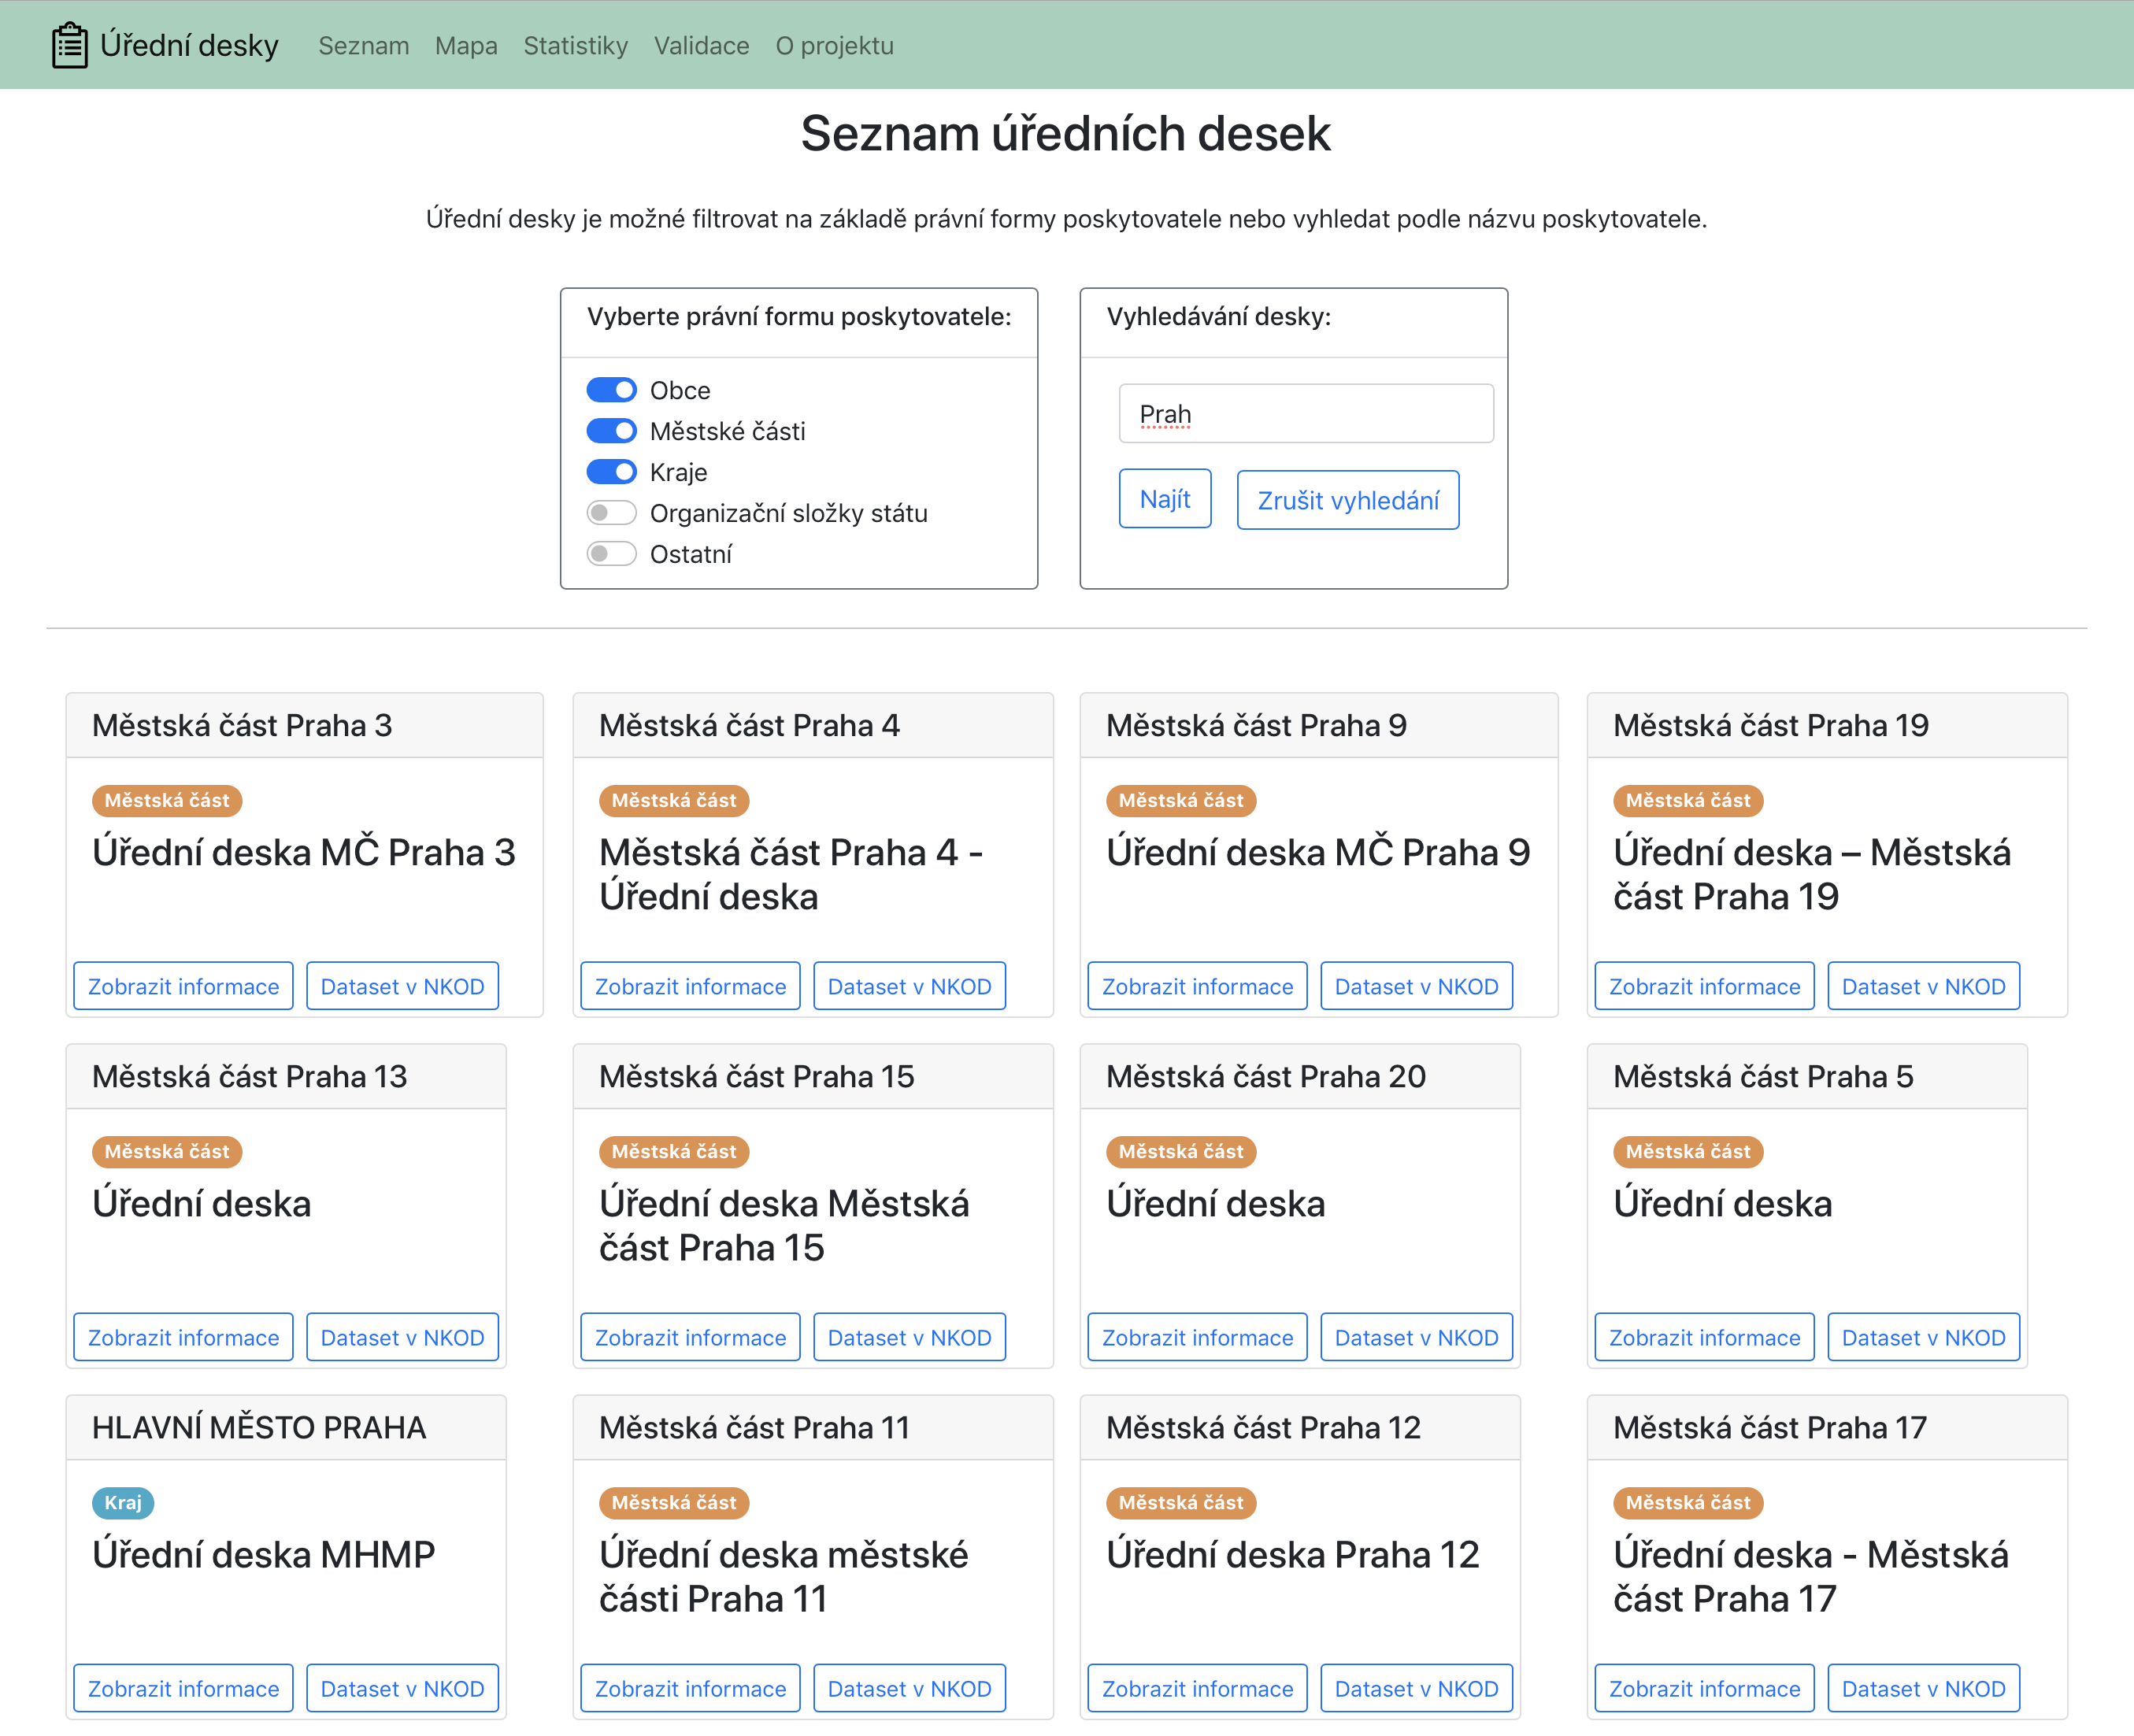
\includegraphics[width=\textwidth]{cs/obrazky/screenshots/seznam.png}
\caption{Ukázka filtrování v seznamu úředních desek}
\label{fig:screen-seznam}
\end{figure}

Tato část obsahuje seznam všech úředních desek, které má aplikace k
dispozici. Aplikace data z úředních desek získává z Národního katalogu
otevřených dat (NKOD), může tedy zobrazit pouze ty desky, které jsou
daným úřadem zveřejněné v NKOD jako otevřená data.

Úřední desky je možné filtrovat podle právní formy poskytovatele. Právní
formy, které podporujeme jsou: 
\begin{itemize}
    \item obce
    \item městské části a městské obvody
    \item kraje
    \item organizační složky státu
\end{itemize}

Právní formy poskytovatelů zjišťujeme z údajů uvedených v
\href{https://www.szrcr.cz/cs/registr-prav-a-povinnosti}{Registru práv a
povinností}. Poskytovatelé ostatních právních forem, nebo poskytovatelé,
u kterých nelze zjistit formu jsou v kategorii ostatní.

Pro filtrování desek použijte panel
\textit{Vyberte\ právní\ formu\ poskytovatele}. Nechte vybrané pouze ty
právní formy, jejichž poskytovatele chcete vyfiltrovat.

V úředních deskách je také možné vyhledávat na základě názvu desky nebo
jména poskytovatele pomocí formuláře pro vyhledávání.

Na obrázku \ref{fig:screen-seznam} je příklad seznamu, kde jsou vyfiltrované pouze úřední desky týkající se
Prahy od poskytovatelů s právními formami obec, městská část nebo kraj.

Ze seznamu je možné přejít na detail úřední desky zmáčknutím tlačítka \\
\textit{Zobrazit\ informace}. V detailu desky se zobrazují informace z
dané úřední desky, ve kterých je možné vyhledávat podle názvu s použitím
formuláře na vyhledávání.

\begin{figure}
\centering
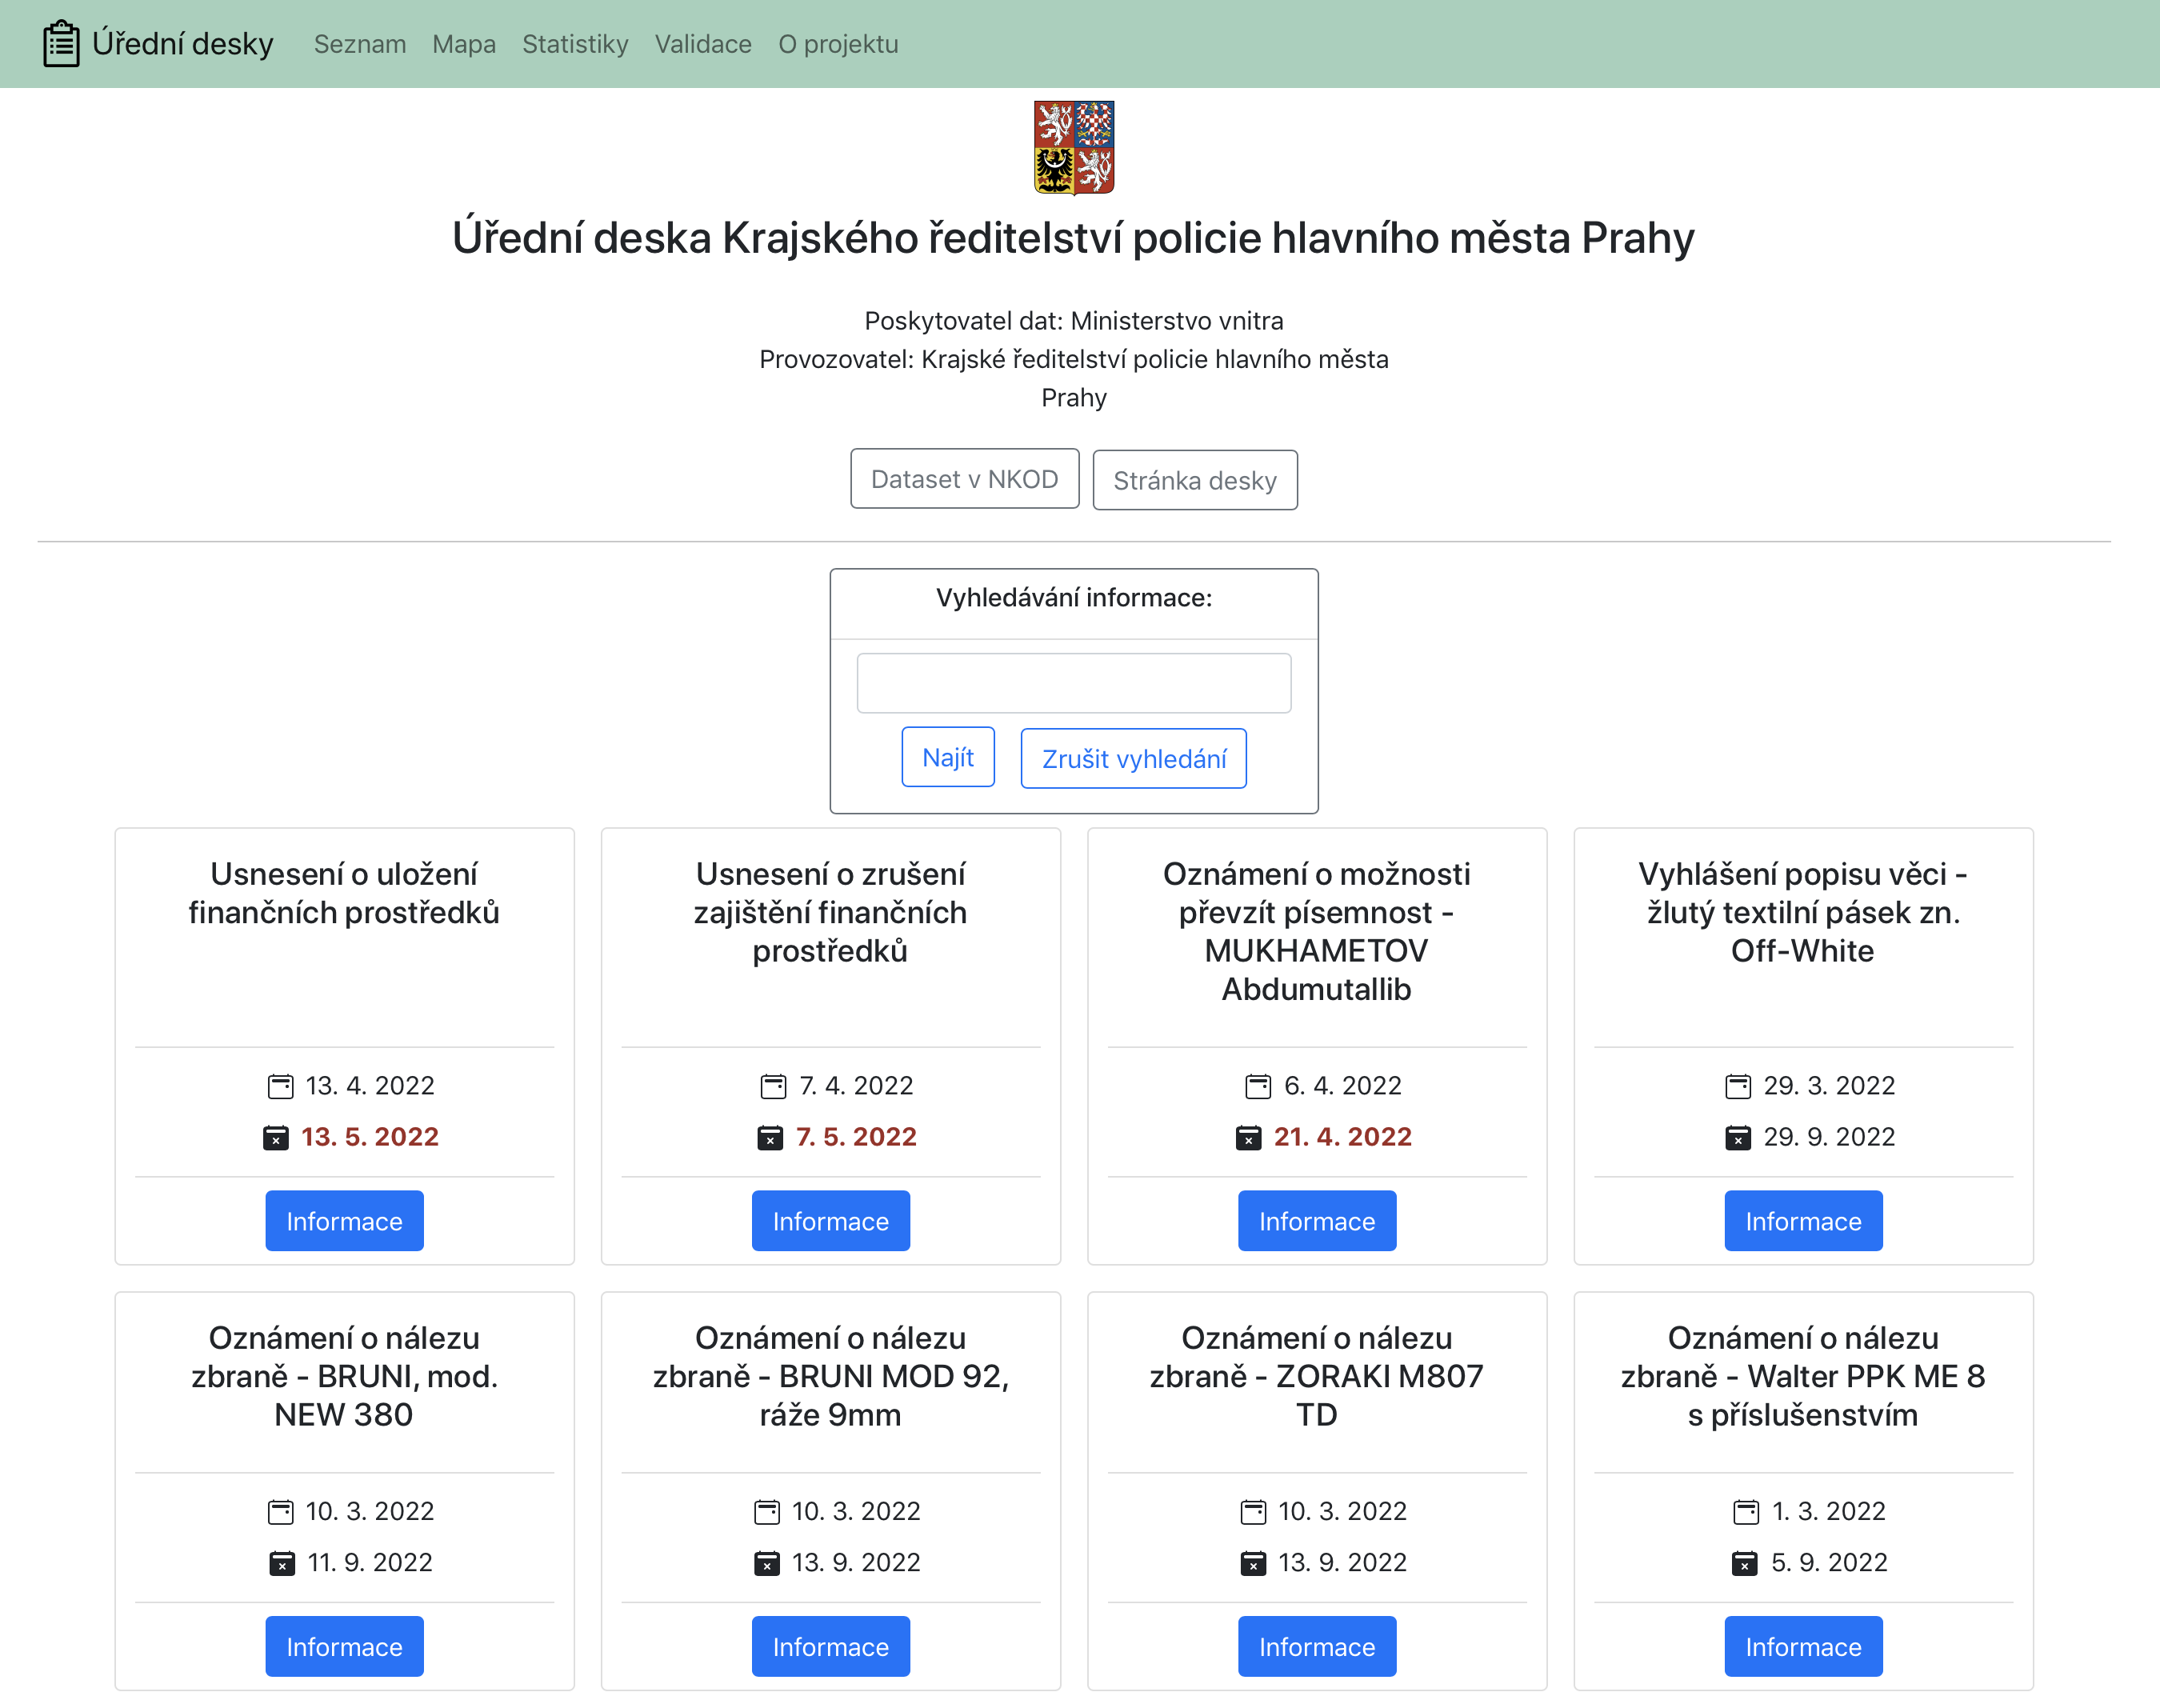
\includegraphics[width=\textwidth]{cs/obrazky/screenshots/detail.png}
\caption{Ukázka detailu úřední desky}
\label{fig:screen-detail}
\end{figure}

Na obrázku \ref{fig:screen-detail} vidíme příklad detailu úřední desky Krajského ředitelství policie
hl. m. Prahy. Pokud informace na desce již není relevantní, tedy datum relevance již
uplynulo, je datum zvýrazněné červeně.

\subsection*{Mapa}\label{mapa}

V této části jsou úřední desky zobrazené na mapě ČR. Úřední desky jsou
rozdělené podle poskytovatelů, kteří zveřejnili data v NKOD.
Poskytovatel je na mapě označen bodem, který je zbarvený podle právní
formy poskytovatele. Legenda k barvám je umístěná nad mapou.

Při kliknutí na bod na mapě se pod mapou zobrazí název daného
poskytovatele a všechny jeho úřední desky. Ze seznamu desek je opět
možné přejít do detailu desky.

Příklad zobrazení desky úřadu městské části Praha 13 z mapy je na obrázku \ref{fig:screen-mapa}.

\begin{figure}
\centering
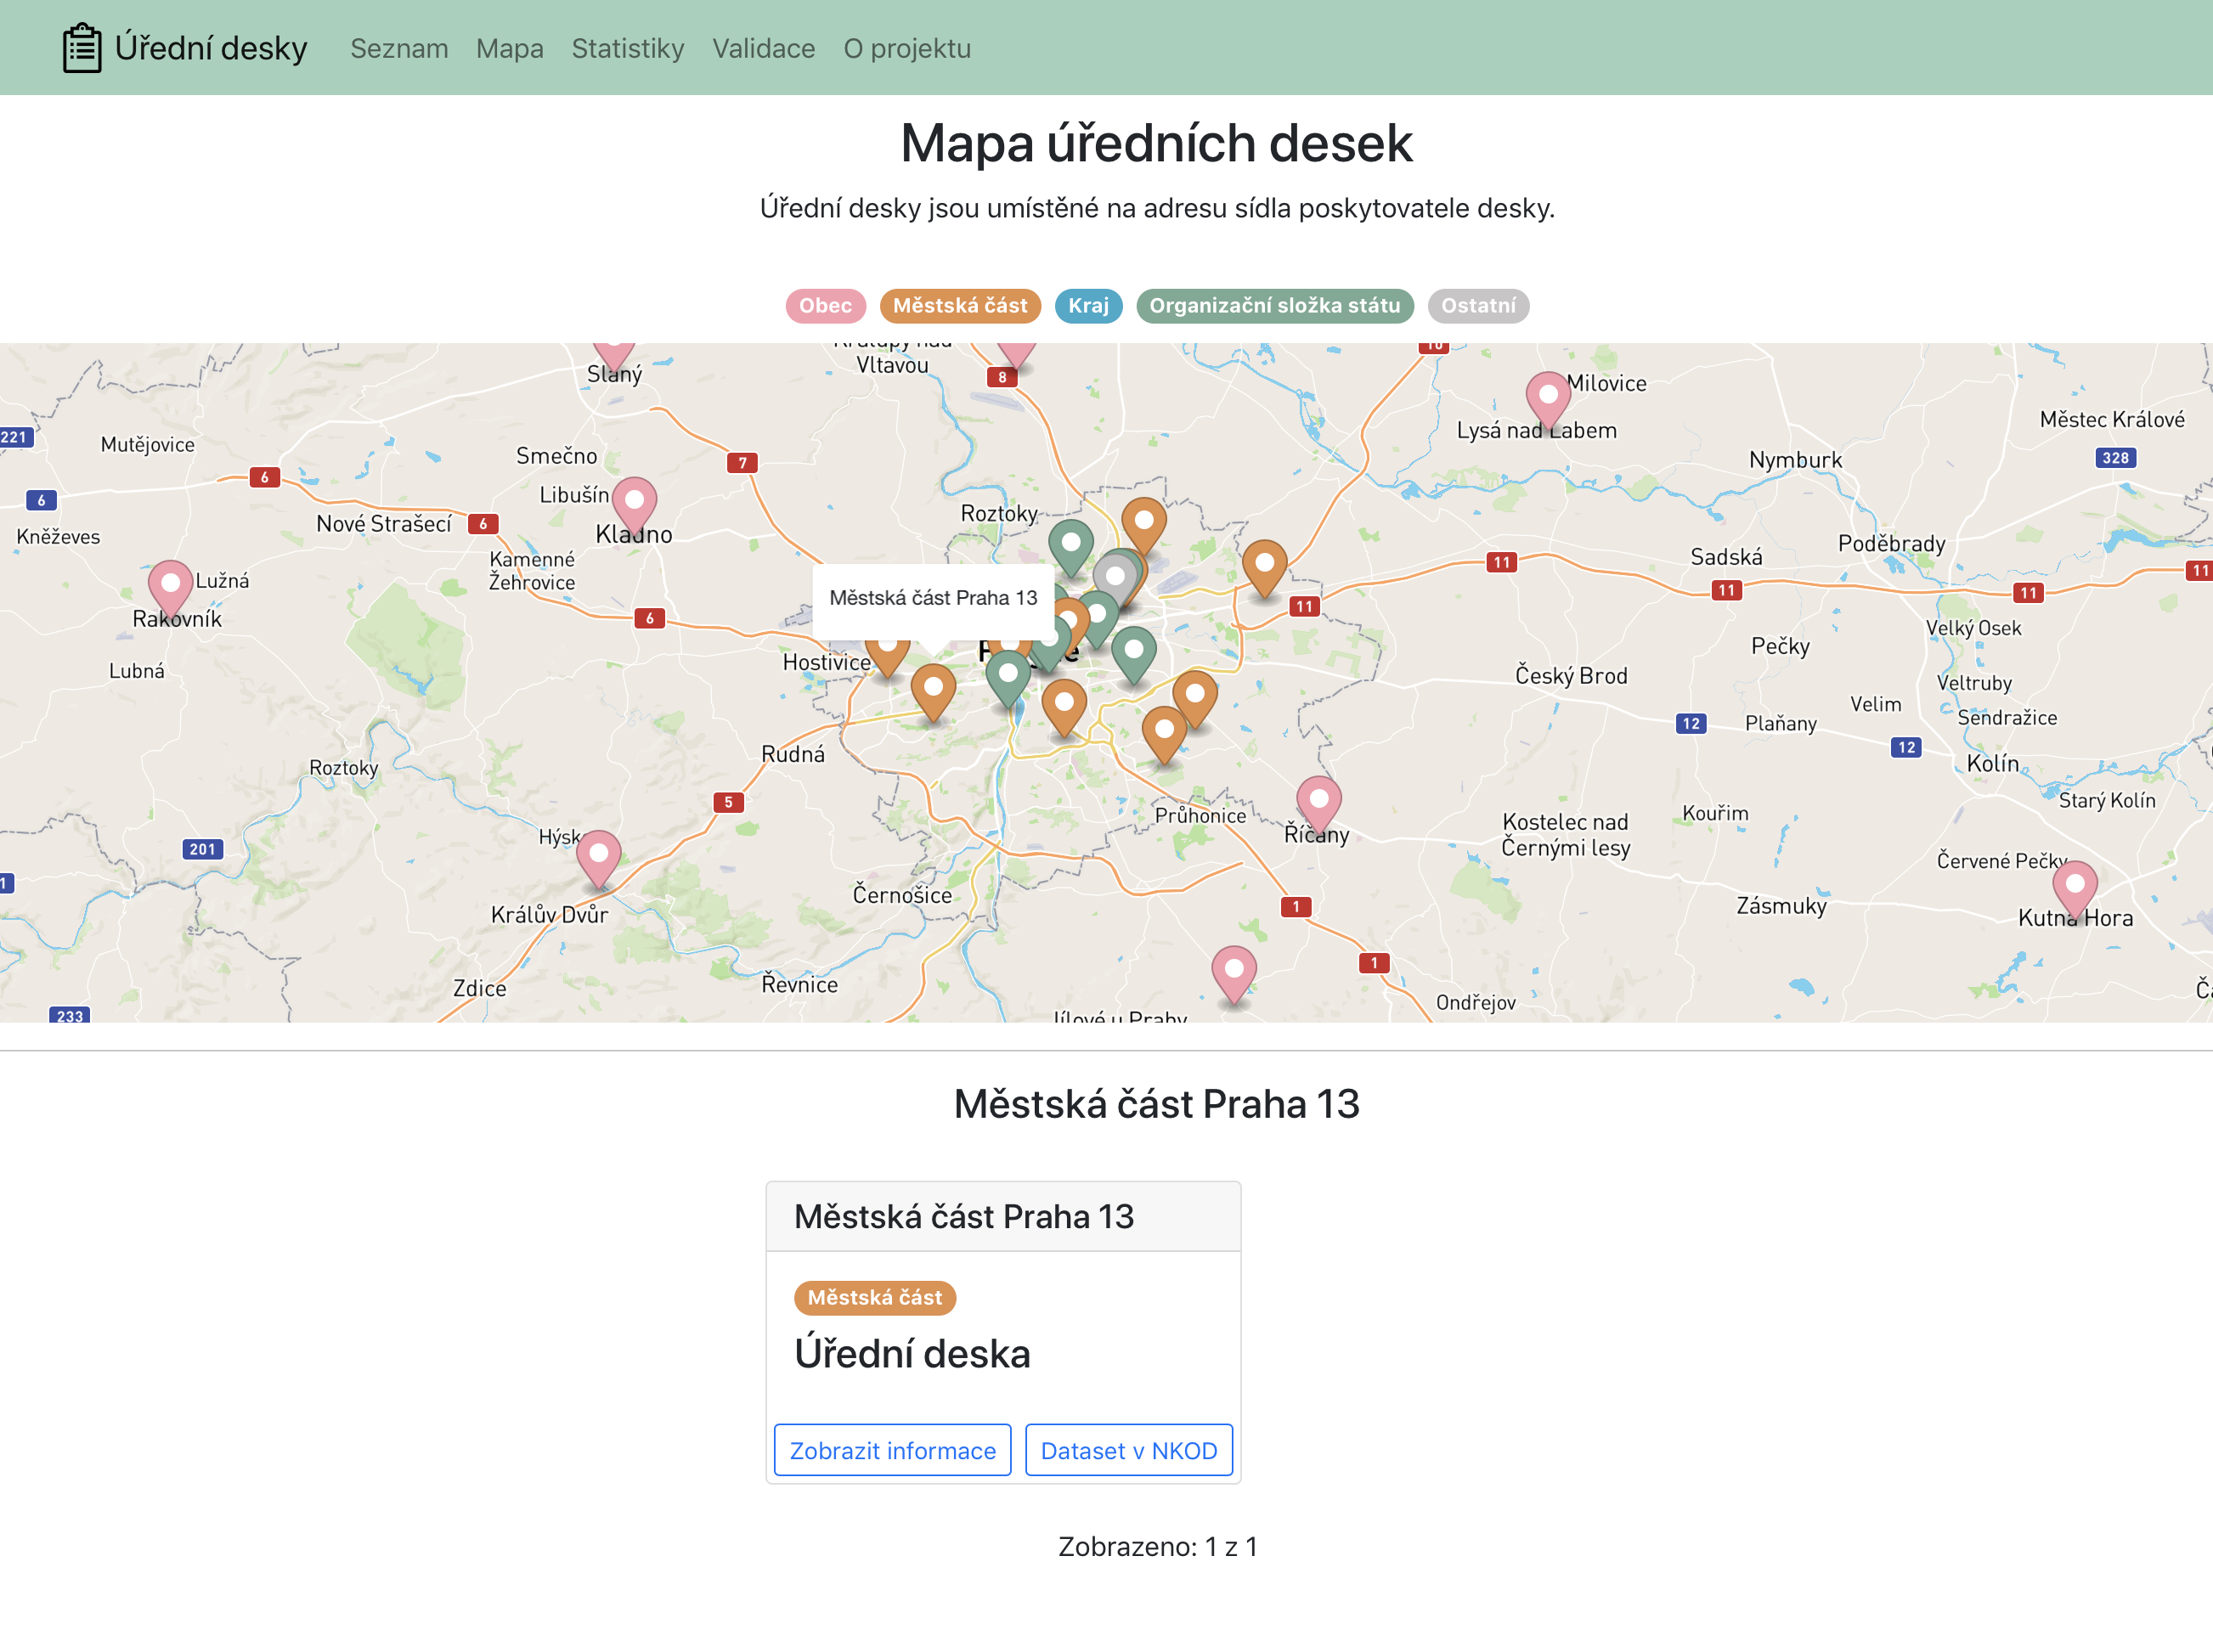
\includegraphics[width=\textwidth]{cs/obrazky/screenshots/mapa.png}
\caption{Ukázka zobrazení desky úřadu městské části Praha 13 na mapě}
\label{fig:screen-mapa}
\end{figure}

\subsection*{Validace}\label{validace}

Část validace je určená hlavně poskytovatelům dat. Provádí se zde
validace dat, konkrétně se kontroluje, jestli je data možné stáhnout a
jestli obsahují všechny doporučené parametry podle specifikace datového
formátu, podle kterého se mají zveřejňovat, který je určený
\href{https://ofn.gov.cz/úřední-desky/2021-07-20/}{Otevřenou formální
normou pro úřední desky}.

Výsledky validace jsou znázorněné tabulkou. Každý řádek tabulky
představuje shrnutí výsledků validace jedné úřední desky. Řádek obsahuje
název desky a jejího poskytovatele, informaci o tom, jestli je možné
stáhnout distribuci s daty desky, jestli data obsahují všechny
doporučené atributy a počet informací na desce.

Na obrázku \ref{fig:screen-validace} je příklad tabulky s výsledky validace, kde jsou vyfiltrované pouze
úřední desky městských částí. Pro větší přehlednost jsou řádky s deskou,
kde není možné stáhnout distribuci, obarvené červeně, a řádky desek, kde
chybí některé doporučené atributy, jsou obarvené žlutě.

\begin{figure}
\centering
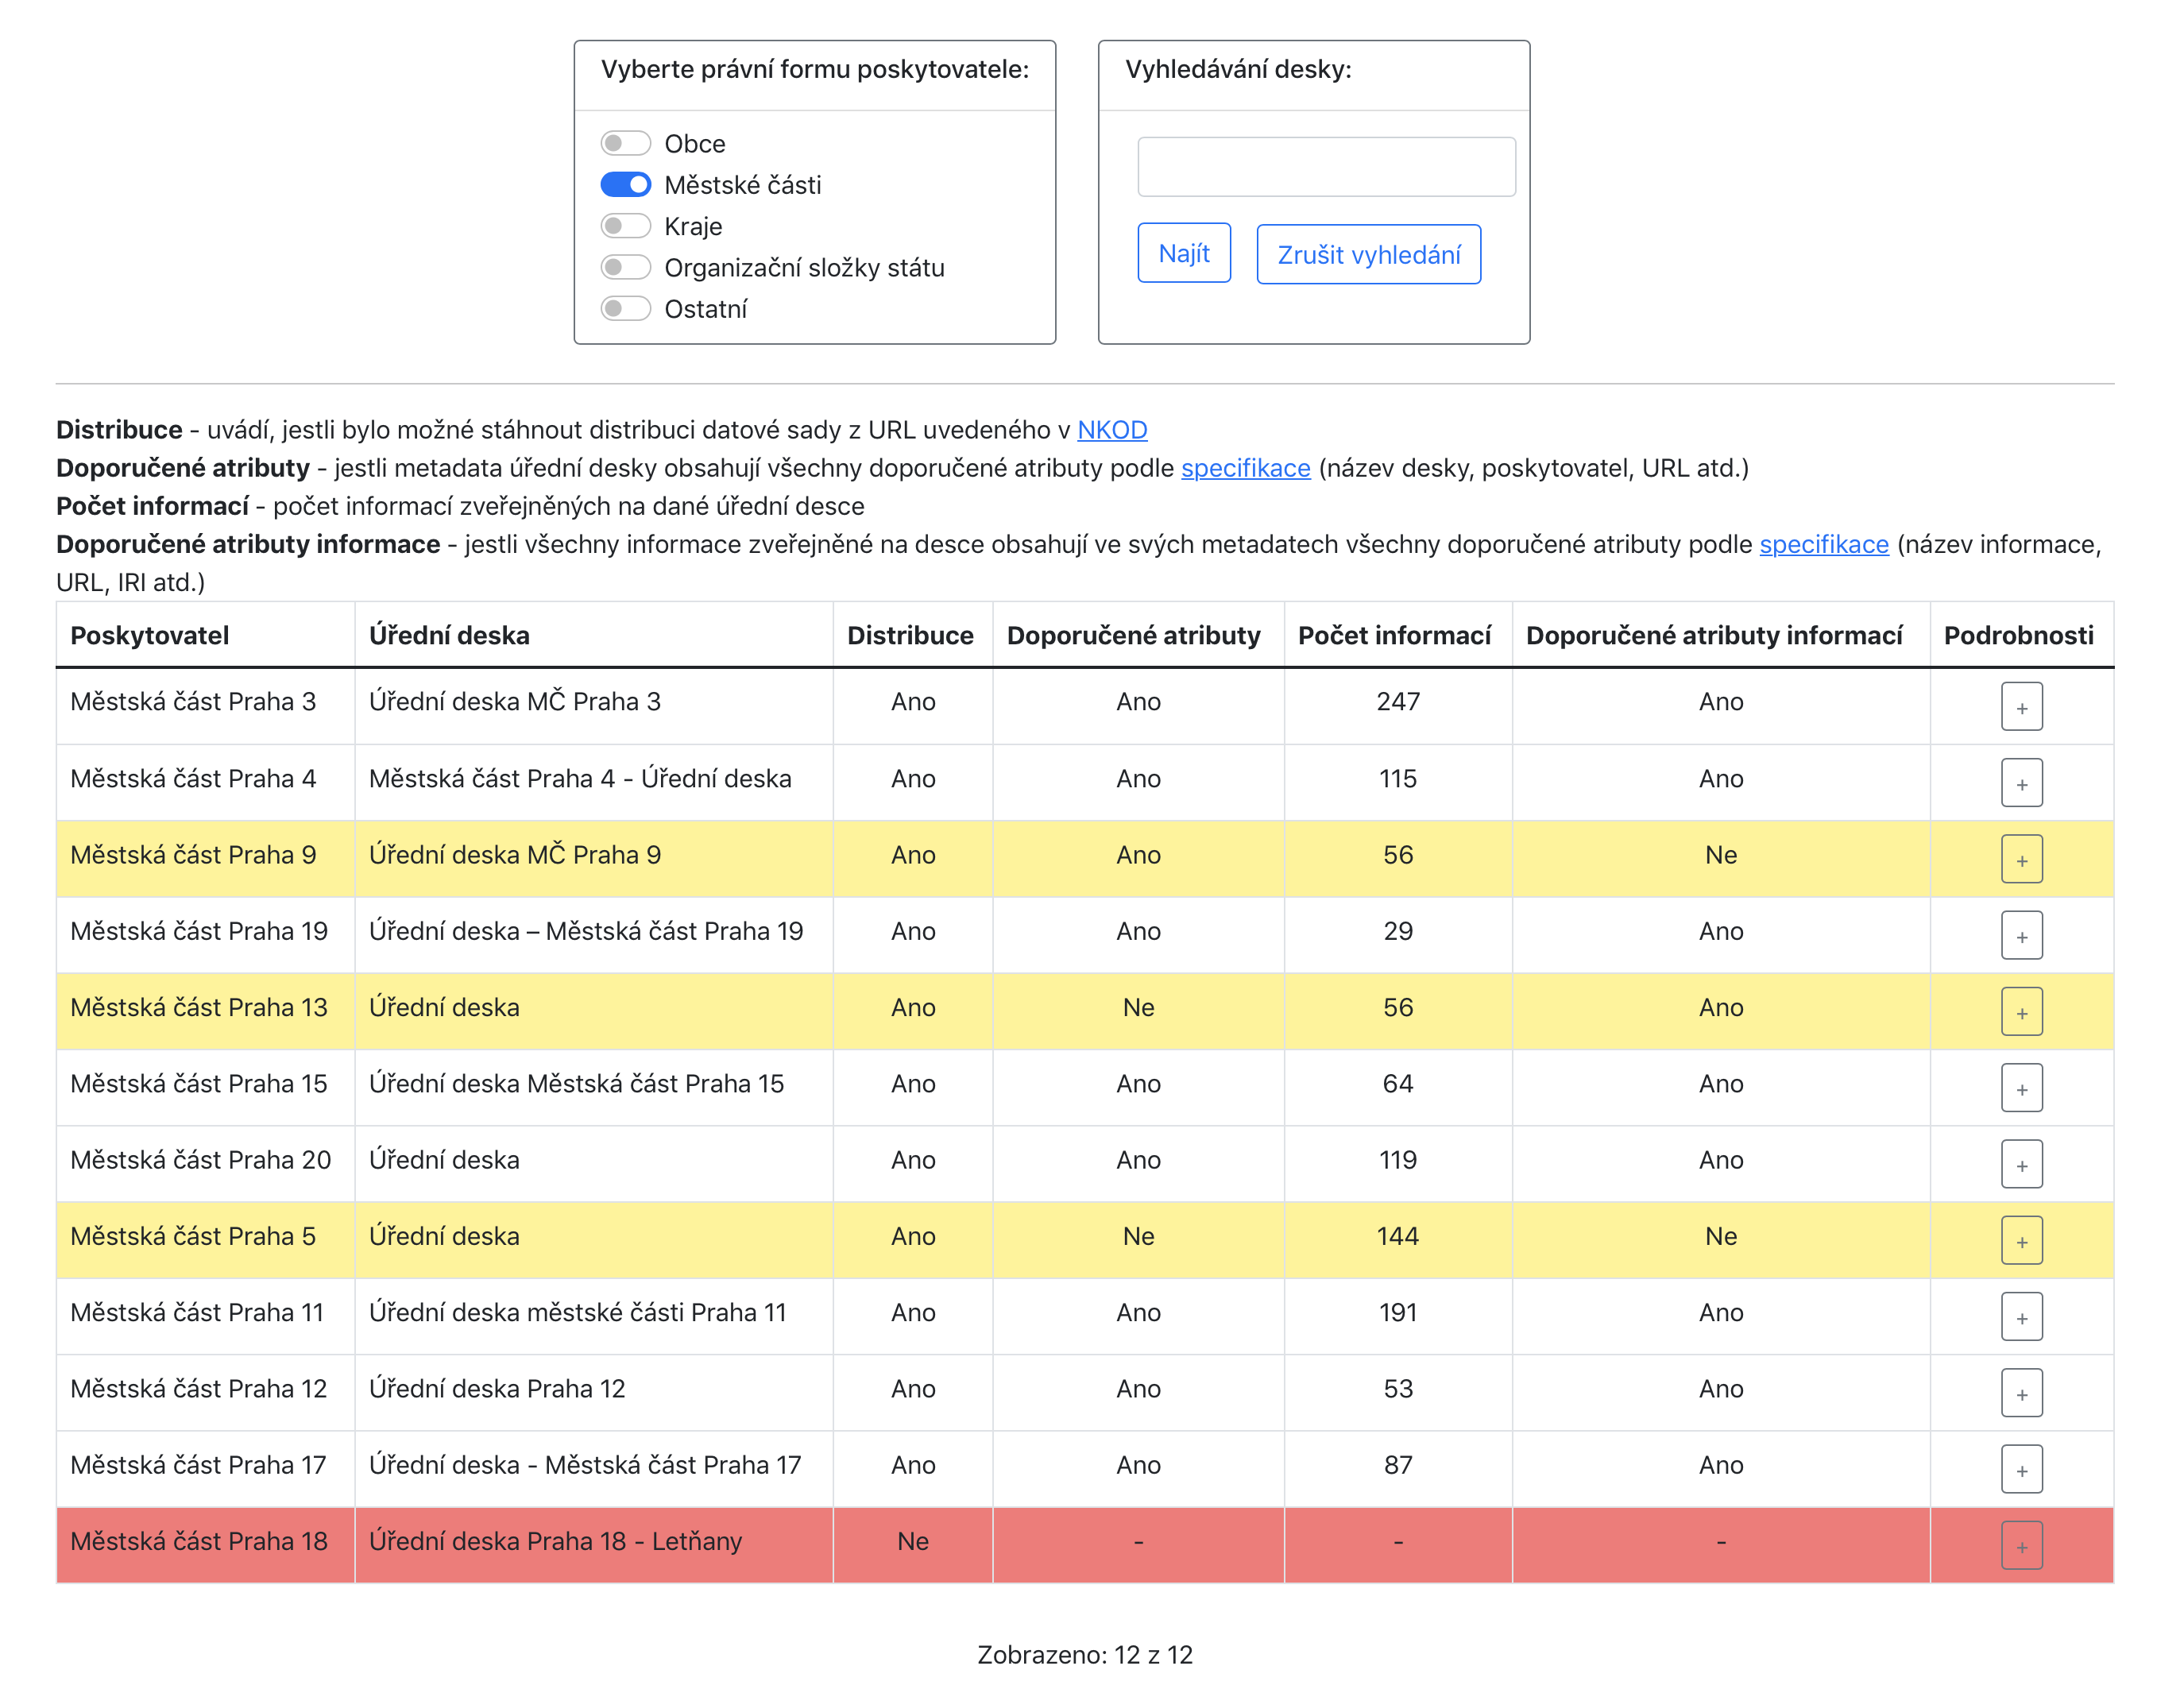
\includegraphics[width=\textwidth]{cs/obrazky/screenshots/validace.png}
\caption{Ukázka validace úředních desek poskytovatelů s právní formou městská část}
\label{fig:screen-validace}
\end{figure}

Z tabulky je možné se prokliknout na detail validace. Je zde vysvětleno,
jakým způsobem se validuje a jaký je význam jednotlivých doporučených
atributů (v části \textit{Jak\ validujeme?}).

Pokud distribuci desky není možné stáhnout, zobrazí se v detailu chybová
hláška získaná při stahování a seznam nejčastějších příčin, které tento
problém způsobují s odkazy na další informace o problému jako vidíme na
další ukázce, \autoref{fig:screen-validace-c}.

\begin{figure}
\centering
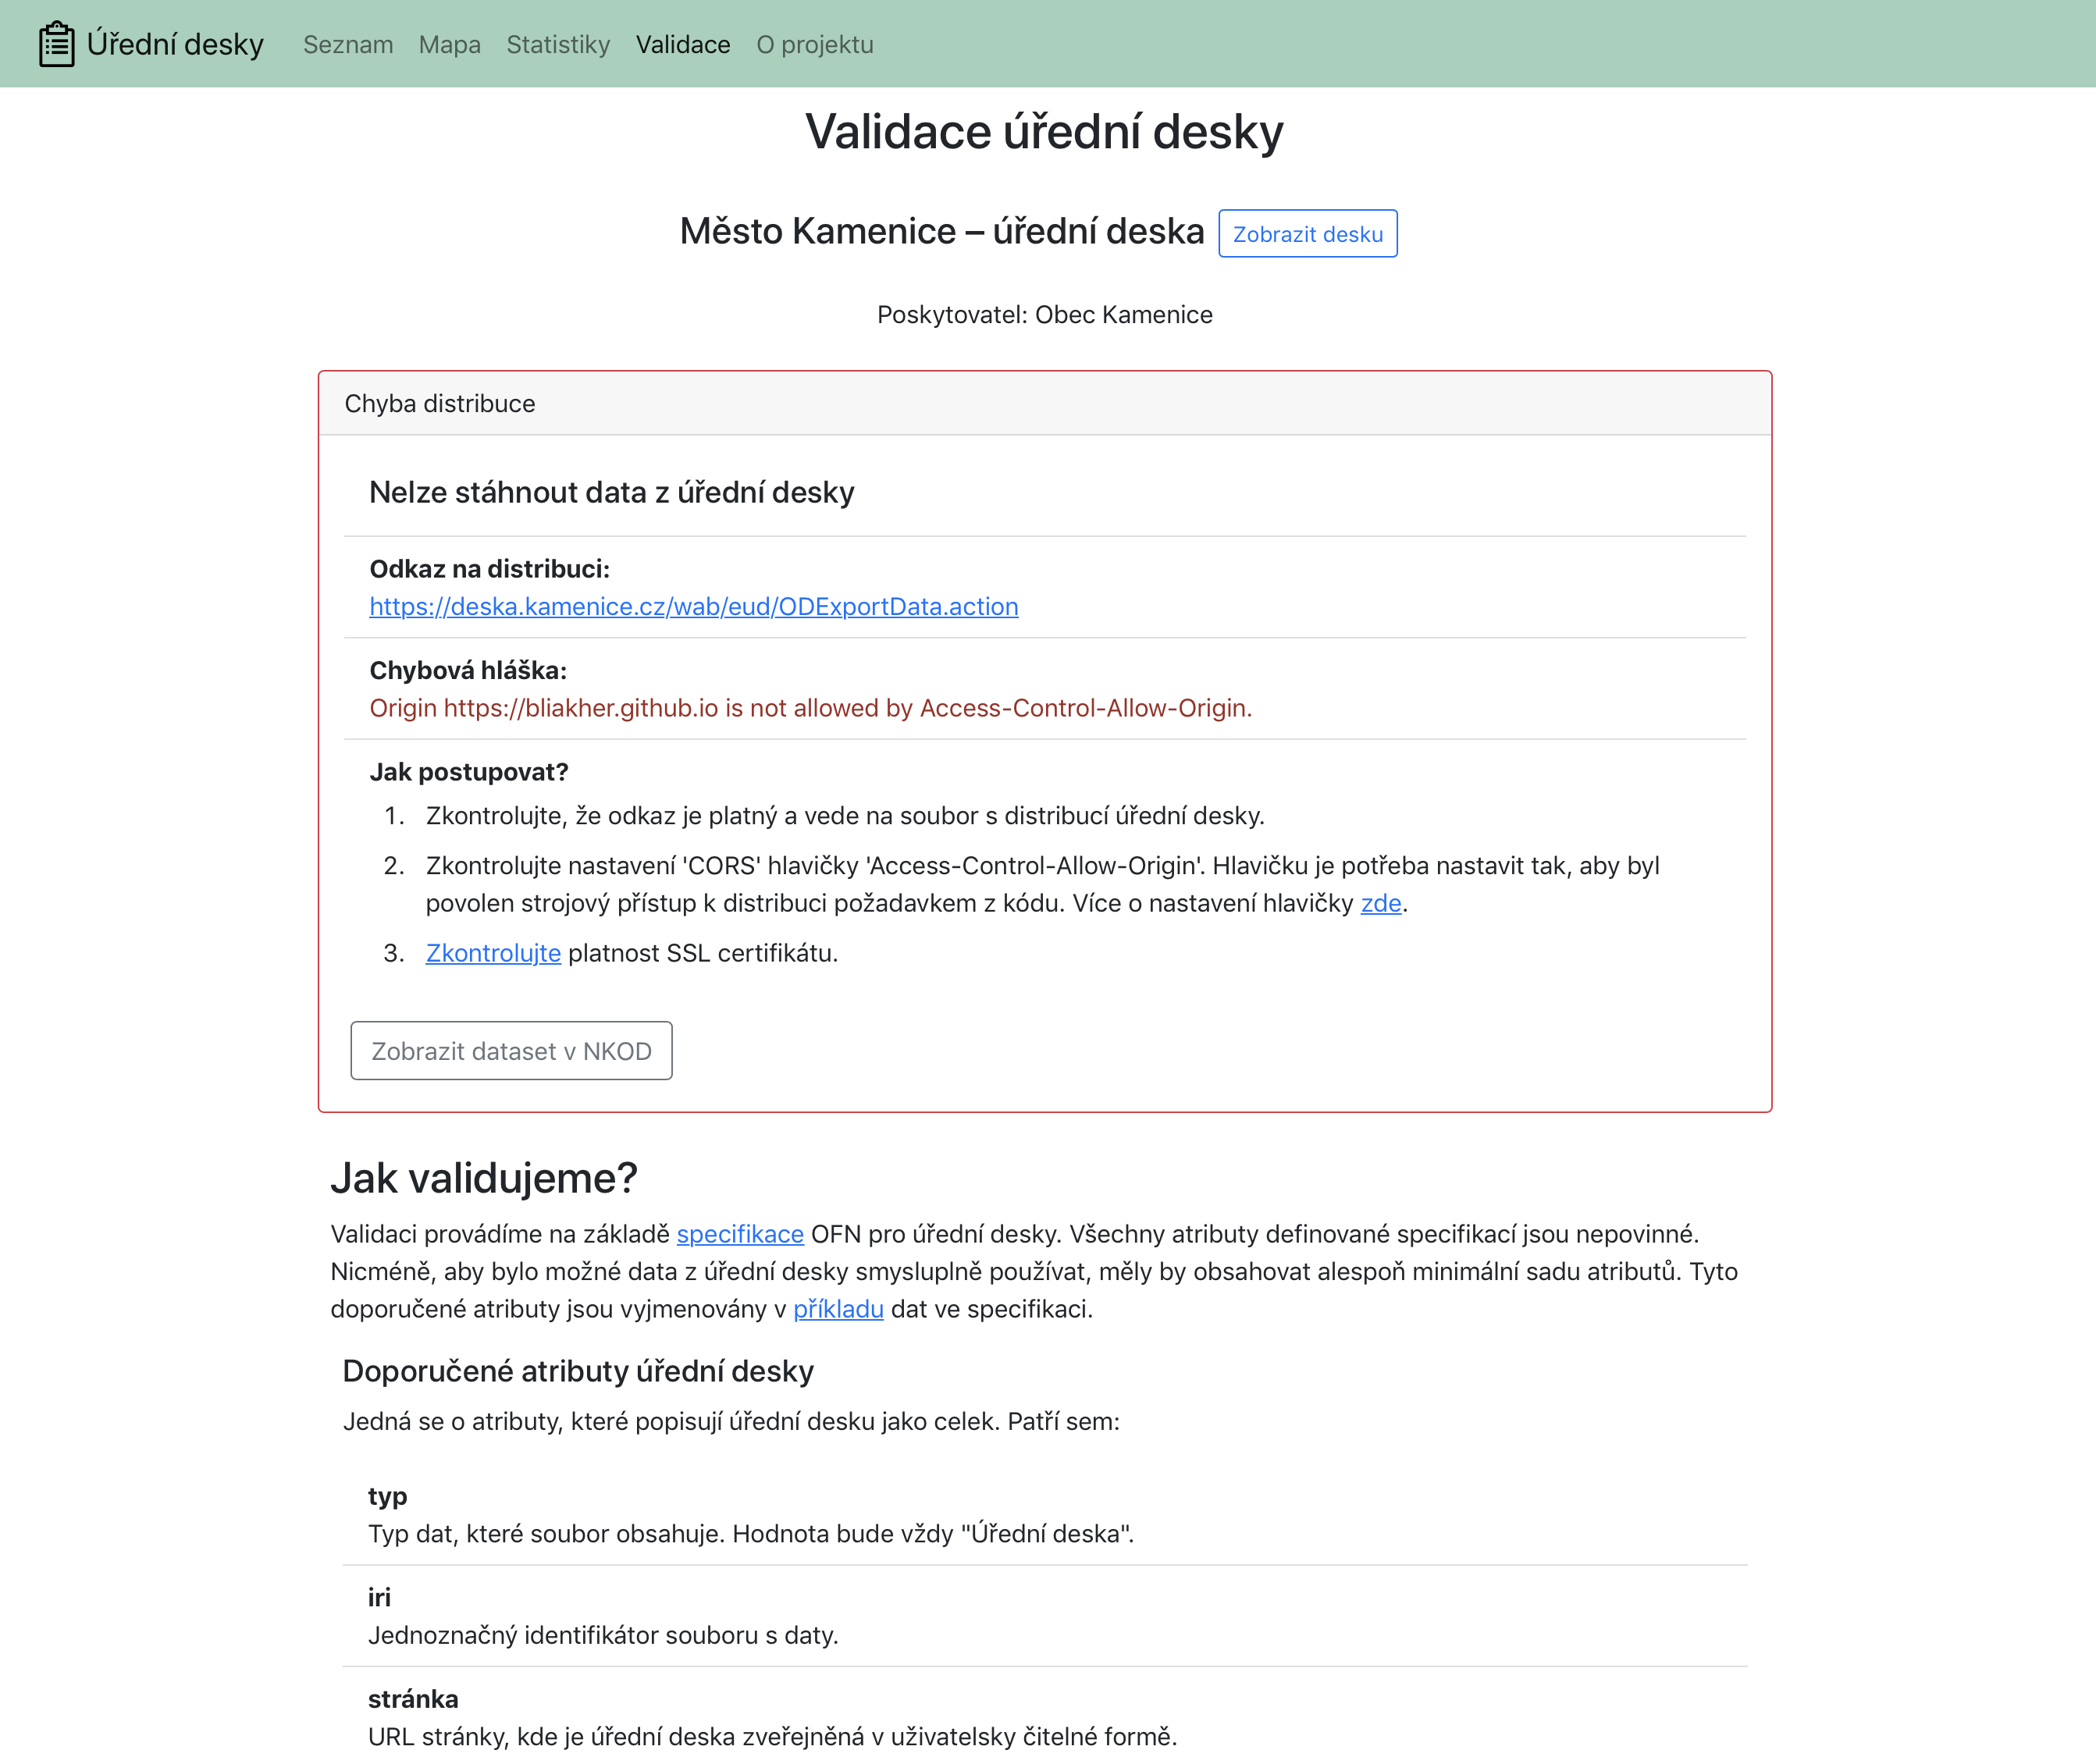
\includegraphics[width=\textwidth]{cs/obrazky/screenshots/validace_detail_cerveny.png}
\caption{Ukázka detailu validace úřední desky, u které není možné stáhnout distribuci}
\label{fig:screen-validace-c}
\end{figure}

Pokud v distribuci desky chybí některé doporučené atributy, je zde
vypsané, které to jsou. Pokud se jedná o doporučené atributy informací,
zobrazí se v záložce \textit{Informace\ s\ chybějícími\ atributy} seznam
všech informací s nedostatky, kde u každé informace je uvedeno, které
atributy chybí.

Na následujícím příkladu (\autoref{fig:screen-validace-z}) validace desky úřadu městské části Praha 5 si
můžeme všimnout, že v distribuci chybí doporučený atribut desky
\texttt{provozovatel} a v 10 informacích na desce z celkem 144 chybí
doporučený atribut \texttt{relevantní\_do}. Můžeme si prohlédnout, o
které informace se jedná.

\begin{figure}
\centering
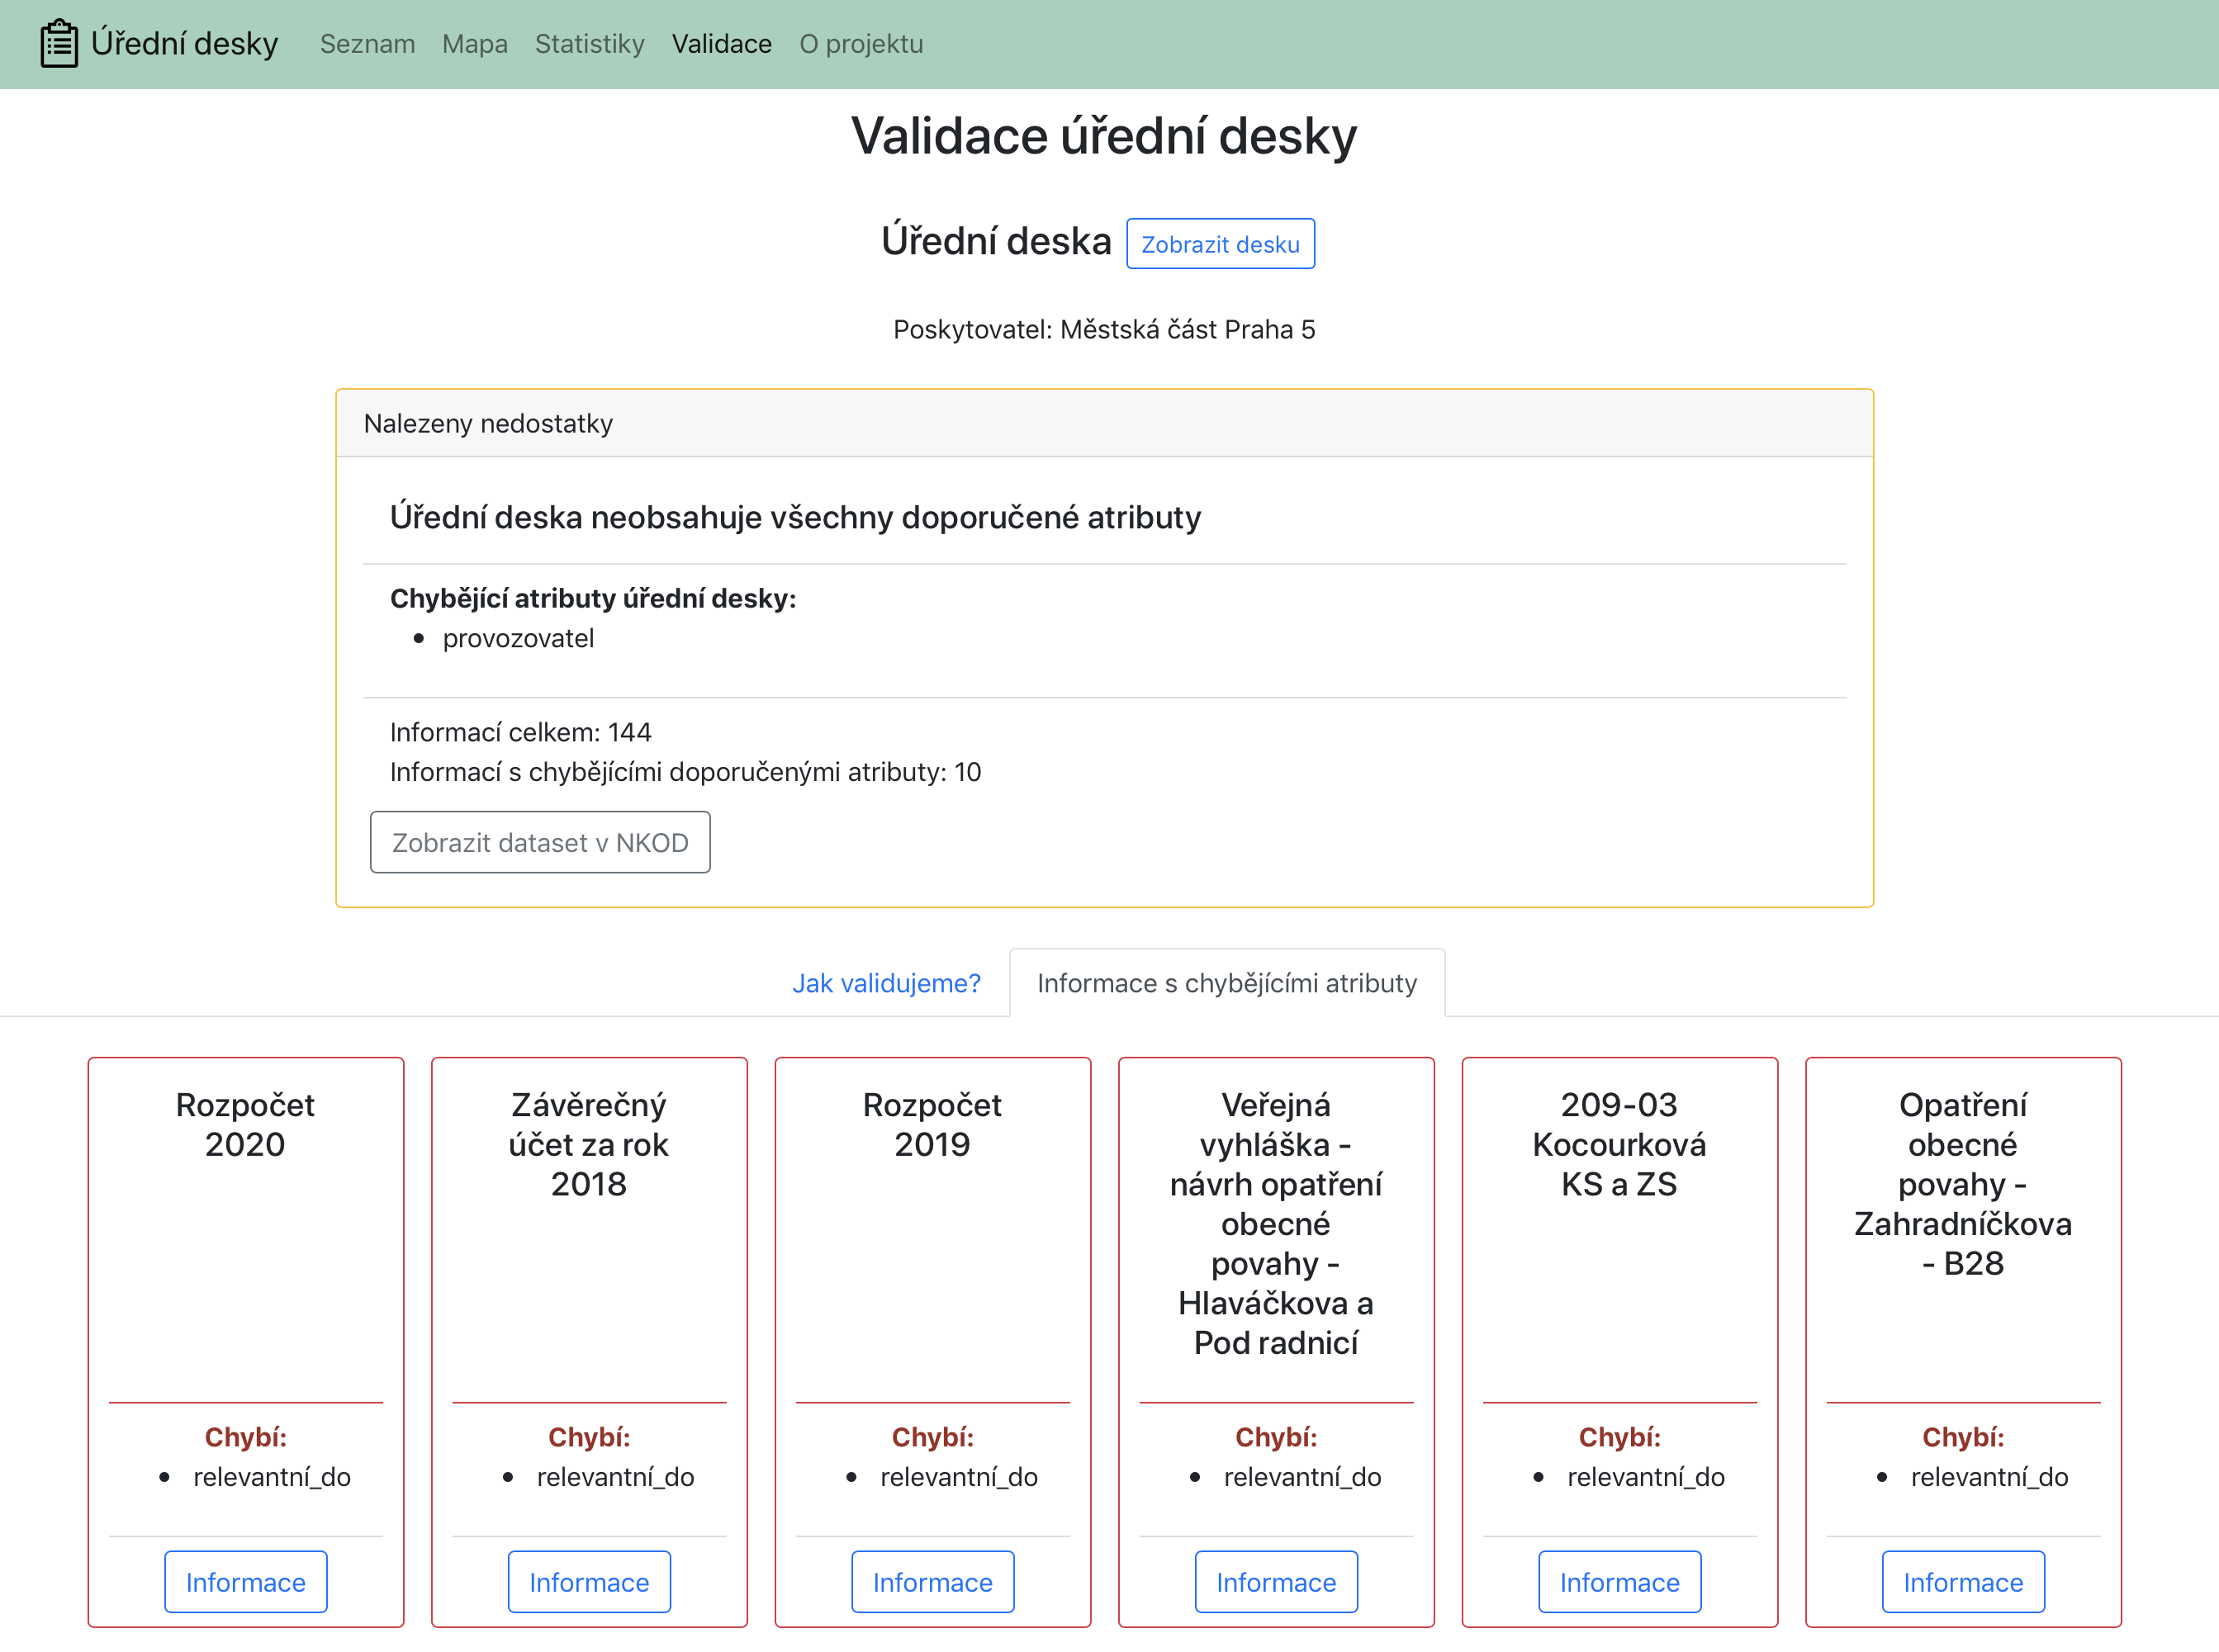
\includegraphics[width=\textwidth]{cs/obrazky/screenshots/validace_detail_zluty.png}
\caption{Ukázka detailu validace úřední desky, u které chybí některé doporučené atributy}
\label{fig:screen-validace-z}
\end{figure}

\subsection*{Statistiky}\label{statistiky}

V této části se zobrazují souhrnné statistiky výsledků validace a
poskytovatelů. Část Statistiky je rozdělená na 2 záložky --- \textit{Validace} a \textit{Poskytovatelé}.

V záložce \textit{Validace} jsou zobrazeny souhrnné výsledky validace v textové podobě a na koláčovém grafu. Jsou zde také seznamy desek, které obsahují nedostatky, ze kterých je možné se prokliknout na detail jejich validace.

Příklad validační statistiky vidíme na obrázku \ref{fig:screen-stat-val}.

\begin{figure}
\centering
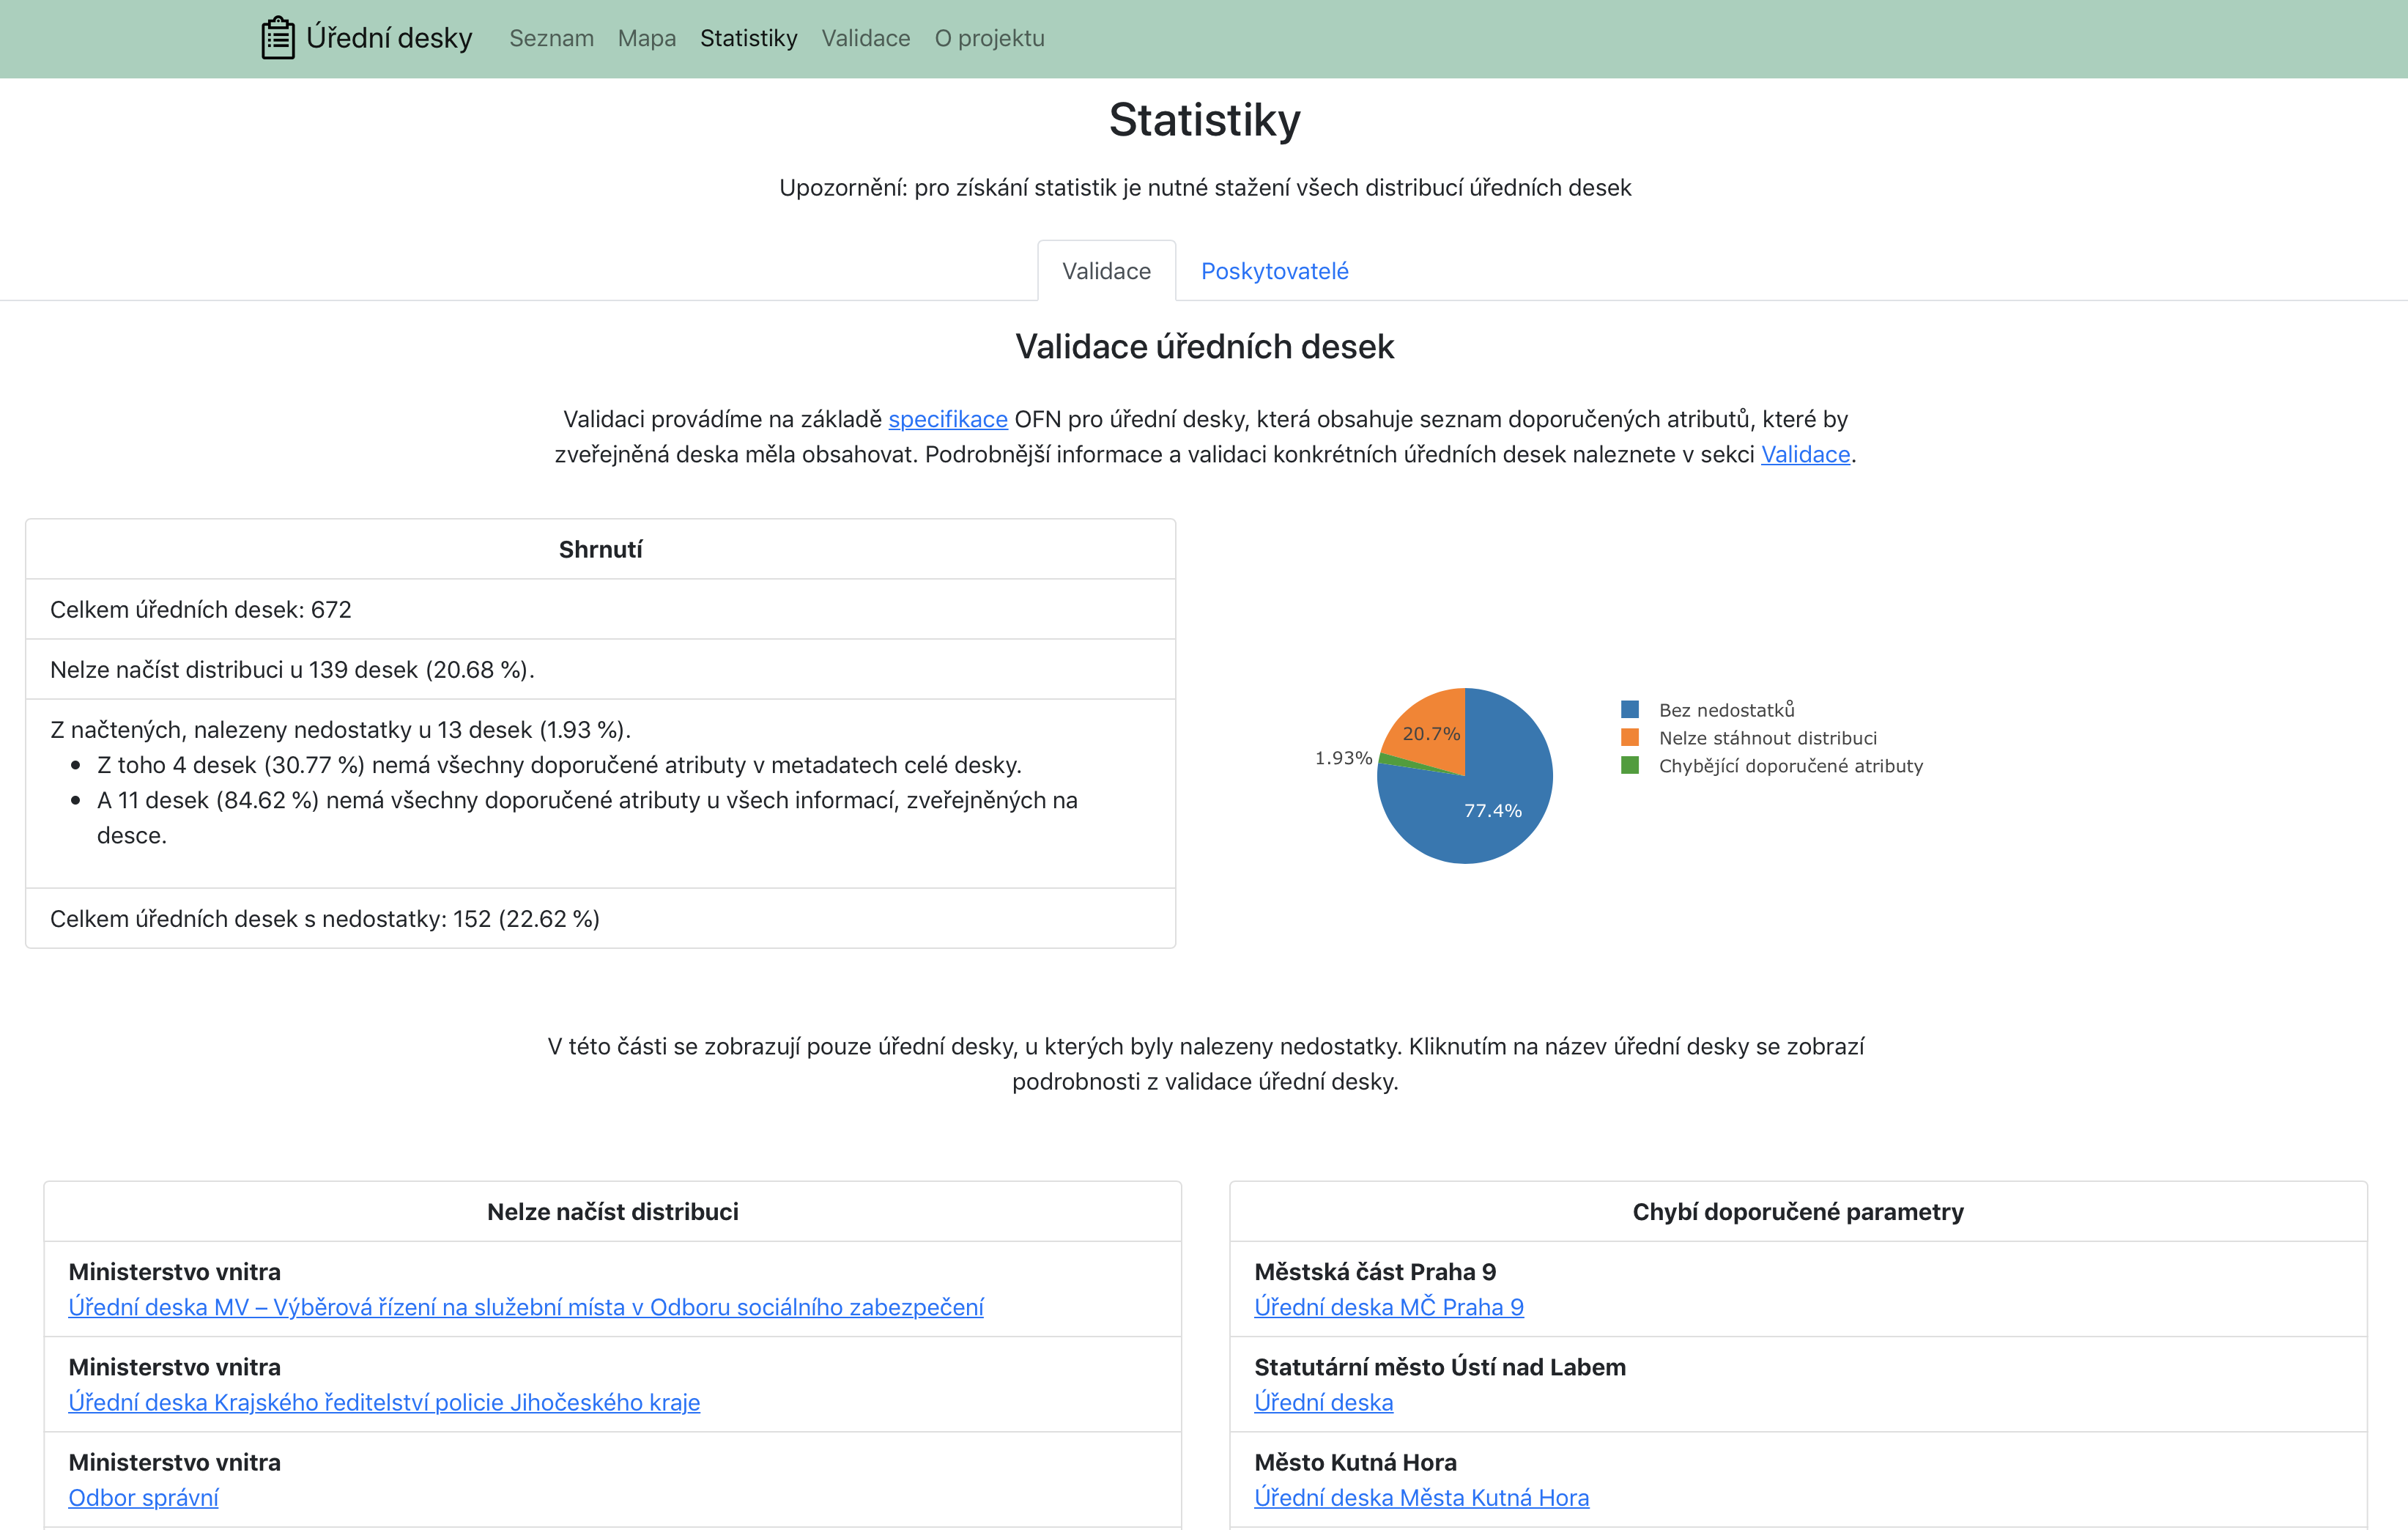
\includegraphics[width=\textwidth]{cs/obrazky/screenshots/statistika_validace.png}
\caption{Ukázka validační statistiky}
\label{fig:screen-stat-val}
\end{figure}

V záložce \textit{Poskytovatelé} je statistika poskytovatelů. Je zde zobrazeno, pro jednotlivé právní formy, kolik je celkem orgánů dané právní formy a kolik z nich poskytuje data ze svých úředních desek jako otevřená data. Pro největší skupiny poskytovatelů je toto zobrazeno na koláčových grafech a pro ostatní skupiny v textovém seznamu.

\begin{figure}
\centering
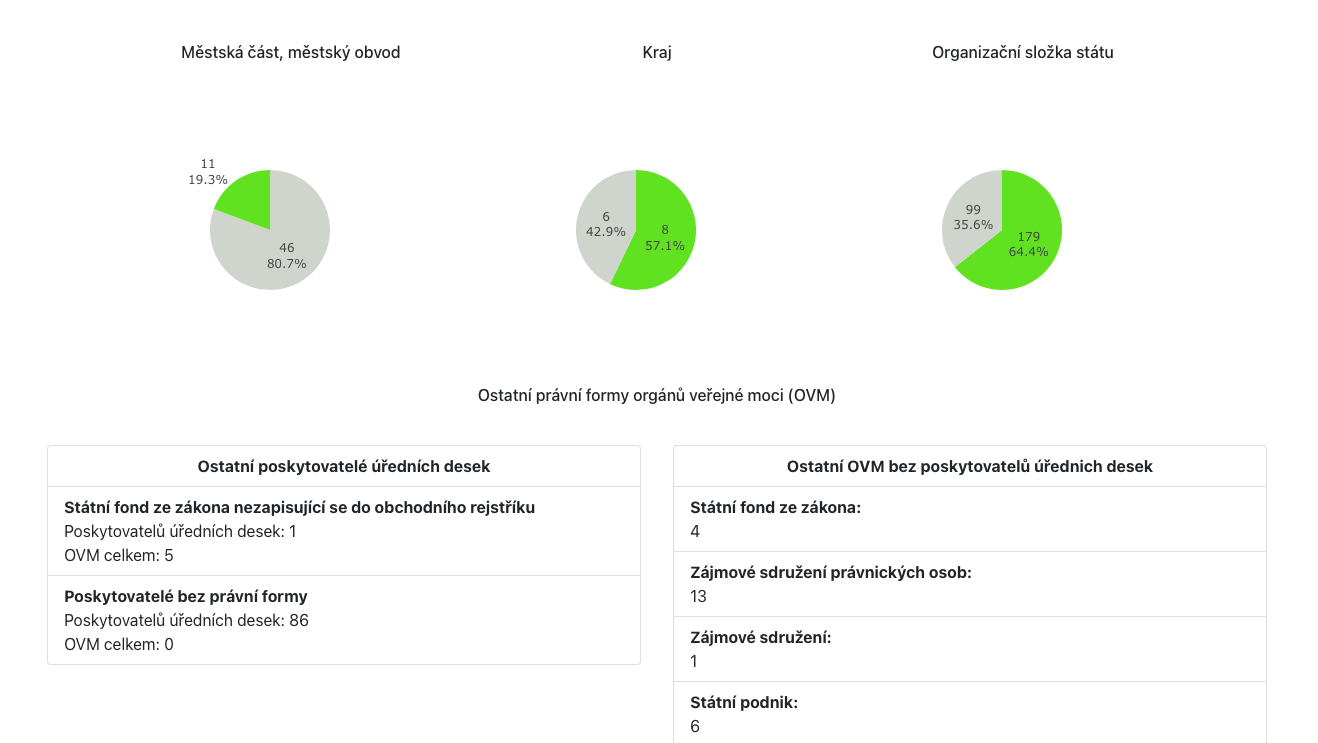
\includegraphics[width=\textwidth]{cs/obrazky/screenshots/statistika_poskytovatele.png}
\caption{Ukázka statistiky poskytovatelů}
\label{fig:screen-stat-posk}
\end{figure}

Na obrázku \ref{fig:screen-stat-posk} vidíme část statistiky poskytovatelů, konkrétně grafy pro městské
části, kraje a organizační složky státu. Pod nimi jsou 2 seznamy, v
prvním jsou poskytovatelé ostatních právních forem. Můžeme si všimnout,
že pro 86 poskytovatelů se nepodařilo zjistit jejich právní formu, což
nejspíše znamená, že tito poskytovatelé nemají svoji právní formu
uvedenou v
\href{https://www.szrcr.cz/cs/registr-prav-a-povinnosti}{Registru práv a
povinností}, odkud data o poskytovatelích získáváme.

Ve druhém seznamu jsou právní formy, které nemají žádného poskytovatele
úředních desek. U každé formy je uvedený celkový počet orgánů této
právní formy.


\section{Vývojářská dokumentace}\label{sec:developer-docs}

Vývojářská dokumentace je dostupná online na \url{https://bliakher.github.io/uredni_desky_docs/vyvojarska/}.

Vývojářská dokumentace obsahuje adresářovou strukturu repozitáře, popis vzájemného fungování různých částí aplikace a popis vybraných tříd a rozhraní. Je zde možné najít také dokumentaci všech tříd a rozhraní v aplikaci, vygenerovanou z komentářů v kódu pomocí nástroje TypeDoc \footnote{\url{https://typedoc.org/}}.


\section{Administrátorská dokumentace}\label{sec:admin-docs}

Administrátorská dokumentace je dostupná online na \url{https://bliakher.github.io/uredni_desky_docs/administratorska/}.

Obsahuje seznam požadavků a instrukce pro sestavení a nasazení aplikace.



\chapter{Evaluace}\label{kap:evaluace}

V této kapitole popíšeme uživatelské testování a celkovou evaluaci aplikace.

\section{Uživatelské testování}

Uživatelské testování bylo směřováno hlavně na uživatele s rolí veřejnost (viz uživatelské role popsané v části \ref{sec:role}), protože tento typ uživatelů bylo možné pro testování získat.

Testování jsme provedli podle metodiky System Usability Scale (SUS) \footnote{\url{https://www.usability.gov/how-to-and-tools/methods/system-usability-scale.html}}, která se používá ke zhodnocení použitelnosti uživatelských rozhraní aplikací. Uživatelé byli nejdříve seznámeni s účelem a základním fungováním aplikace. Poté měli projít 3 testovací scénáře, které jsou založené na případech užití pro roli veřejnost. Scénáře jsou podrobněji popsané v části \ref{sub:test-cases}. 

Nakonec měli ohodnotit, jak dobře se s aplikací pracuje v 10 standardizovaných otázkách z metodiky SUS. Každá otázka obsahovala tvrzení, na které bylo možné odpovědět jedním z 5 stupni souhlasu od zcela nesouhlasím k určitě souhlasím. Dotazník obsahoval tvrzení jako:
\begin{itemize}
    \item Systém mi přišel příliš složitý.
    \item Systém mi přišel snadno použitelný.
    \item Přišlo mi, že různé funkce tohoto systému jsou dobře integrovány.
    \item Při používání systému jsem se cítil(a) že vím co dělám.
\end{itemize}
Uživatele jsme také požádali o zpětnou vazbu a návrhy na vylepšení aplikace.

\subsection{Testovací scénáře}\label{sub:test-cases}

Uživatelé měli během testování projít 3 testovací scénáře, které jsou založené na případech užití, které patří k roli veřejnost. Na obrázku \ref{fig:use-cases-verejnost} vidíme část diagramu případů užití, kde jsou vybrané pouze ty případy užití, které se týkají uživatelů s rolí veřejnost. Všechny případy užití jsou popsané v části \ref{sec:use-cases}.

\begin{figure} 
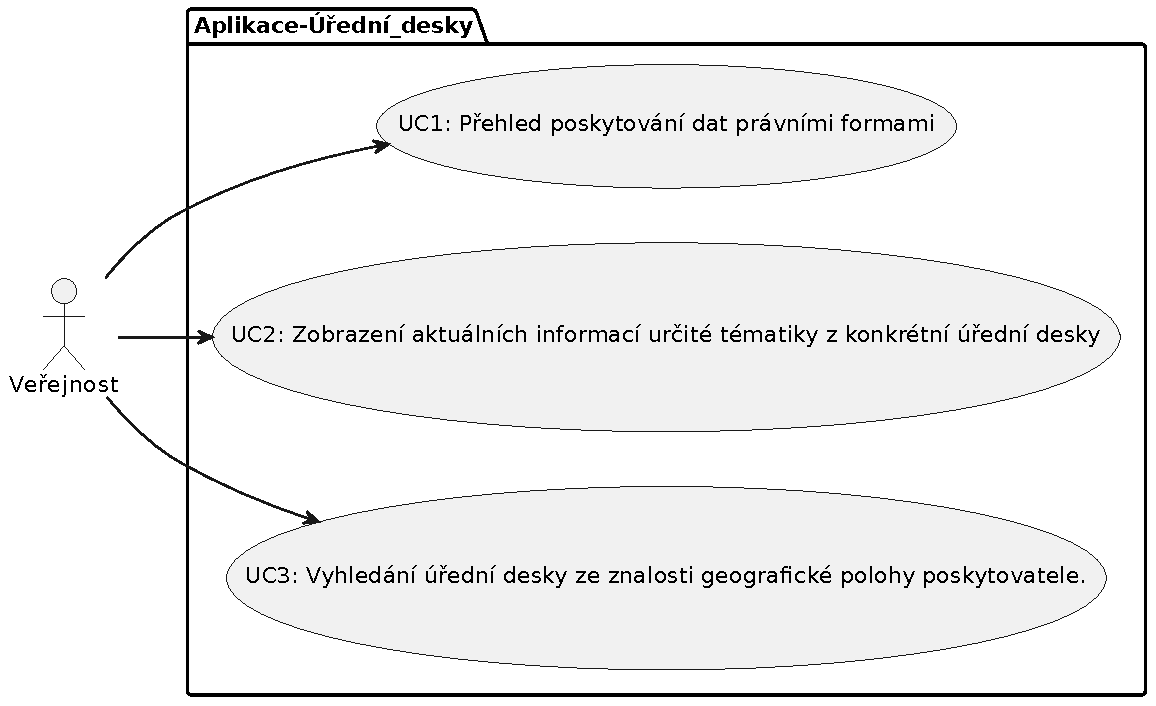
\includegraphics[width=\textwidth]{cs/obrazky/use-case-diagram-verejnost.pdf}
\caption{Diagram případů užití --- veřejnost}
\label{fig:use-cases-verejnost}
\end{figure}

Pro tyto případy užití byly navrženy následující testovací scénáře.

\subsubsection{Zobrazení aktuálních informací určité tématiky z konkrétní úřední desky}

Chceme najít informace, které se týkají dražeb v Městské části Praha 12.
\begin{enumerate}
    \item Otevřete aplikaci z odkazu: 
    \url{https://bliakher.github.io/uredni_desky}. Měla by se otevřít stránka se seznamem všech úředních desek.
    \item Pomocí formuláře pro vyhledávání najděte úřední desku Městské části Praha 12.
    \item Otevřete detail desky kliknutím na tlačítko \textit{Zobrazit informace}.
    \item Nyní byste měli vidět všechny informace vyvěšené na této desce.
    \item Použijte formulář na vyhledávání v informacích k nalezení informací, které se týkají dražeb.
    \item Prohlédněte si informace o dražbách.
\end{enumerate}

\subsubsection{Přehled poskytování dat právními formami}

Chceme zjistit, které krajské úřady poskytují svoji úřední desku.
\begin{enumerate}
    \item V aplikaci se vraťte na seznam úředních desek kliknutím na \textit{Seznam} v navigačním panelu.
    \item Vyfiltrujte pouze ty desky, jejichž poskytovatelem je krajský úřad. To uděláte pomocí panelu \textit{Vyberte právní formu poskytovatele}, kde necháte vybranou pouze právní formu Kraje.
    \item V seznamu by měly zůstat pouze úřední desky krajů.
    \item Prohlédněte si, které kraje poskytují svoji úřední desku.
\end{enumerate}

\subsubsection{Vyhledání úřední desky ze znalosti geografické polohy poskytovatele.}

Chceme najít úřední desky v okolí.
\begin{enumerate}
    \item  V aplikaci přejděte do části s mapou kliknutím na \textit{Mapa} v navigačním panelu.
    \item  Měla by se vám zobrazit mapa ČR, na kterém jsou body vyznačená sídla poskytovatelů úředních desek. Když kliknete na nějaký bod, zobrazí se vám úřední desky daného poskytovatele.
    \item Najděte na mapě obec, ve které bydlíte.
    \item Zjistěte, jestli vaše obec nebo váš krajský úřad poskytuje úřední desku, případně jaké obce v okolí ji poskytují.
\end{enumerate}


\subsection{Výsledky testování}\label{sub:vysledky-testovani}

Testování se zúčastnilo 11 uživatelů. Získali jsme následující výsledky.

Většina uživatelů se shodla na tom, že systém není příliš složitý a naopak je snadno použitelný. Uživatelé při používání systému cítí, že ví, co dělají a nepotřebují podporu technického personálu.

Někteří uživatelé hodnotili systém jako těžkopádný. Na tvrzení: \textit{``Systém mi přišel velice těžkopádný.''} odpovědělo 6 uživatelů \textit{určitě nesouhlasím}, 3 \textit{spíše nesouhlasím} a 2 \textit{spíše souhlasím}.

Několika uživatelům přišla aplikace v něčem nekonzistentní. Na tvrzení: \textit{``Přišlo mi, že je systém příliš nekonzistentní (rozdílné názvy pro stejné věci, rozdílné ovládání podobných prvků...)''} odpovědělo 7 uživatelů \textit{určitě nesouhlasím}, 2 \textit{spíše nesouhlasím}, 1 \textit{nemám názor} a 1 \textit{spíše souhlasím}.

Všechny odpovědi uživatelů v testování shromážděné podle tvrzení je možné najít v tabulce v příloze \ref{fig:testovani-vysledky}. 

Podle metodiky SUS bylo pro každého uživatele vypočítané skóre aplikace. Výsledky je možné najít v příloze \ref{fig:testovani-skore}. Pokud má skóre hodnotu vyšší než 68, můžeme to podle metodiky interpretovat tak, že je aplikace z hlediska použitelnosti lepší než průměrná aplikace. Průměrné skóre aplikace vyšlo 87,05.

Kromě výsledků dotazníku, jsme od uživatelů také získali zpětnou vazbu k aplikaci.

Na doporučení uživatelů byly barevně zvýrazněné některé prvky, které jsou důležité pro navigaci v aplikaci, jako například tlačítko \textit{Zobrazit informace}, které umožňuje přejít ze seznamu do detailu desky. Také bylo přidáno navigační tlačítko \textit{Zpět}, které slouží pro návrat z detailu vizualizace nebo validace zpět do seznamu.

Jako možná vylepšení aplikace uživatelé zmiňovali přidání našeptávání ve formulářích pro vyhledávání.

\section{Evaluace --- poskytovatelé dat}

Aplikaci jsme rozeslali několika představitelům úřadů, které jsou poskytovateli dat z úředních desek. Byl vysvětlen účel a základní fungování aplikace a poskytovatelé dat byli požádáni o zpětnou vazbu k fungování aplikace z jejich pohledu.

Poskytovatelé hodnotili aplikaci pozitivně. Jako možná vylepšení navrhovali v části vizualizace desky rozdělení informací tématicky (např. doprava, výstavba, volby). Toto je teoreticky proveditelné pomocí atributu \texttt{agenda} \footnote{\url{https://ofn.gov.cz/úřední-desky/2021-07-20/\#vazba-informace-agenda}}, který je možné přidat k informaci na úřední desce podle OFN pro úřední desky. Tento atribut ale není mezi doporučenými atributy a ne všichni poskytovatelé ho používají.

V části validace byl návrh na přidání více možností pro filtrování tabulky, které by bylo zabudované do hlavičky tabulky --- mohlo by se jednat například o abecední řazení nebo řazení podle počtu informací na desce. 



\chapter*{Závěr}
\addcontentsline{toc}{chapter}{Závěr}

V rámci bakalářské práce byly analyzovány existující aplikace pro prohlížení úředních desek. Také byly prozkoumány možnosti, které nabízí zveřejňování dat z úředních desek jako otevřených dat podle OFN pro úřední desky. Na základě analýzy byly sestaveny požadavky na aplikaci, která by pracovala s daty z úředních desek zveřejněných v NKOD jako otevřená data a umožňovala by jejich vizualizaci a validaci.

Podle požadavků byl proveden návrh a následně implementace aplikace. Aplikace umožňuje přehledně prohlížet a vyhledávat informace na úředních deskách. Z pohledu poskytovatele dat stačí data zveřejnit v NKOD a není potřeba žádná další činnost proto, aby byla data vizualizována aplikací. Aplikace také poskytovatelům nabízí validaci dat podle specifikace OFN, včetně vysvětlení významu dat a řešení nejčastějších problémů se zveřejněním dat.

Aplikace propojuje data z úředních desek s informacemi o jejich poskytovatelích, získanými z dalších registrů otevřených dat, což umožňuje vizualizovat úřední desky na mapě a zobrazit statistický přehled poskytovatelů dat.

Aplikace byla otestována v uživatelském testování, kde ji uživatelé ohodnotili jako snadno použitelnou. Na základě podnětů od uživatelů byly vylepšené některé prvky v uživatelském rozhraní.

Aplikaci je možné dále vylepšovat. Některé návrhy na rozšíření byly popsané ve zpětné vazbě uživatelů k testování, \autoref{sub:vysledky-testovani}. 

Dalším možným rozšířením je vyhledávání a filtrování informací napříč všemi úředními deskami, nebo nějakou vybranou skupinou desek. Aplikace zatím umožňuje pouze vyhledávání informací v rámci jedné desky. Toto rozšíření v současné době neumožňuje architektura aplikace, postavená na straně klienta (viz \autoref{sec:architektura}), což je dané požadavky na způsob nasazení aplikace (viz \autoref{sub:tech-poz}). Vyhledávání ve velkém množství informací na straně klienta by bylo velmi neefektivní.

%%% Seznam použité literatury
%%% Seznam použité literatury (bibliografie)
%%%
%%% Pro vytváření bibliografie používáme bibTeX. Ten zpracovává
%%% citace v textu (např. makro \cite{...}) a vyhledává k nim literaturu
%%% v souboru literatura.bib.
%%%
%%% Příkaz \bibliographystyle určuje, jakým stylem budou citovány odkazy
%%% v textu. V závorce je název zvoleného souboru .bst. Styly plainnat
%%% a unsrt jsou standardní součástí latexových distribucí. Styl czplainnat
%%% je dodáván s touto šablonou a bibTeX ho hledá v aktuálním adresáři.

%\bibliographystyle{czplainnat}    %% Autor (rok) s českými spojkami
% \bibliographystyle{plainnat}    %% Autor (rok) s anglickými spojkami
\bibliographystyle{unsrt}       %% [číslo]

\renewcommand{\bibname}{Seznam použité literatury}

%%% Vytvoření seznamu literatury. Pozor, pokud jste necitovali ani jednu
%%% položku, seznam se automaticky vynechá.

\bibliography{literatura}

%%% Kdybyste chtěli bibliografii vytvářet ručně (bez bibTeXu), lze to udělat
%%% následovně. V takovém případě se řiďte normou ISO 690 a zvyklostmi v oboru.

% \begin{thebibliography}{99}
%
% \bibitem{lamport94}
%   {\sc Lamport,} Leslie.
%   \emph{\LaTeX: A Document Preparation System}.
%   2. vydání.
%   Massachusetts: Addison Wesley, 1994.
%   ISBN 0-201-52983-1.
%
% \end{thebibliography}


%%% Obrázky v bakalářské práci
%%% (pokud jich je malé množství, obvykle není třeba seznam uvádět)
\listoffigures

%%% Tabulky v bakalářské práci (opět nemusí být nutné uvádět)
%%% U matematických prací může být lepší přemístit seznam tabulek na začátek práce.
%\listoftables

%%% Použité zkratky v bakalářské práci (opět nemusí být nutné uvádět)
%%% U matematických prací může být lepší přemístit seznam zkratek na začátek práce.
\chapwithtoc{Seznam použitých zkratek}

\begin{itemize}
    \item[API] Application Programming Interface
    \item[ČR] Česká republika
    \item[DOM] Document Object Model
    \item[HTML] Hypertext Markup Language
    \item[HTTP] Hypertext Transfer Protocol
    \item[IRI] Internationalized Resource Identifier
    \item[IČO] Identifikační číslo osoby
    \item[JSON] JavaScript Object Notation
    \item[JSON-LD] JavaScript Object Notation for Linked Data
    \item[JSX] JavaScript Syntax Extension, JavaScript XML
    \item[MFF UK] Matematicko-fyzikální fakulta Univerzity Karlovy
    \item[NKOD] Národní katalog otevřených dat
    \item[OFN] Otevřená formální norma
    \item[OVM] Orgán veřejné moci
    \item[RDF] Resource Description Framework
    \item[RPP] Registr práv a povinností
    \item[RÚIAN] Registr územní identifikace, adres a nemovitostí
    \item[SPARQL] SPARQL Protocol and RDF Query Language
    \item[SUS] System Usability Scale
    \item[URL] Uniform Resource Locator
    \item[XML] Extensible Markup Language
    
\end{itemize}







%%% Přílohy k bakalářské práci, existují-li. Každá příloha musí být alespoň jednou
%%% odkazována z vlastního textu práce. Přílohy se číslují.
%%%
%%% Do tištěné verze se spíše hodí přílohy, které lze číst a prohlížet (dodatečné
%%% tabulky a grafy, různé textové doplňky, ukázky výstupů z počítačových programů,
%%% apod.). Do elektronické verze se hodí přílohy, které budou spíše používány
%%% v elektronické podobě než čteny (zdrojové kódy programů, datové soubory,
%%% interaktivní grafy apod.). Elektronické přílohy se nahrávají do SISu a lze
%%% je také do práce vložit na CD/DVD. Povolené formáty souborů specifikuje
%%% opatření rektora č. 72/2017.
\appendix
\chapter{Přílohy}

\section{Výsledky uživatelského testování}

V této části jsou tabulky s výsledky uživatelského testování podle metodiky System Usability Scale (SUS)\footnote{\url{https://www.usability.gov/how-to-and-tools/methods/system-usability-scale.html}}. Uživatele ve standartním dotazníku o 10 otázkách hodnotili použitelnost aplikace jedním z 5 stupni souhlasu od zcela nesouhlasím k určitě souhlasím. Tabulky jsme pro větší přehlednost umístili na šířku.

\subsection{Počty odpovědí podle otázek}

V tabulce \ref{table:vysledky1} jsou počty jednotlivých odpovědí pro každou otázku.  

% \begin{figure}
%     \centering
%     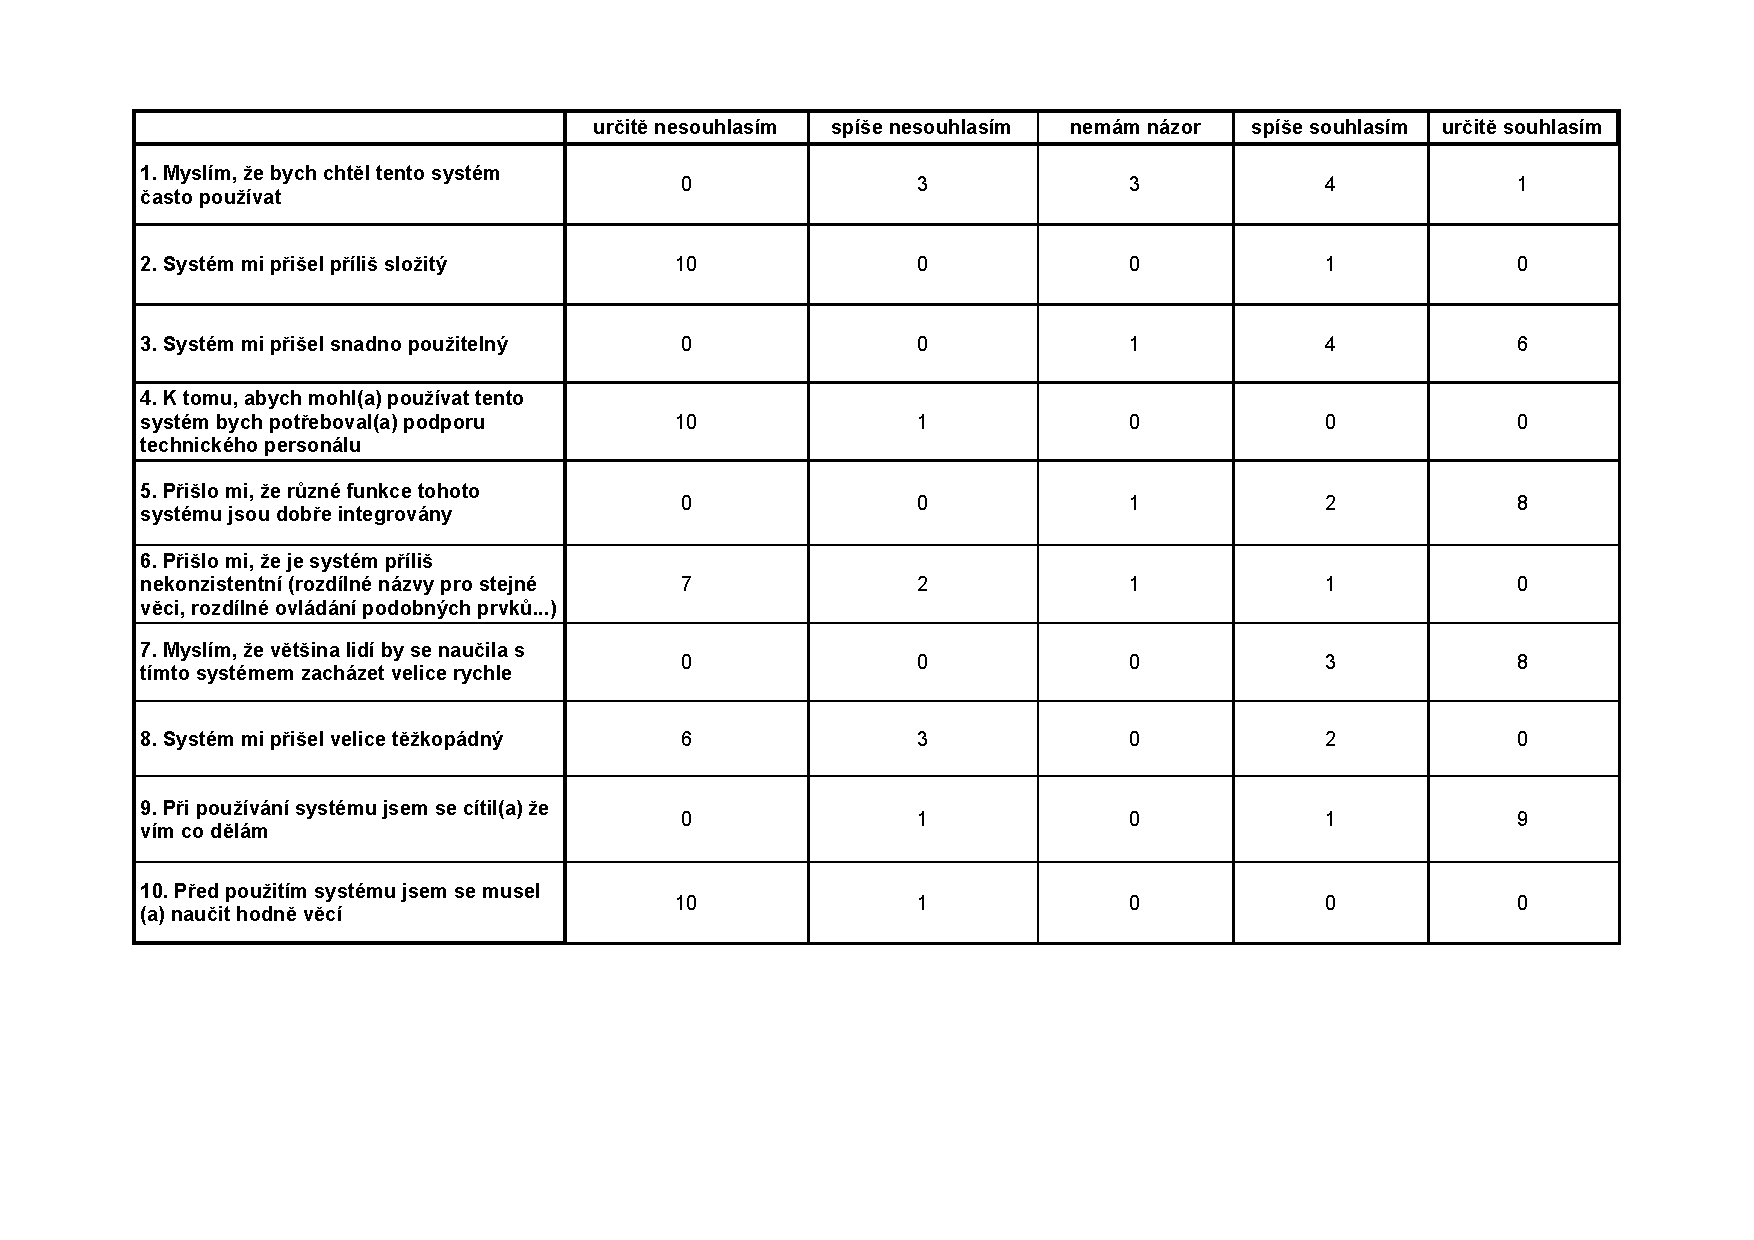
\includegraphics[width=1.4\textwidth, angle=-90]{cs/prilohy/uzivatelske_testovani_vysledky.pdf}
%     \caption{Výsledky uživatelského testování podle SUS}
%     \label{fig:testovani-vysledky}
% \end{figure}

\begin{sidewaystable}[]
\centering
\begin{tabular}{|l|c|c|c|c|c|}
\hline
\textbf{Tvrzení}                                                                                                                                                               & \textbf{\begin{tabular}[c]{@{}c@{}}určitě \\ nesouhlasím\end{tabular}} & \textbf{\begin{tabular}[c]{@{}c@{}}spíše\\  nesouhlasím\end{tabular}} & \textbf{\begin{tabular}[c]{@{}c@{}}nemám\\ názor\end{tabular}} & \textbf{\begin{tabular}[c]{@{}c@{}}spíše\\ souhlasím\end{tabular}} & \textbf{\begin{tabular}[c]{@{}c@{}}určitě\\ souhlasím\end{tabular}} \\ \hline
\textbf{1. Myslím, že bych chtěl tento systém často používat}                                                                                                                  & 0                                                                      & 3                                                                     & 3                                                              & 4                                                                  & 1                                                                   \\ \hline
\textbf{2. Systém mi přišel příliš složitý}                                                                                                                                    & 10                                                                     & 0                                                                     & 0                                                              & 1                                                                  & 0                                                                   \\ \hline
\textbf{3. Systém mi přišel snadno použitelný}                                                                                                                                 & 0                                                                      & 0                                                                     & 1                                                              & 4                                                                  & 6                                                                   \\ \hline
\textbf{\begin{tabular}[c]{@{}l@{}}4. K tomu, abych mohl(a) používat tento systém\\ bych potřeboval(a) podporu technického personálu\end{tabular}}                             & 10                                                                     & 1                                                                     & 0                                                              & 0                                                                  & 0                                                                   \\ \hline
\textbf{\begin{tabular}[c]{@{}l@{}}5. Přišlo mi, že různé funkce tohoto systému jsou\\ dobře integrovány\end{tabular}}                                                         & 0                                                                      & 0                                                                     & 1                                                              & 2                                                                  & 8                                                                   \\ \hline
\textbf{\begin{tabular}[c]{@{}l@{}}6. Přišlo mi, že je systém příliš nekonzistentní \\ (rozdílné názvy pro stejné věci, \\ rozdílné ovládání podobných prvků...)\end{tabular}} & 7                                                                      & 2                                                                     & 1                                                              & 1                                                                  & 0                                                                   \\ \hline
\textbf{\begin{tabular}[c]{@{}l@{}}7. Myslím, že většina lidí by se naučila s tímto\\  systémem zacházet velice rychle\end{tabular}}                                           & 0                                                                      & 0                                                                     & 0                                                              & 3                                                                  & 8                                                                   \\ \hline
\textbf{8. Systém mi přišel velice těžkopádný}                                                                                                                                 & 6                                                                      & 3                                                                     & 0                                                              & 2                                                                  & 0                                                                   \\ \hline
\textbf{9. Při používání systému jsem se cítil(a) že vím co dělám}                                                                                                             & 0                                                                      & 1                                                                     & 0                                                              & 1                                                                  & 9                                                                   \\ \hline
\textbf{\begin{tabular}[c]{@{}l@{}}10. Před použitím systému jsem se musel(a) \\ naučit hodně věcí\end{tabular}}                                                               & 10                                                                     & 1                                                                     & 0                                                              & 0                                                                  & 0                                                                   \\ \hline
\end{tabular}
\caption{Výsledky uživatelského testování - podle otázek}
\label{table:vysledky1}
\end{sidewaystable}

\subsection{Odpovědi a skóre podle uživatelů}

V tabulce \ref{table:vysledky2} jsou vypsané odpovědi jednotlivých uživatelů a pro každého je spočítané výsledné skóre.

% \begin{figure}
%     \centering
%     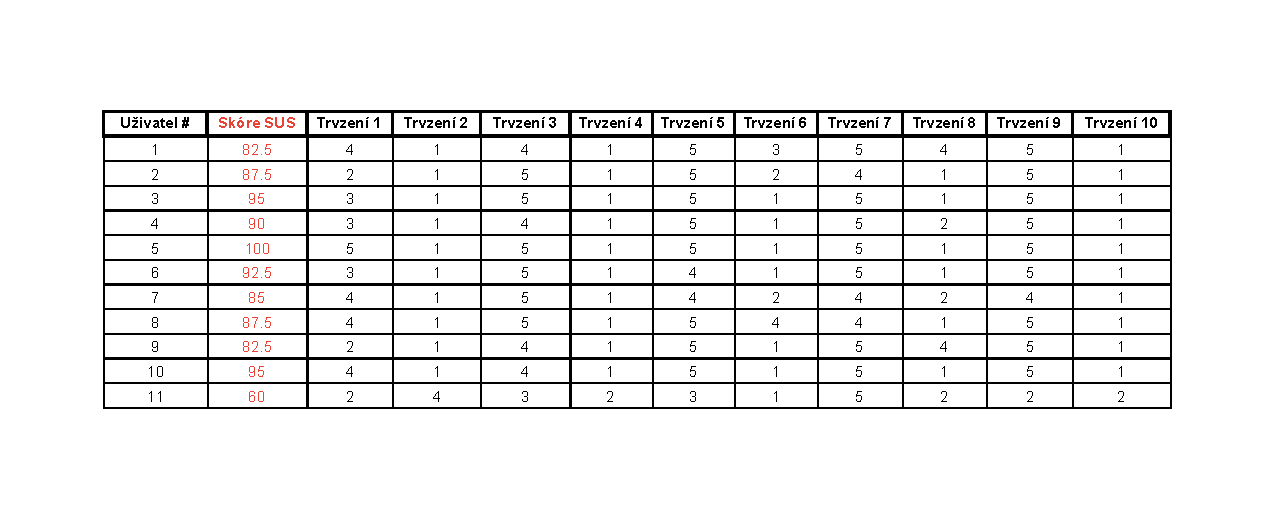
\includegraphics[width=1.6\textwidth, angle=-90]{cs/prilohy/skoreSUS2.pdf}
%     \caption{Skóre SUS pro jednotlivé uživatele}
%     \label{fig:testovani-skore}
% \end{figure}

\begin{sidewaystable}
\centering
\begin{tabular}{|c|c|c|c|c|c|c|c|c|c|c|c|}
\hline
\textbf{\begin{tabular}[c]{@{}c@{}}Uživatel \\ \#\end{tabular}} & {\color[HTML]{EA4335} \textbf{\begin{tabular}[c]{@{}c@{}}Skóre\\  SUS\end{tabular}}} & \textbf{\begin{tabular}[c]{@{}c@{}}Trvzení\\ 1\end{tabular}} & \textbf{\begin{tabular}[c]{@{}c@{}}Trvzení\\ 2\end{tabular}} & \textbf{\begin{tabular}[c]{@{}c@{}}Trvzení\\ 3\end{tabular}} & \textbf{\begin{tabular}[c]{@{}c@{}}Trvzení\\ 4\end{tabular}} & \textbf{\begin{tabular}[c]{@{}c@{}}Trvzení\\ 5\end{tabular}} & \textbf{\begin{tabular}[c]{@{}c@{}}Trvzení\\ 6\end{tabular}} & \textbf{\begin{tabular}[c]{@{}c@{}}Trvzení\\ 7\end{tabular}} & \textbf{\begin{tabular}[c]{@{}c@{}}Trvzení\\ 8\end{tabular}} & \textbf{\begin{tabular}[c]{@{}c@{}}Trvzení\\ 9\end{tabular}} & \textbf{\begin{tabular}[c]{@{}c@{}}Trvzení\\ 10\end{tabular}} \\ \hline
1                                                               & {\color[HTML]{EA4335} 82.5}                                                          & 4                                                            & 1                                                            & 4                                                            & 1                                                            & 5                                                            & 3                                                            & 5                                                            & 4                                                            & 5                                                            & 1                                                             \\ \hline
2                                                               & {\color[HTML]{EA4335} 87.5}                                                          & 2                                                            & 1                                                            & 5                                                            & 1                                                            & 5                                                            & 2                                                            & 4                                                            & 1                                                            & 5                                                            & 1                                                             \\ \hline
3                                                               & {\color[HTML]{EA4335} 95}                                                            & 3                                                            & 1                                                            & 5                                                            & 1                                                            & 5                                                            & 1                                                            & 5                                                            & 1                                                            & 5                                                            & 1                                                             \\ \hline
4                                                               & {\color[HTML]{EA4335} 90}                                                            & 3                                                            & 1                                                            & 4                                                            & 1                                                            & 5                                                            & 1                                                            & 5                                                            & 2                                                            & 5                                                            & 1                                                             \\ \hline
5                                                               & {\color[HTML]{EA4335} 100}                                                           & 5                                                            & 1                                                            & 5                                                            & 1                                                            & 5                                                            & 1                                                            & 5                                                            & 1                                                            & 5                                                            & 1                                                             \\ \hline
6                                                               & {\color[HTML]{EA4335} 92.5}                                                          & 3                                                            & 1                                                            & 5                                                            & 1                                                            & 4                                                            & 1                                                            & 5                                                            & 1                                                            & 5                                                            & 1                                                             \\ \hline
7                                                               & {\color[HTML]{EA4335} 85}                                                            & 4                                                            & 1                                                            & 5                                                            & 1                                                            & 4                                                            & 2                                                            & 4                                                            & 2                                                            & 4                                                            & 1                                                             \\ \hline
8                                                               & {\color[HTML]{EA4335} 87.5}                                                          & 4                                                            & 1                                                            & 5                                                            & 1                                                            & 5                                                            & 4                                                            & 4                                                            & 1                                                            & 5                                                            & 1                                                             \\ \hline
9                                                               & {\color[HTML]{EA4335} 82.5}                                                          & 2                                                            & 1                                                            & 4                                                            & 1                                                            & 5                                                            & 1                                                            & 5                                                            & 4                                                            & 5                                                            & 1                                                             \\ \hline
10                                                              & {\color[HTML]{EA4335} 95}                                                            & 4                                                            & 1                                                            & 4                                                            & 1                                                            & 5                                                            & 1                                                            & 5                                                            & 1                                                            & 5                                                            & 1                                                             \\ \hline
11                                                              & {\color[HTML]{EA4335} 60}                                                            & 2                                                            & 4                                                            & 3                                                            & 2                                                            & 3                                                            & 1                                                            & 5                                                            & 2                                                            & 2                                                            & 2                                                             \\ \hline
\end{tabular}
\caption{Výsledky uživatelského testování - podle uživatelů}
\label{table:vysledky2}
\end{sidewaystable}


\section{Repozitáře}

Přílohou práce jsou repozitáře se zdrojovým kódem aplikace a dokumentace. Stav repozitáře v momentě odevzdání práce je označen tagem \texttt{odevzdani}. Snapshot repozitářů z tohoto tagu je přiložený ve formátu ZIP.

\subsection{Repozitář \texttt{uredni\_desky}} \label{sub:repo1}

Repozitář \texttt{uredni\_desky} normálně přístupný na URL \url{https://github.com/bliakher/uredni_desky} obsahuje veškerý zdrojový kód aplikace popsané v práci. Struktura repozitáře je popsaná ve vývojářské dokumentaci (\autoref{sec:developer-docs}).

\subsection{Repozitář \texttt{uredni\_desky\_docs} \label{sub:repo2}}

Repozitář \texttt{uredni\_desky\_docs} normálně přístupný na URL \url{https://github.com/bliakher/uredni_desky_docs} obsahuje dokumentaci práce. Dokumentace je zveřejněná online na adrese \url{https://bliakher.github.io/uredni_desky_docs/}. Tyto webové stránky jsou vytvořené pomocí nástroje Jekyll \footnote{\url{https://jekyllrb.com/}} a nasazené na GitHub Pages. Repozitář obsahuje text dokumentace v podobě souborů ve formátu Markdown \footnote{\url{https://www.markdownguide.org/}} a konfiguraci nástroje Jekyll, který umí ze souborů v tomto formátu vytvořit statické webové stránky.

\openright
\end{document}